% This is based on "sig-alternate.tex" V1.9 April 2009
% This file should be compiled with V2.4 of "sig-alternate.cls" April 2009
%
% ---------------------------------------------------------------------------------------------------------------
% This .tex source uses a .bib file (from which the .bbl file % is produced).
% REMEMBER HOWEVER: After having produced the .bbl file, and prior to final
% submission, you *NEED* to 'insert' your .bbl file into your source .tex file
% so as to provide ONE 'self-contained' source file.

\documentclass[11pt,twocolumn]{article}

\usepackage[11pt,nocopyright]{sigmin}
\usepackage[square,comma,numbers,sort&compress]{natbib}
\usepackage{times}
\usepackage{microtype}
\usepackage{color}
\usepackage{graphicx}
% Code listings.
\usepackage{listings}
% A column entry can stretch over multiple rows.
\usepackage{multirow}
% Environment with stretchable columns.
\usepackage{tabularx}
% URLs in the bibliography.
\usepackage{url}
% Generates a Table of Contents in the PDF.
\usepackage{hyperref}
% References become PDF links.
\hypersetup{pdftex}
% Links to an image will point to the image itself, not to the caption.
\usepackage{hypcap}
% Settings for the listings package.
\lstset{
  numbers=left, frame=lines, tabsize=2, captionpos=b, numberstyle=\tiny,
  columns=fullflexible, showstringspaces=false, basicstyle=\footnotesize\ttfamily,
  extendedchars=true, breaklines=true
}

\setlength{\columnsep}{.25in}

\begin{document}
\title{Intel SGX Explained}
\author{Victor Costan and Srinivas Devadas \\ \em MIT CSAIL}
\date{}

\maketitle

\begin{abstract}

Intel's Software Guard Extensions (SGX) is a set of extensions to the Intel
architecture that aims to provide integrity and privacy guarantees to
security-sensitive computation performed on a computer where all the privileged
software (kernel, hypervisor, etc) is potentially malicious.

This paper analyzes Intel SGX, based on the 3
papers~\cite{mckeen2013sgx, anati2013sgx, hoekstra2013sgx} that introduced it,
on its reference manual~\cite{intel2014sgx2manual}, and on two patent
applications~\cite{intel2013patent1, intel2013patent2}. We use the papers and
reference manual as primary data sources, and only draw on the patents to fill
in missing information.

We explain the threat model and mechanisms used by SGX and analyze their
security properties. In conclusion, we agree with the Intel authors that SGX
protects the integrity of sensitive computation, and provides some privacy
guarantees. We show straight-forward methods for obtaining the memory access
patterns in an SGX program. We argue that memory access pattern leaks can allow
an adversary to learn private information, and analyze the limitations of SGX
from this
perspective.

\end{abstract}

\section{Overview}
\label{sec:intro}

Secure remote computation (Figure~\ref{fig:remote_computation}) is the problem
of executing software on a remote computer \textbf{owned and maintained by an
untrusted party}, with some integrity and privacy guarantees. In the general
setting, secure remote computation is an unsolved problem. Fully Homomorphic
Encryption \cite{gentry2009fhe} solves the problem for a limited family of
computations, but has an unpractical performance overhead
\cite{naehrig2011can}.

\begin{figure}[hbt]
  \center{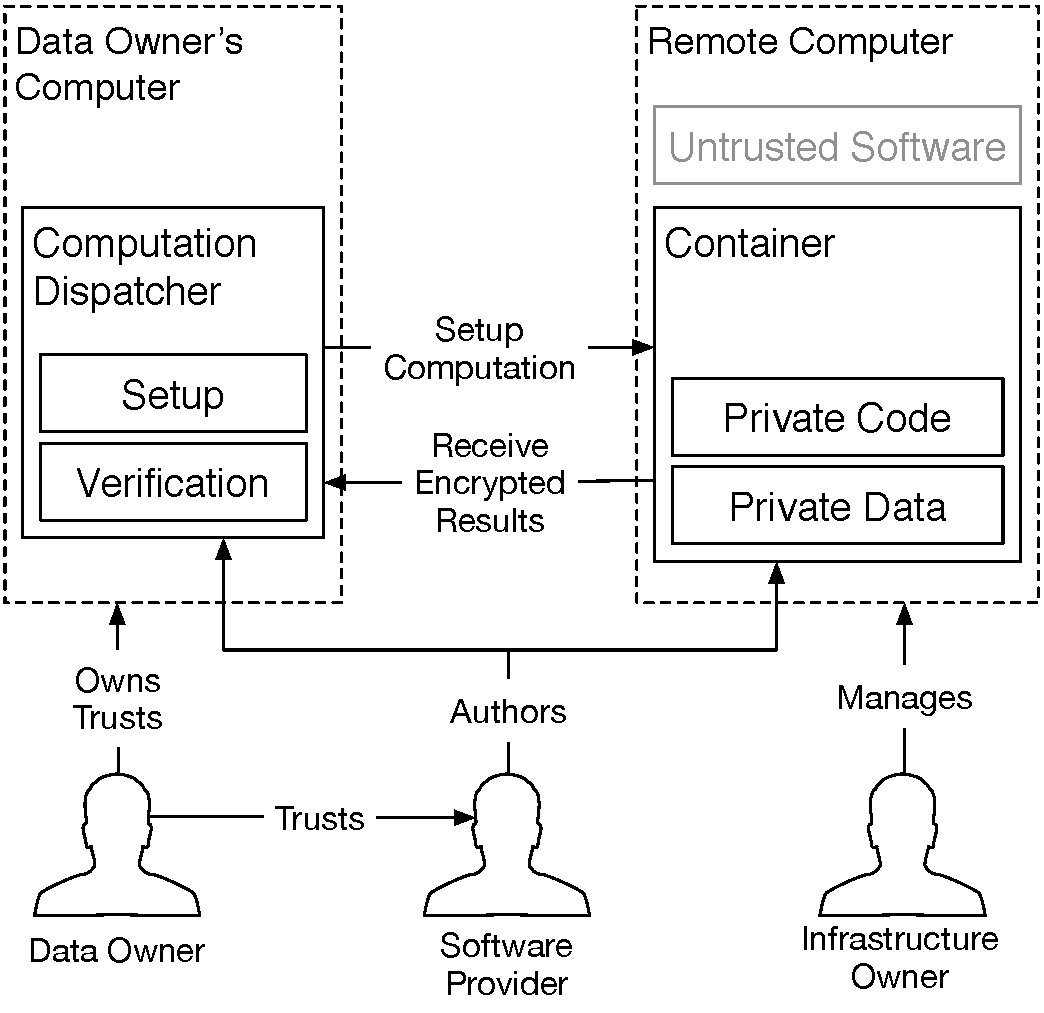
\includegraphics[width=75mm]{figures/remote_computation.pdf}}
  \caption{
    Secure remote computation. A user relies on a remote computer, owned by an
    untrusted party, to perform some computation on her data. The user has some
    assurance of the computation's integrity and privacy.
  }
  \label{fig:remote_computation}
\end{figure}

Intel's Software Guard Extensions (SGX) is the latest iteration in a long line
of trusted computing (Figure~\ref{fig:trusted_computing}) designs, which aim to
solve the secure remote computation problem by leveraging trusted hardware in
the remote computer. The trusted hardware establishes a secure container, and
the remote computation service user uploads the desired computation and data
into the secure container. The trusted hardware protects the data's privacy
and integrity while the computation is being performed on it.

\begin{figure}[hbt]
  \center{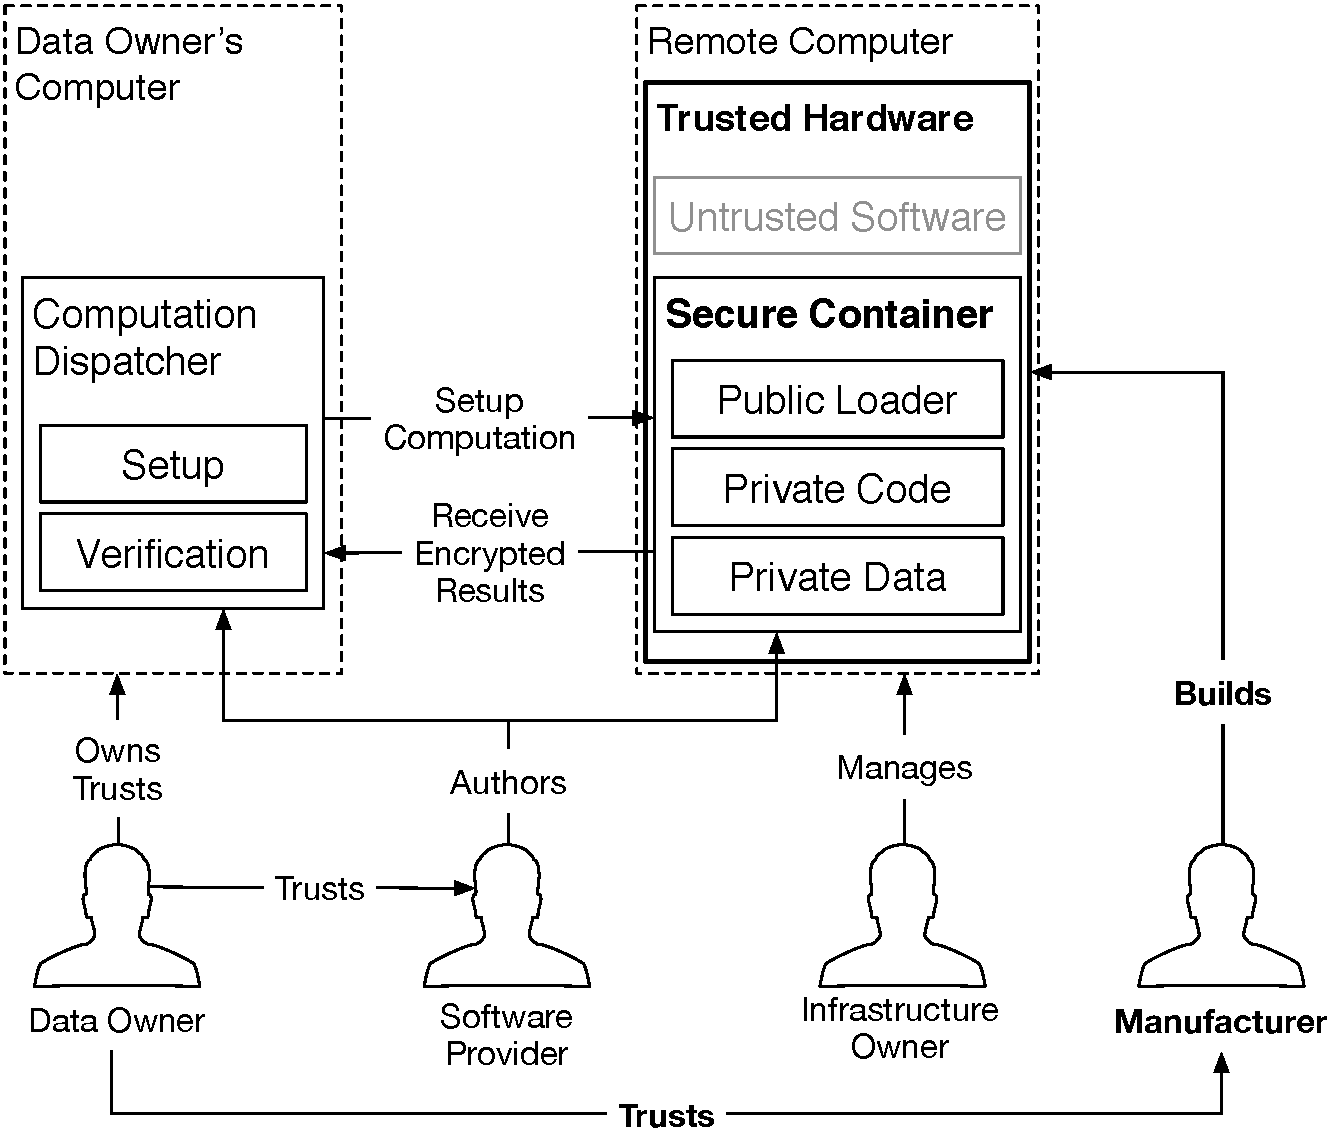
\includegraphics[width=85mm]{figures/trusted_computing.pdf}}
  \caption{
    Trusted computing. The user trusts the manufacturer of a piece of hardware
    in the remote computer, and entrusts her data to a secure container hosted
    by the secure hardware.
  }
  \label{fig:trusted_computing}
\end{figure}

SGX relies on \textit{software attestation}, like its predecessors, the
TPM~\cite{grawrock2003tpm} and TXT~\cite{grawrock2009txt}. Attestation
(Figure~\ref{fig:generic_attestation}) proves to a user that she is
communicating with a specific piece of software running in a secure container
hosted by the trusted hardware. The proof is a cryptographic signature that
certifies the hash of the secure container's contents. It follows that the
remote computer's owner can load any software in a secure container, but the
remote computation service user will refuse to load her data into a secure
container whose contents hash that does not match the expected value.

\begin{figure}[hbt]
  \center{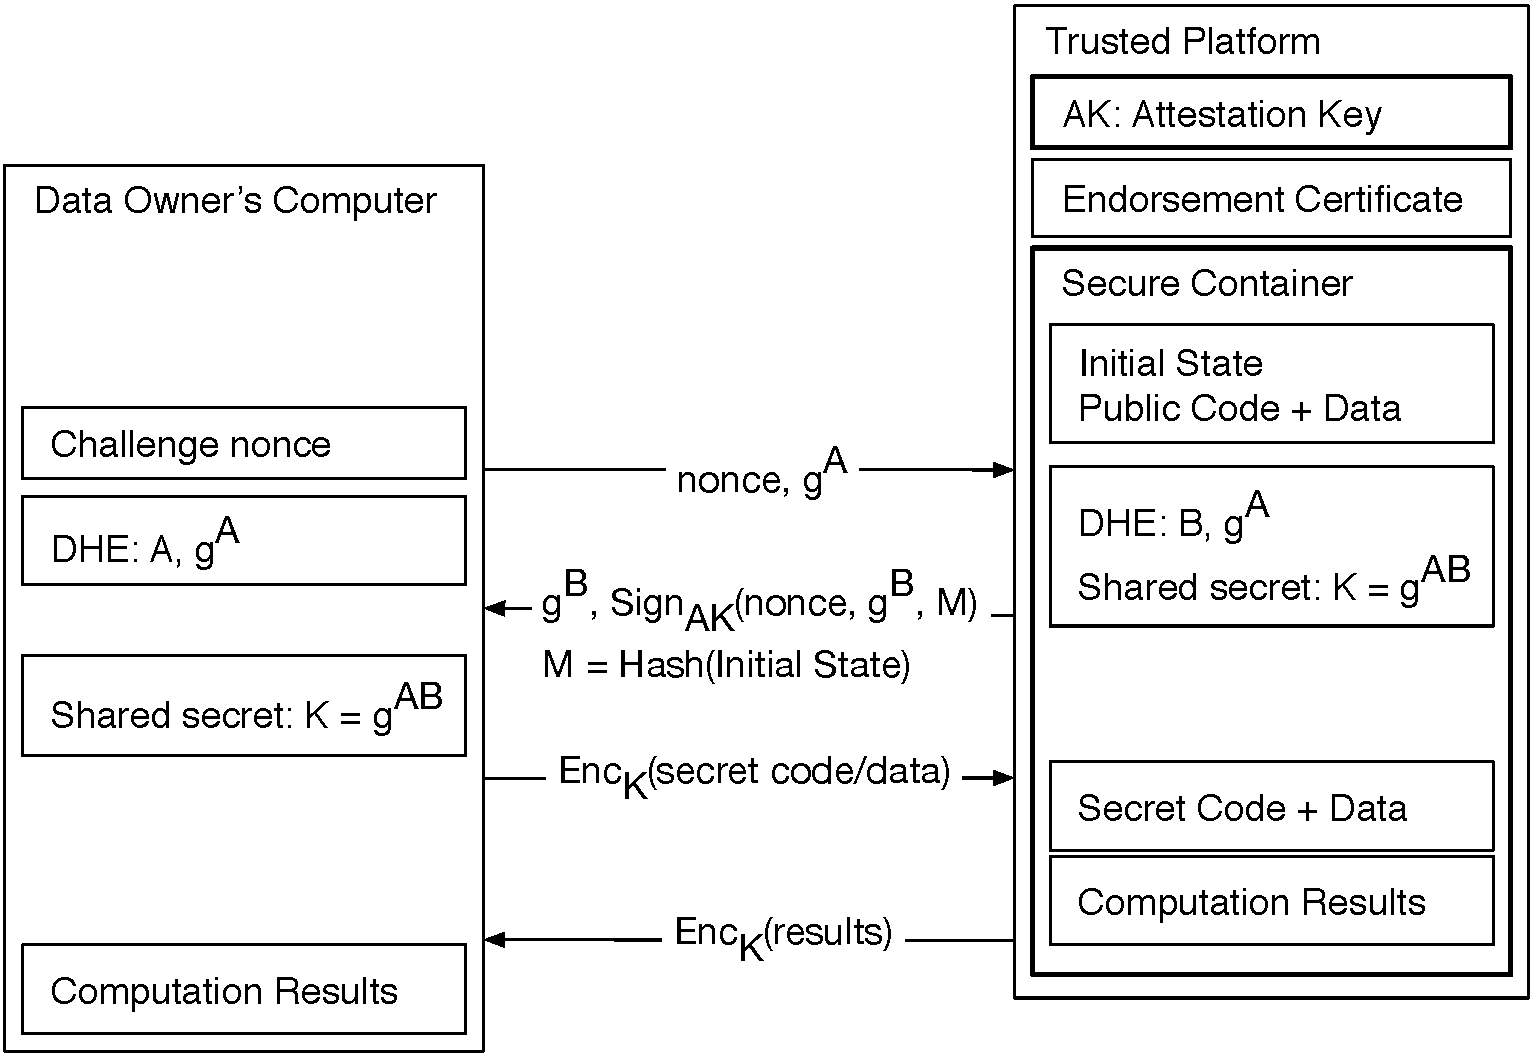
\includegraphics[width=85mm]{figures/generic_attestation.pdf}}
  \caption{
    Software attestation proves to a remote computer that it is communicating
    with a specific secure container hosted by a trusted platform. The proof is
    an attestation signature produced by the platform's secret attestation key.
    The signature covers the container's initial state, a challenge nonce
    produced by the remote computer, and a message produced by the container.
  }
  \label{fig:generic_attestation}
\end{figure}

The remote computation service user verifies the \textit{attestation key} used
to produce the signature against an \textit{endorsement certificate} created by
the trusted hardware's manufacturer. The certificate states that the
attestation key is only known to the trusted hardware, and only used for the
purpose of attestation.

SGX stands out from its predecessors by the amount of code covered by the
attestation, which is in the Trusted Computing Base (TCB) for the system using
hardware protection. The attestations produced by the original TPM design
covered all the software running on a computer, and TXT attestations covered
the code inside a VMX \cite{uhlig2005vmx} virtual machine. In SGX, an
\textit{enclave} (secure container) only contains the private data in a
computation, and the code that operates on it.

For example, a cloud service that performs image processing on confidential
medical images could be implemented by having users upload encrypted images.
The users would send the encryption keys to software running inside an enclave.
The enclave would contain the code for decrypting images, the image processing
algorithm, and the code for encrypting the results. The code that receives the
uploaded encrypted images and stores them would be left outside the enclave.

An SGX-enabled processor protects the integrity and privacy of the computation
inside an enclave by isolating the enclave's code and data from the outside
environment, including the operating system and hypervisor, and hardware
devices attached to the system bus. At the same time, the SGX model remains
compatible with the traditional software layering in the Intel architecture,
where the OS kernel and hypervisor manage the computer's resources.


\subsection{SGX Lightning Tour}
\label{sec:intro_sgx}

SGX sets aside a memory region, called the \textit{Processor Reserved Memory}
(PRM, \S~\ref{sec:prm}). The CPU protects the PRM from all non-enclave memory
accesses, including kernel, hypervisor and SMM (\S~\ref{sec:rings}) accesses,
and DMA accesses (\S~\ref{sec:motherboard}) from peripherals.

The PRM holds the \textit{Enclave Page Cache} (EPC, \S~\ref{sec:epc}), which
consists of 4KB pages that store enclave code and data. The system software,
which is untrusted, is in charge of assigning EPC pages to enclaves. The CPU
tracks each EPC page's state in the \textit{Enclave Page Cache Metadata} (EPCM,
\S~\ref{sec:epcm}), to ensure that each EPC page belongs to exactly one
enclave.

The initial code and data in an enclave is loaded by untrusted system software.
During the setup stage (\S~\ref{sec:lifecycle}), the system software asks the
CPU to copy data from unprotected memory (outside PRM) into EPC pages, and
assigns the pages to the enclave being setup (\S~\ref{sec:epcm}). This
means that the initial enclave state is known to the system software.

After all the enclave's pages are loaded into EPC, the system software asks the
CPU to mark the enclave as initialized, at which point application software can
run the code inside the enclave. After an enclave is initialized, the loading
method described above is disabled.

While an enclave is loaded, its contents is cryptographically hashed by the
CPU. When the enclave is initialized, the hash is finalized, and becomes the
enclave's \textit{measurement hash}.

A remote party can undergo an \textit{attestation} process to convince itself
that it is communicating with a specific enclave running in a secure
environment. The remote party generates a random challenge and sends it to the
enclave. After an intricate sequence of steps, the remote party receives an
\textit{attestation signature} that covers the challenge, the enclave's
measurement hash, and a message generated by the enclave. The attestation
signature is created by a secret CPU attestation key, which is covered by an
\textit{attestation certificate} rooted at Intel's manufacturer key.

Provided that the remote party trusts Intel's root key, attestation convinces
it that the message in the attestation was generated by a specific enclave
running in an SGX environment. If the message is a step in a Diffie-Hellman key
exchange, the remote party can be assured that the resulting symmetric key is
only shared between it and the attested enclave.

\section{Background}
\label{sec:background}

Arguing about the security of an application running on an mainstream computer
using the Intel architecture requires understanding the interactions between
all the parts of an x86 execution environment. This section provides an
overview of the features referenced by the rest of the paper. Unless specified
otherwise, the information in this section can be found in Intel's
\textit{Software Development Manual} \cite{intel2014sdm} (SDM).

Each of the sub-sections below explains how its information is relevant to
to SGX, but does not introduce any SGX concepts. Experienced readers can safely
skip this section and refer back if necessary.


\subsection{Software Privilege Levels}
\label{sec:rings}

In an Infrastructure-as-a-Service (IaaS) cloud environment, such as Amazon EC2,
commodity CPUs run software at four different privilege levels, illustrated in
Figure~\ref{fig:cpu_rings} and described below. The rest of the section
describes the privilege levels. We also point to successful exploits that
execute at each privilege level, motivating the SGX design decision to assume
that the host computer has malicious software running at all privilege levels.

\begin{figure}[hbtp]
  \center{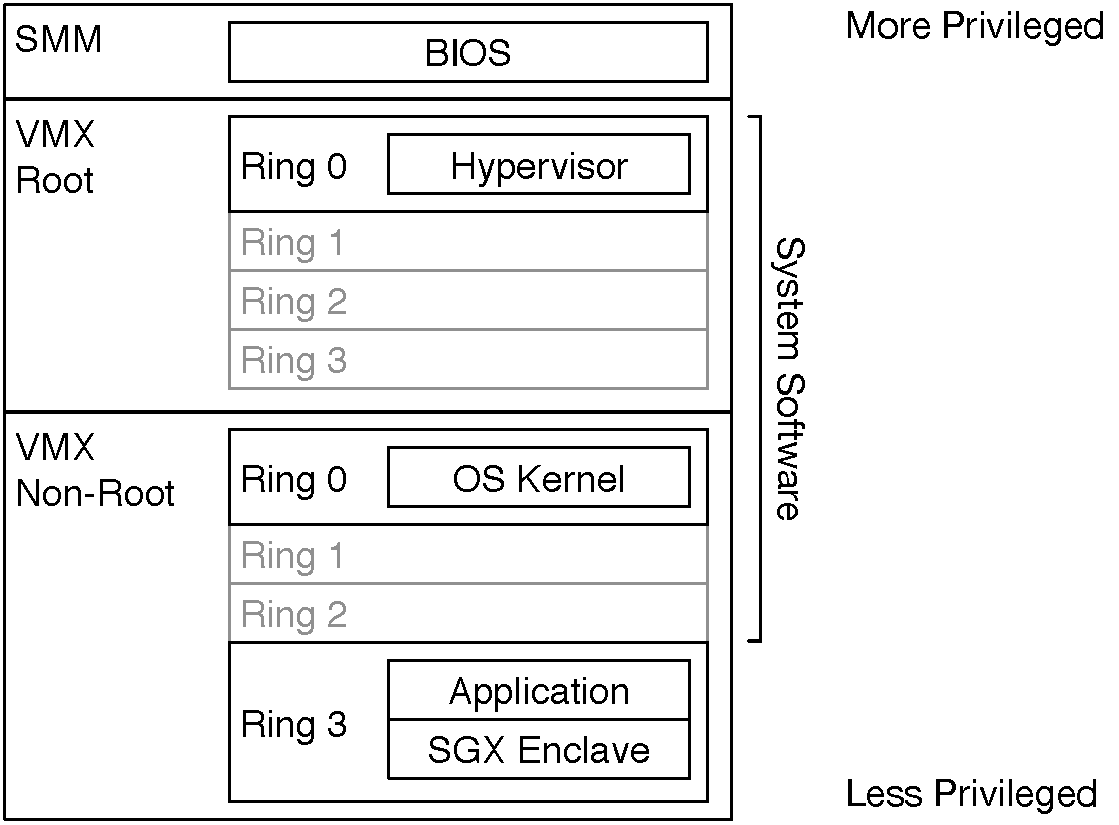
\includegraphics[width=50mm]{figures/cpu_rings.pdf}}
  \caption{
    The privilege levels in the x86 architecture, and the software that
    typically runs at each security level.
  }
  \label{fig:cpu_rings}
\end{figure}

\textit{System Management Mode} (SMM) is intended for use by the motherboard
manufacturers to implement features such as fan control and deep sleep, and/or
to emulate missing hardware. SMM mode is entered by asserting the SMI\# pin on
the CPU, which was initially designed exclusively for hardware use. However,
the southbridges on most motherboards provide a method for privileged
code\footnote{the hypervisor or operating system kernel} to get the SMI\# pin
asserted\footnote{Most southbridges assert \texttt{SMI\#} when a byte is
  written to port 0xb2 via the \textsc{out} opcode}.
This opens up the avenue for SMM-based software exploits.

The SMM code and data are stored in a contiguous subset of RAM called
\textit{System Management RAM} (SMRAM), which, in theory, is not readable or
writable when the processor isn't running in SMM. However, its protection
mechanisms were bypassed multiple times \cite{duflot2006smm}
\cite{rutkowska2008remap} \cite{wojtczuk2009smm}, and SMM-based rootkits have
been demonstrated \cite{wecherowski2009smm} \cite{embleton2010smm}.

IaaS cloud providers allow their customers to run their operating system of
choice in a virtualized environment. Hardware
virtualization\cite{uhlig2005vmx}, called \textit{Virtual Machine Extensions}
(VMX) by Intel, adds support for a \textit{hypervisor}, also called a
Virtual Machine Monitor (VMM) in the Intel documentation. The hypervisor runs
at a higher privilege level (VMX root mode) than the operating system, and is
responsible for allocating hardware resources across multiple operating systems
that share the same physical machine. The hypervisor uses the CPU's hardware
virtualization features to make each operating system believe it is running in
its own computer, called a \textit{virtual machine} (VM). Hypervisor code
generally runs at ring 0 in VMX root mode.

The popular Xen hypervisor uses VMX root mode for improved peformance and a
smaller codebase \cite{zhang2008xen}. \cite{mccune2010trustvisor} proposes
using a hypervisor together with Intel TXT's dynamic root of trust for
measurement (DRTM) to implement trusted execution.
\cite{vasudevan2010requirements} argues that a dynamic root of trust mechanism,
like Intel TXT, is necessary to ensure a hypervisor's integrity. Unfortunately,
the TXT design requires an implementation complex enough that security
vulnerabilities have been found \cite{wojtczuk2009txt2} \cite{wojtczuk2011txt}.
Furthermore, any SMM attack can be used to compromise TXT
\cite{wojtczuk2009txt}.

The systems research literature recommends breaking up an operating system into
a small \textit{kernel}, which runs at a high privilege level, known as the
\textit{kernel mode} or \textit{system mode} and, in the Intel architecture, as
\textit{ring 0}. The kernel allocates the computer's resources to the other
system components, such as device drivers and services, which run at lower
privilege levels. However, for performance reasons\footnote{Switching between
rings is much slower than a normal procedure call.}, mainstream operating
systems have large amounts of code running at ring 0. Their \textit{monolithic
kernels} include device drivers, filesystem code, networking stacks, and video
rendering functionality.

The monolithic kernel design leads to many opportunities for security
vulnerabilities in kernel code. For example the Linux kernel has had a
significant number of vulnerabilities patched every year, for the past 10 years
\cite{cvedetails2014linux} \cite{chen2011linux}. Also, a successful attack on
SMM or the hypervisor trivially translates into a compromised kernel.

Application code, such as a Web server or a game client, runs at the lowest
privilege level, referred to as \textit{user mode} (\textit{ring 3} in the
Intel architecture). In IaaS cloud environments, the virtual machine images
provided by customers run in VMX non-root mode, so the kernel runs in VMX
non-root ring 0, and the application code runs in VMX non-root ring 3.


\subsection{Address Translation}
\label{sec:paging}

Modern OS kernels rely on address translation to multiplex a computer's RAM
among multiple processes. In turn, hypervisors use address translation to
multiplex the RAM among that operating systems that run concurrently. The
software running inside a SGX enclave is subject to address translation, and
the implementation of SGX relies heavily on the translation implementation in
Intel processors. This section summarizes the Intel-specific software-visible
details needed to understand SGX, while \S~\ref{sec:tlbs} covers some
architectural specifics. \cite{jacob1998virtual} describes the generic concepts
and applications of address translation.

The Intel architecture specifies many address translation modes, used to run
legacy software dating back to 1990 natively. Most modes are not necessary for
understanding SGX, so we only cover the translation modes used in modern 64-bit
operating systems and 64-bit cloud environments.

64-bit desktop operating systems use the addressing mode called IA-32e by
Intel's documentation, which translates 48-bit \textit{virtual addresses} into
\textit{physical addresses} of at most 52 bits\footnote{The size of a physical
  address is CPU-dependent, and is 40 bits for recent desktop CPUs and 44 bits
for recent high-end server CPUs.}.  Figure~\ref{fig:os_paging} illustrates the
address translation process. The bottom 12 bits of a virtual address are not
changed by the translation. The top 36 bits are grouped into four 9-bit indexes
used to navigate a data structure called \textit{the page tables}. Despite its
name, the data structure closely resembles a perfectly balanced 512-ary search
tree where nodes have fixed keys.  Each node is an array of 512 8-byte entries
that contain the physical addresses of the next-level children as well as some
flags. The address of the root node is stored in the CR3 register. The arrays
in the last-level nodes contain the physical addresses that are the result of
the address translation.

\begin{figure}[hbtp]
  \center{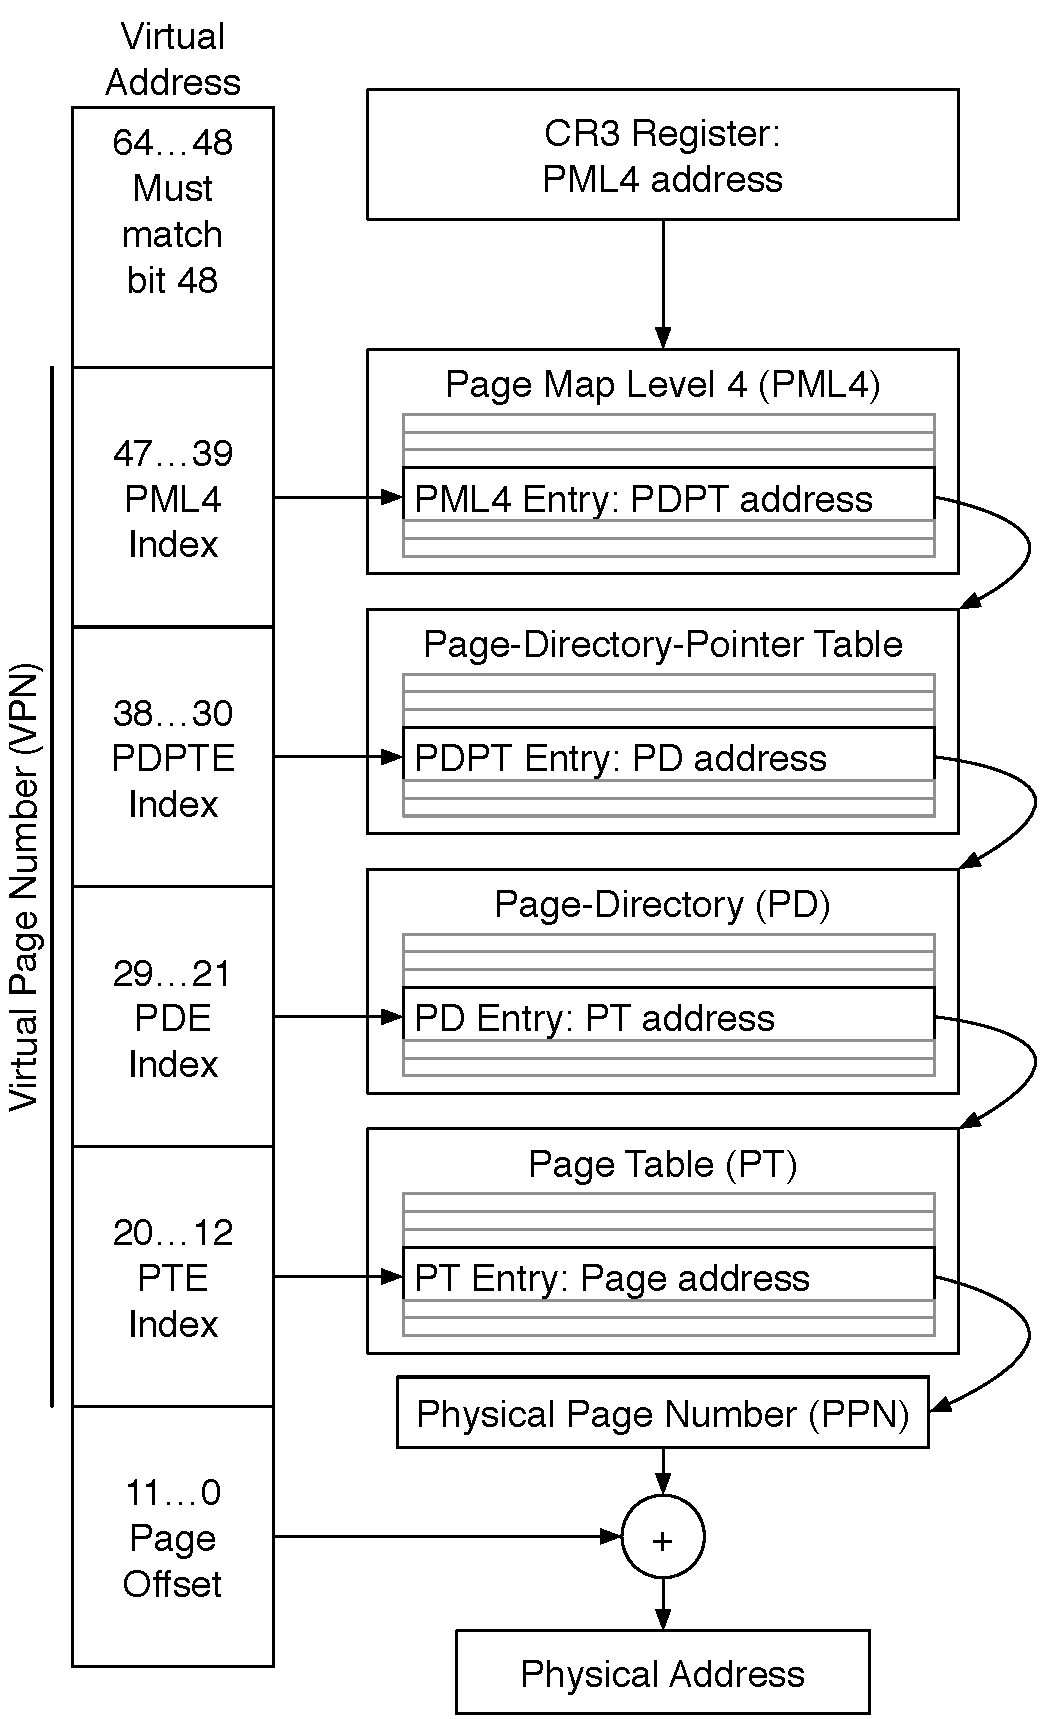
\includegraphics[width=85mm]{figures/os_paging.pdf}}
  \caption{
    IA-32e address translation takes in a 48-bit virtual address and outputs
    a 52-bit physical address.
  }
  \label{fig:os_paging}
\end{figure}

Hypervisors have access to another layer of address translation, named
\textit{extended page tables} (EPT), to multiplex the physical memory across
operating systems. When EPT are enabled, the process above is used to translate
from a virtual address into a \textit{guest-physical address}, effectively
giving each OS kernel the illusion that it controls the entire machine's RAM.
The translation from guest-physical addresses to actual physical addresses uses
the same process as above, except the physical address of the root node is
stored in the extended page table pointer (EPTP) field in the VM's control
structure (VMCS). Figure~\ref{fig:vmx_paging} illustrates the address
translation process in the presence of hardware virtualization.

\begin{figure}[hbtp]
  \center{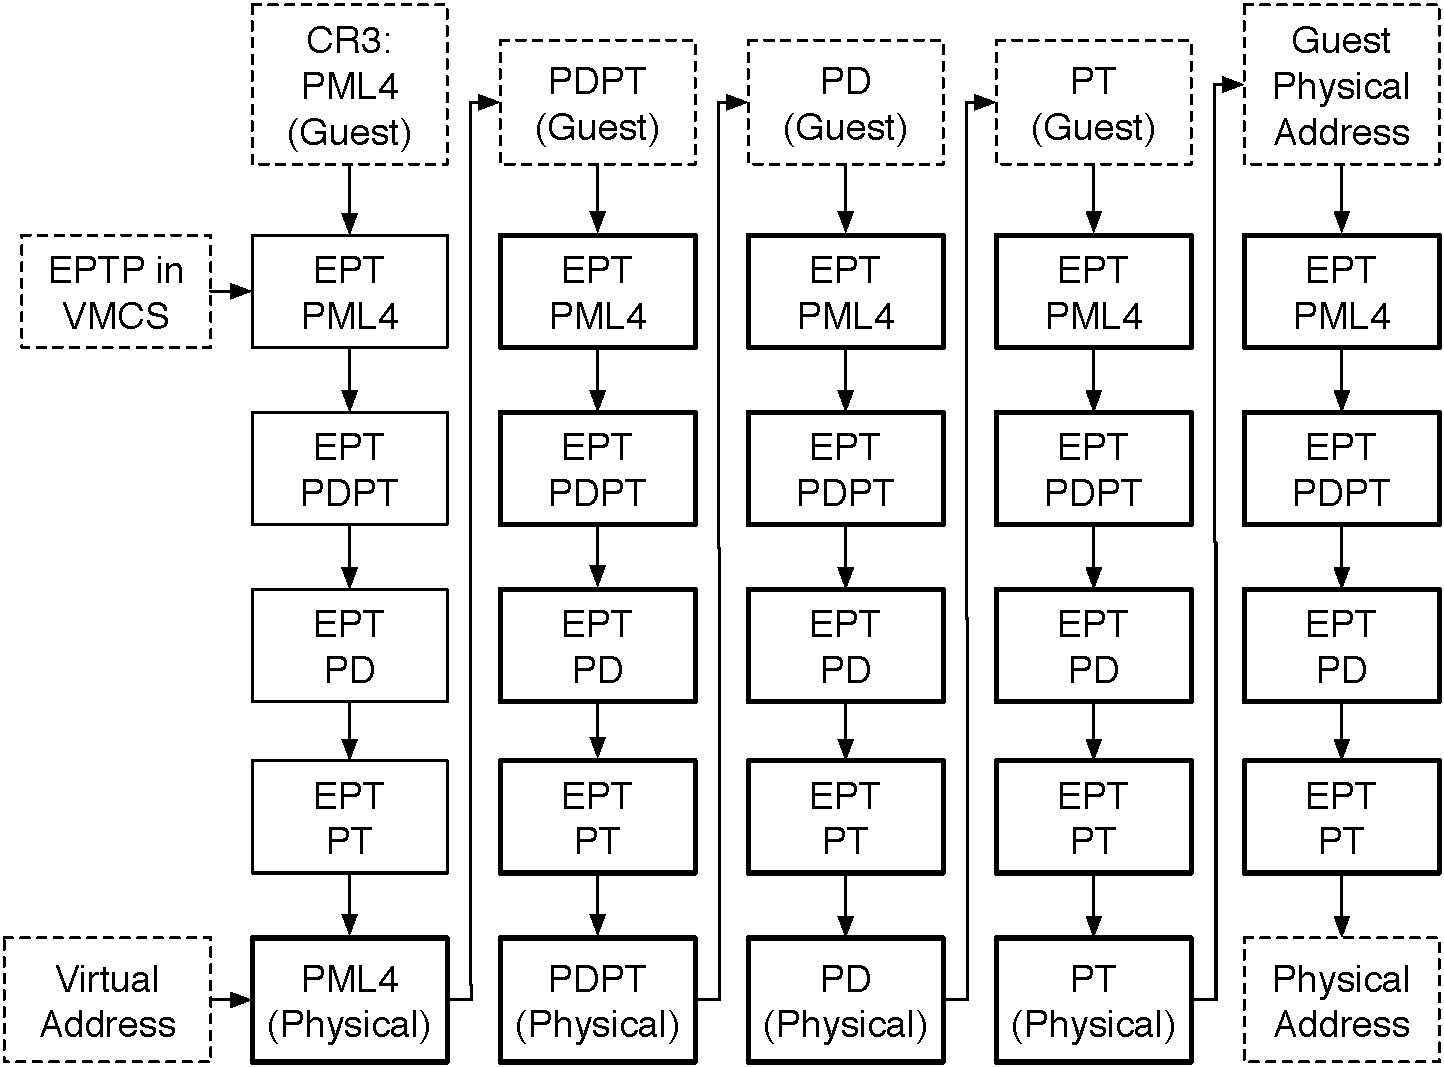
\includegraphics[width=85mm]{figures/vmx_paging.pdf}}
  \caption{
    Address translation when hardware virtualization is enabled. The
    kernel-managed page tables contain guest-physical addresses, so each level
    in the kernel's page table requires a full walk of the hypervisor's
    extended page table (EPT).  A translation requires up to 20 memory accesses
    (the bold boxes), assuming the physical address of the kernel's PML4 is
    cached.
  }
  \label{fig:vmx_paging}
\end{figure}

Each entry in the page tables has some boolean flags, in addition to the
pointer to the next level. The following flags are particularly interesting for
our goals. The \textit{present} (P) flag is set to 0 to indicate pages that
have been evicted from RAM to a cheaper and slower storage medium. When address
translation encounters a page table entry where P is 0, the CPU generates a
page fault (\#PF), and the OS kernel is responsible for loading the page back
into RAM and resuming execution. If an EPT entry has the P flag set to 0, the
CPU performs a VM exit, and the hypervisor has an opportunity to bring the page
into RAM. The \textit{accessed} (A) flag is set to 1 by the CPU whenever the
address translation machinery reads a page table entry, and the \textit{dirty}
(D) flag is set to 1 by the CPU when an entry is accessed by a memory write
operation. The A and D flags give the hypervisor and kernel insight into
application memory access patterns, providing the input for the algorithms that
select which pages get to be evicted from RAM.

Page table entries have flags that provide access control, in addition to the
flags supporting page swapping. The interesting flags are the \textit{writable}
(W) flag, which can be set to 0 to prohibit\footnote{Writes to non-writable
pages result in general protection faults (\#GP).} memory writes to a page, and
the \textit{disable execution} (XD) flag, which can be set to 1 to prevent
instruction fetches from a page.


\subsection{Context Switching}
\label{sec:registers}

Application software targeting the 64-bit Intel architecture uses a variety of
registers to interact with the CPU features. The values in these registers
make up an application's state, or context. Kernels multiplex a CPU among
multiple software threads by \textit{context switching}, namely saving a
thread's context, and replacing it with another thread's previously saved
context. This section covers the context switching features used by SGX when a
logical processor starts or stops executing code that belongs to an enclave.

\begin{figure}[hbt]
  \center{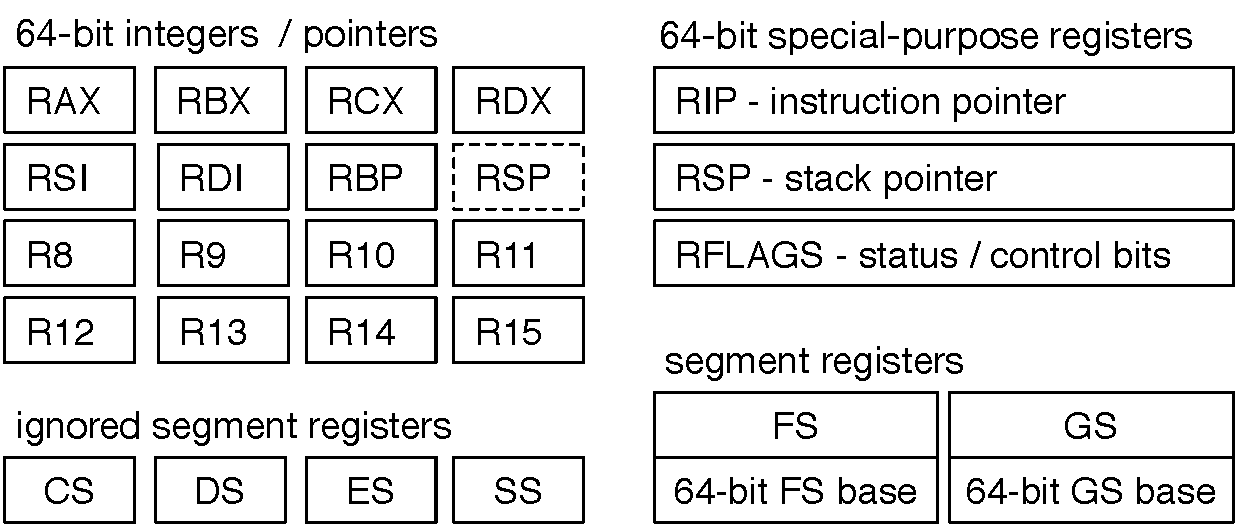
\includegraphics[width=85mm]{figures/cpu_registers.pdf}}
  \caption{
    CPU registers in the 64-bit Intel architecture. RSP can be used as a
    general-purpose register (GPR), e.g., in pointer arithmetic, but it always
    points to the top of the program's stack.
  }
  \label{fig:cpu_registers}
\end{figure}

Integers and memory addresses are stored in 16 \textit{general-purpose
registers} (GPRs). RAX, RBX, RCX, RDX, RSI, RDI, RSP, and RBP are extended
versions of the GPRs available to 32-bit programs, and R9-R16 are new
registers. RSP is reserved for pointing to the top of the \textit{stack}, which
is used to save state during procedure calls.

In 64-bit mode, the values of most segment registers (CS, DS, ES, SS) are
ignored. The FS and GS segment registers generally point to the current
thread's \textit{thread-local storage}, so they are still partially supported
in 64-bit mode. The base addresses loaded in FS and GS are used when computing
linear addresses, whereas the limits are ignored.

All applications also use the RIP register, which contains the address of the
currently executing instruction, and the RFLAGS register, whose bits (e.g.,
the carry flag - CF) are individually used to store comparison results and
control various instructions.

Software might use other registers to interact with specific features, some of
which are shown in Table~\ref{fig:xsave_state}.

\begin{table}[hbt]
  \center{\begin{tabularx}{\columnwidth}{| l | X | l |}
  \hline
  \textbf{Feature} & \textbf{Registers} & \textbf{Feature bit}\\
  \hline
  FPU & FP0 - FP7, FSW, FTW & 0 \\
  \hline
  SSE & MM0 - MM7, XMM0 - XMM15, XMCSR & 1 \\
  \hline
  AVX & YMM0 - YMM15 & 2 \\
  \hline
  \end{tabularx}}
  \caption{Sample feature-specific Intel architecture registers.}
  \label{fig:xsave_state}
\end{table}

The Intel architecture provides a future-proof method for an OS kernel to save
the values of feature-specific registers used by an application. The XSAVE
instruction takes in a bitmap of features, and writes the registers used by
the features whose bits are set to 1 in a memory area that can be used by the
XRESTORE instruction to load the saved values back into feature-specific
registers.

Application software declares the features that it plans to use to the kernel,
so the kernel knows what XSAVE bitmap to use when context-switching. When
receiving the system call, the kernel sets the XCR0 register to the feature
bitmap declared by the application. The CPU generates a fault if application
software attempts to use features that are not enabled by XCR0, so applications
cannot modify feature-specific registers that the kernel wouldn't take into
account when context-switching. The kernel can use the CPUID instruction to
learn the size of the XSAVE memory area for a given feature bitmap, and compute
how much memory it needs to allocate for the context of each of the
application's threads.


\subsection{A Computer Map}

This section maps out a computer using the Intel architecture at three zoom
levels: the motherboard, the CPU, and the execution core, focusing on the
concepts needed to understand SGX and analyze its security properties. Most
details in here are documented in Intel's
\textit{Optimization Reference Manual} \cite{intel2014optimization}.

\subsubsection{The Motherboard}
\label{sec:motherboard}

A computer's components are connected by a printed circuit board called a
\textit{motherboard}, which consists of \textit{sockets} connected by
\textit{buses}. Sockets connect chip-carrying \textit{packages}, to the board.
The Intel documentation uses the term ``package'' to specifically refer to a
CPU.

The buses most relevant to SGX (see Figure~\ref{fig:motherboard} are the
\textit{Quick-Path Interconnect} (QPI) \cite{intel2009qpi}, a network of
point-to-point links that connect processors, the \textit{double data rate}
(DDR) bus that connects a CPU to DRAM, and the \textit{Peripheral Component
Interconnect Express} (PCIe) bus that connects a CPU to peripherals such as a
\textit{Network Interface Card} (NIC).

\begin{figure}[hbt]
  \center{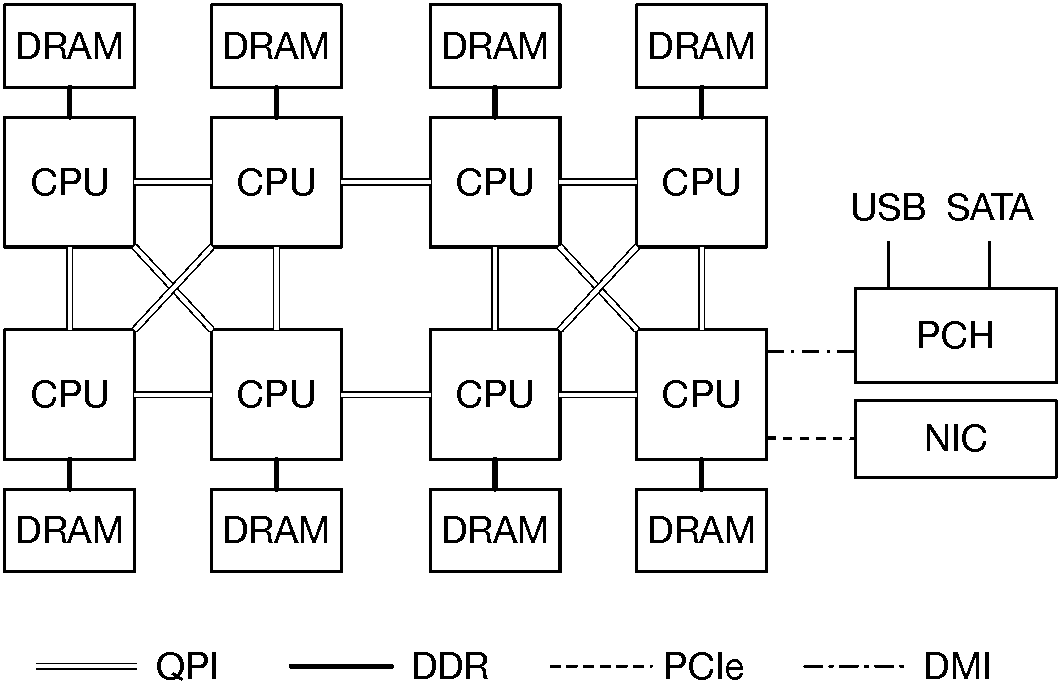
\includegraphics[width=45mm]{figures/motherboard.pdf}}
  \caption{
    The motherboard structures that are most relevant to SGX.
  }
  \label{fig:motherboard}
\end{figure}

The SGX trusted computing base includes the processor package, and excludes the
other hardware in the computer. This implies that, SGX must be able to fend off
attacks from rogue devices, such as the PCIe NIC used to compromise Intel TXT
\cite{wojtczuk2011txt}, as well as passive or active bus-tapping attacks, such
as the memory bus tap used to hack the Xbox \cite{huang2003xbox} and the
memory glitching attack that subverted the PlayStation 3 hypervisor
\cite{hotz2010ps3}.

\subsubsection{The Processor}
\label{sec:cpu_die}

An Intel processor's die, illustrated in Figure~\ref{fig:cpu_die}, is divided
into two broad areas: the \textit{core area} implements the functionality that
comes to mind when thinking of a CPU, while the \textit{uncore} provides
functions that were typically hosted on separate chips, but were integrated to
save power and improve latency.

\begin{figure}[hbt]
  \center{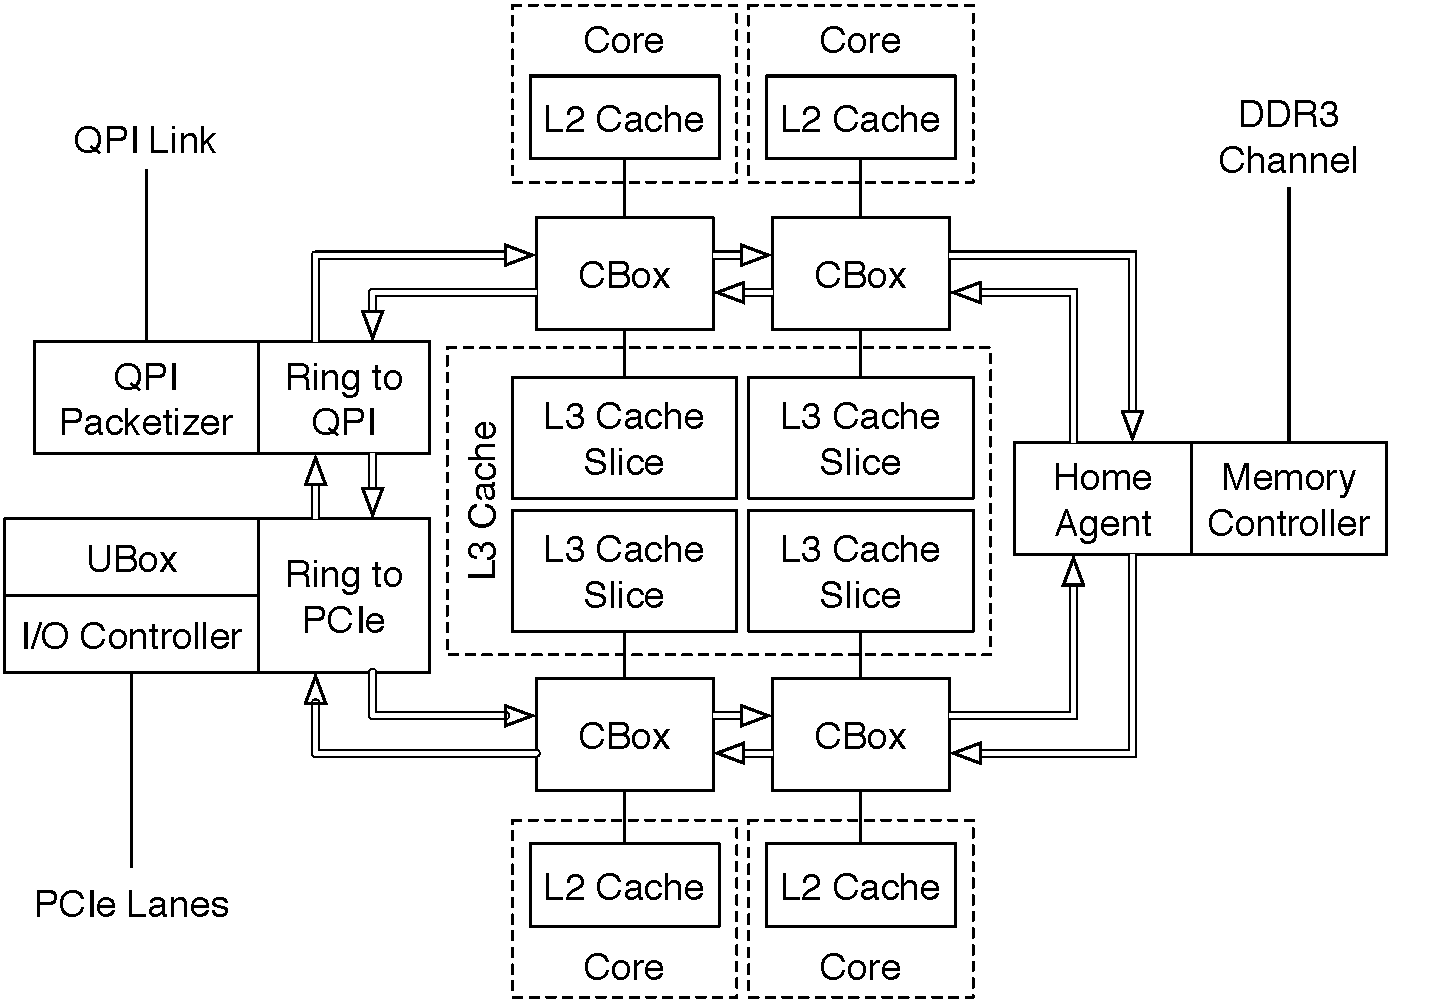
\includegraphics[width=85mm]{figures/cpu_die.pdf}}
  \caption{
    The major components in a modern CPU die. \S~\ref{sec:cpu_die} gives
    an uncore overview. \S~\ref{sec:cpu_core} describes execution cores.
    \S~\ref{sec:cpu_uncore} takes a deeper look at the uncore.
  }
  \label{fig:cpu_die}
\end{figure}

At a conceptual level, the uncore of modern processors includes a memory
controller that interfaces with the DDR bus, an I/O controller that can
arbitrate the PCIe bus, and a growing number of integrated controllers for
peripherals, such as a NIC and a GPU.

The SGX design relies on the fact that the processor die includes the memory
and I/O controller, and thus can prevent any device from accessing protected
memory areas via \textit{Direct Memory Access} (DMA) transfers.
\S~\ref{sec:cpu_uncore} takes a deeper look at the uncore organization and at
the mechanism used by the SGX implementation to protect sensitive memory.

\subsubsection{The Core}
\label{sec:cpu_core}

Virtually all modern Intel processors have core areas consisting of multiple
copies of the execution core circuitry, each of which is called a
\textit{core}.  At the time of this writing, desktop-class Intel CPUs have 4
cores, and server-class CPUs have as many as 18 cores.

Most Intel CPUs feature \textit{hyper-threading}, which means that a core
(shown in Figure~\ref{fig:cpu_core}) has two copies of the register files
backing the execution context described in \S~\ref{sec:registers}, and can
execute two separate streams of instructions simultaneously. Hyper-threading
increases the utilization of the shared fetch, decode and execution units, in
the presence of memory stalls.

\begin{figure}[hbt]
  \center{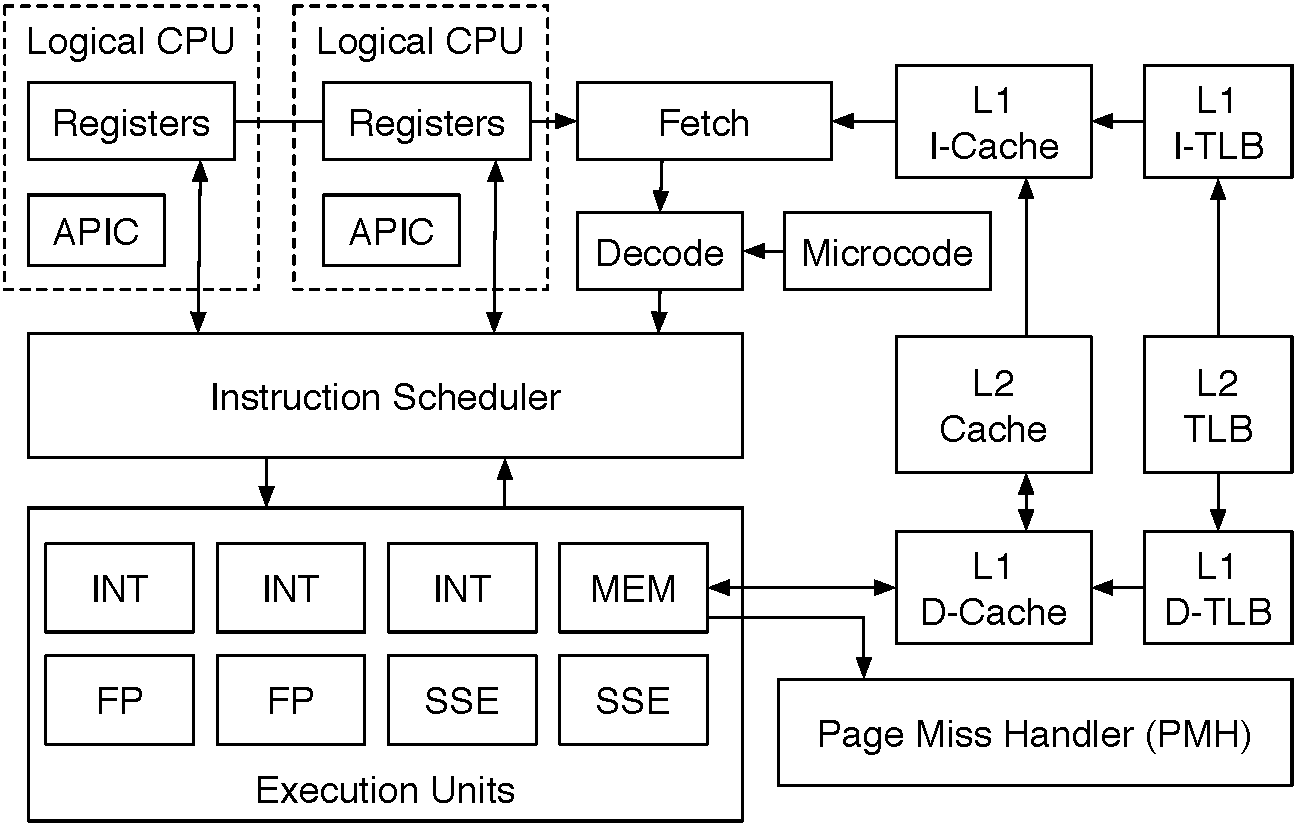
\includegraphics[width=85mm]{figures/cpu_core.pdf}}
  \caption{
    CPU core with two logical processors. Each logical processor has its own
    execution context and local APIC, and they share all the other core
    resources.
  }
  \label{fig:cpu_core}
\end{figure}

A hyper-threaded core is exposed to system software as two \textit{logical
processors}, also named \textit{hardware threads} in the Intel documentation.
The logical processor abstraction allows the code used to distribute work
across processors in a multi-processor system to function without any change on
multi-core hyper-threaded processors.

The high level of resource sharing introduced by hyper-threading introduces a
security vulnerability. Software running on one logical processor can use the
high-performance counter \cite{petters1999making} to get information about the
instructions and memory access patterns of another piece of software that is
executed on the other logical processor in the same core.


\subsection{CPU Microcode}
\label{sec:microcode}

Intel's SGX patents disclose that all the SGX features, except for DRAM
encryption, were implemented as microcode extensions. This section explains the
microcode feature in Intel CPUs. The limitations of microcode can explain
seemingly arbitrary decisions in the SGX design, and a thorough understanding
is crucial to evaluating the feasibility of SGX modification proposals.

The x86 architecture defines a \textit{complex instruction set} (CISC).
However, virtually all modern CPUs are architected following \textit{reduced
instruction set} (RISC) principles. This is accomplished by having the
instruction decode stage (see Figure~\ref{fig:cpu_core}) break down each x86
instruction into \textit{micro-ops} for every instruction. The other CPU stages
work exclusively with micro-ops.

The majority of x86 instructions are handled by the hardware decoding path,
which can emit at most 4 micro-ops per instruction. Complex instructions use a
slower decoding path that reads micro-ops from a \textit{microcode store ROM}
(MSROM).

Modern Intel processors implement a microcode update facility. The SDM
describes microcode updates from the perspective of an OS kernel and
hypervisor. Each core can be updated independently, and the updates must be
re-applied on each boot cycle. A core can be updated multiple times, but each
update must have a bigger version than the core's current version.

The update facility increases the attractiveness of developing architectural
features as microcode extensions. The SGX enclave measurements produced by the
processor include the microcode version, hinting that the SGX designers
anticipated the need to use microcode updates.

\cite{hawkes2012microcode} used fault injection and timing analysis to conclude
that each recent Intel microcode update is signed with a 2048-bit RSA key and
a (possibly non-standard) 256-bit hash algorithm. This implies that Intel
already has a microcode implementation of RSA-2048 signature checking, which
may explain why SGX uses RSA signatures in its enclave structures.

\cite{chen2014microcode} sets out to analyze the structure of microcode used in
all x86 processors, but is unable to obtain any details about Intel's
microcode. Fortunately, even though the microcode structure is undocumented,
the 4 micro-ops limitation can be used to guess intelligently whether an
architectural feature is implemented in microcode. For example, the context
switch in \S~\ref{sec:registers} is most likely done in microcode, whereas
simple arithmetic and memory access is handled directly by hardware.


\subsection{Memory Caching}
\label{sec:caching}

Caches are small, fast memories that store recently accessed code and data.
Thanks to the high locality in the memory access patterns of most applications,
good caches have very high hit rates (90\%-99\%), and do a great job of hiding
the (comparatively) high latency of DRAM. At the same time, the large time
differences between cached and un-cached memory accesses can be used to learn
about an application's memory access patterns, via
\textit{cache timing attacks} \cite{banescu2011cache}. The patterns, in turn,
can reveal private information, such as whether certain bits in an encryption
key are set or not.

This section describes the caching concepts needed to understand our claim that
cache timing attacks can be used to obtain fine-grained memory access patterns
for the software running inside an SGX enclave. \cite{smith1982cache},
\cite{patterson2013architecture} and \cite{hennessy2012architecture} all
provide good backgrounds on low-level cache implementation concepts.

Desktop-class Intel CPUs have three levels of cache memory. Each core has its
own L1 and L2, and all cores share an L3 cache. This means that a cache timing
attack that aims at the L2 cache would have to rely on the hypervisor or kernel
to schedule a hardware thread on a logical processor in the same core as the
target software, whereas an attack on the L3 cache can be performed using any
logical processor on the same CPU.

The \textit{cache line} is the atomic unit of data transfer between the caches
and the main memory. The cache line size is always a power of two. Assuming
$n$-bit memory addresses and a cache line size of $2^{l}$ bytes, the lowest
$l$ bits of a memory address are an offset into a cache line, and the highest
$n - l$ bits determine the cache line that is used to store the data at the
memory location. All recent processors have 64-byte cache lines.

The L1 and L2 caches in recent processors are multi-way set-associative with
direct set indexing, as shown in Figure~\ref{fig:cpu_cache}. A $W$-way
set-associative cache has its memory divided into \textit{sets}, where each set
has $W$ lines. A memory location can be cached in any of the $w$ lines in a
specific set that is determined by the highest $n - l$ bits of the location's
memory address. Direct set indexing means that the $S$ sets in a cache are
indexed from $0$ to $S - 1$, and a memory location is cached in the set with
index $address_{n - 1 \ldots n - l} \bmod S$. In the common case where the
number of sets in a cache is a power of two, so $S = 2^{s}$, the lowest $l$
bits in an address make up the cache line offset, the next $s$ bits are the set
index. The highest $n - s - l$ bits in an address are not used when selecting
where a memory location will be cached. Figure~\ref{fig:cpu_cache} shows the
cache structure and lookup process.

\begin{figure}[hbt]
  \center{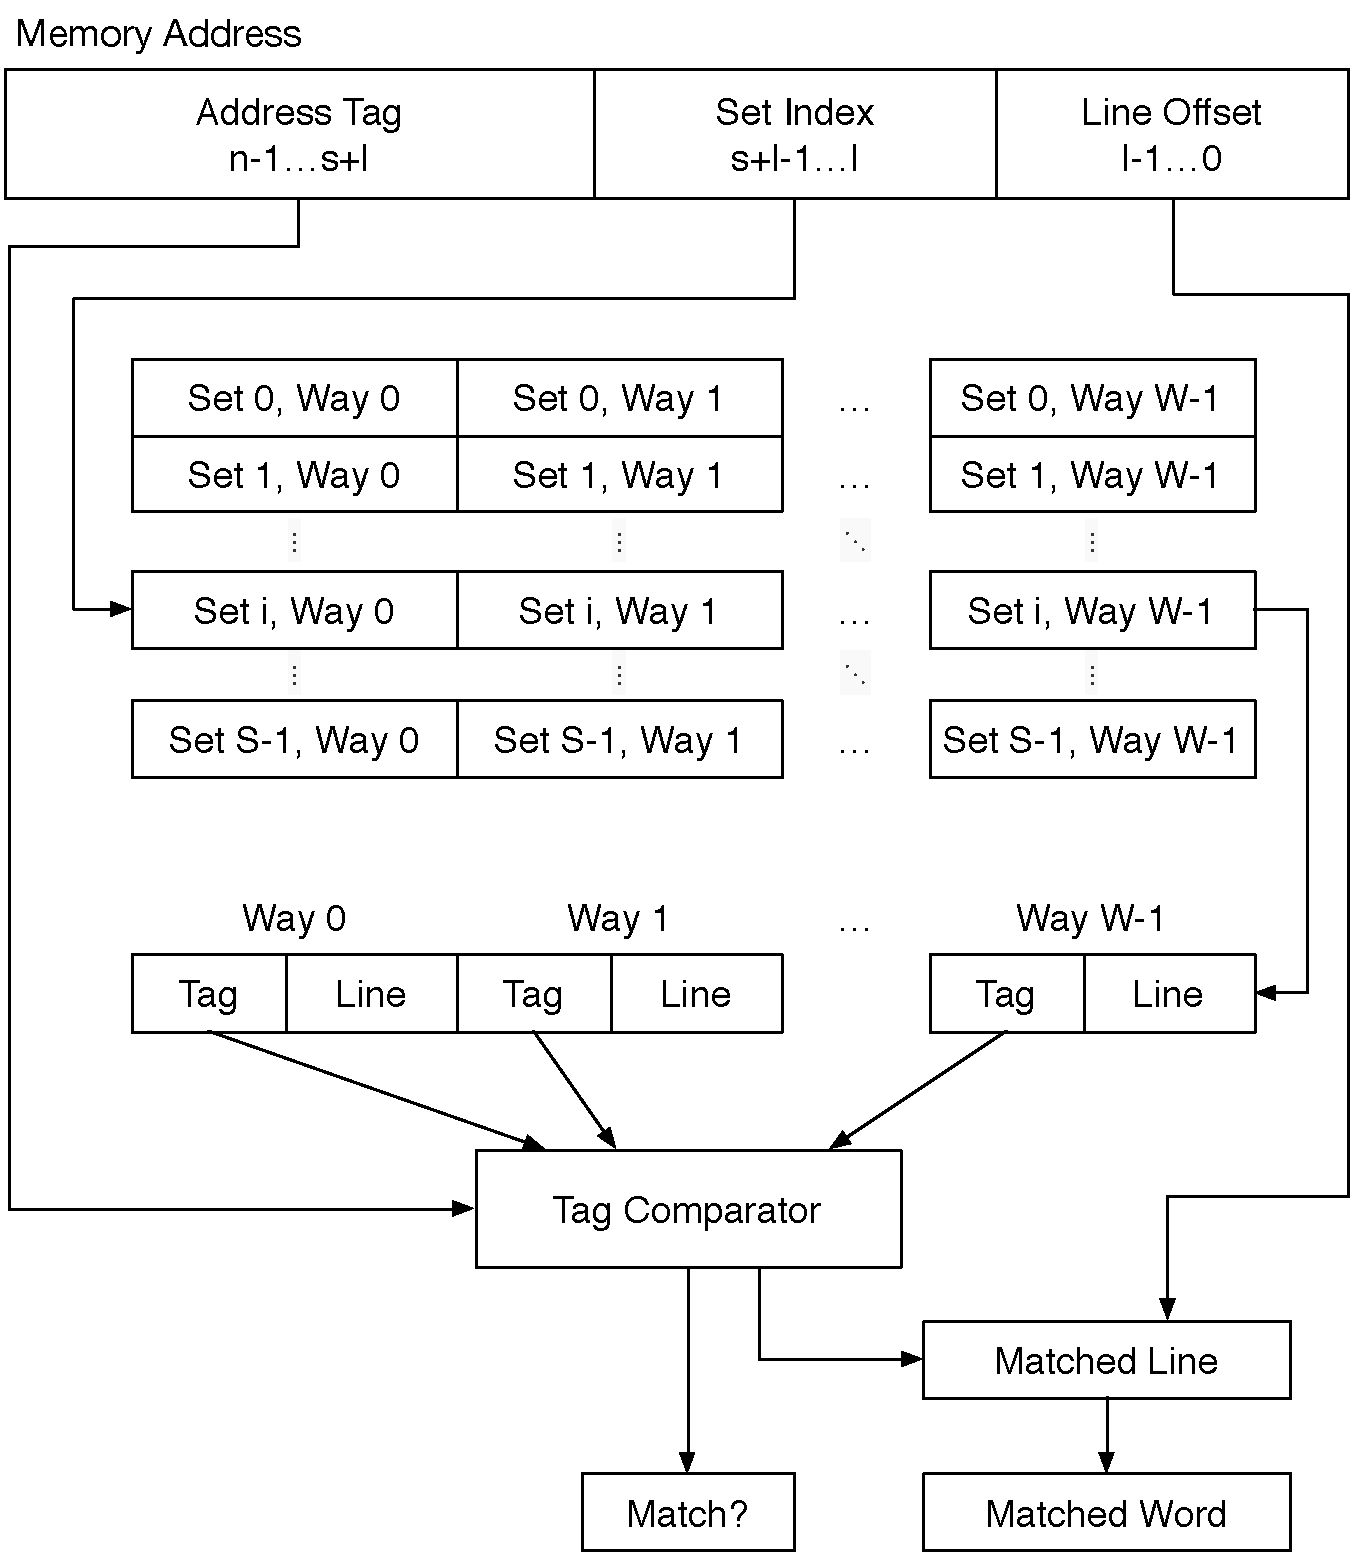
\includegraphics[width=85mm]{figures/cpu_cache.pdf}}
  \caption{
    Cache organization and lookup, for a $W$-way set-associative cache with
    $2^{l}$-byte lines and $S = 2^{s}$ sets. The cache works with $n$-bit
    memory addresses. The lowest $l$ address bits point to a specific byte in a
    cache line, the next $s$ bytes index the set, and the highest $n - s - l$
    bits are used to decide if the desired address is in one of the $W$ lines
    in the indexed set.
  }
  \label{fig:cpu_cache}
\end{figure}

The SDM does not describe the L3 indexing scheme, but we develop some
understanding of it in \S~\ref{sec:cpu_uncore}.


\subsection{Caching and Address Translation}
\label{sec:tlbs}

Address translation (described in \S~\ref{sec:paging}) requires up to 4 memory
accesses for a 64-bit bare-metal kernel, and up to 16 memory accesses when a
hypervisor is present. To achieve high clock speeds, the CPU caches address
translations in \textit{translation look-aside buffers} (TLBs).

The set index in an L1 cache only uses the address bits that are not impacted
by address translation, so that set lookup and TLB lookup can be done in
parallel. Given a page size $P = 2^{p}$ bytes, the requirement above is
equivalent to $l + s \le p$. In the x86 architecture $p = 12$, and all recent
processors have 64-byte cache lines ($l = 6$) and 64 sets ($s = 6$), as shown
in Figure~\ref{fig:caching_and_paging}.

\begin{figure}[hbt]
  \center{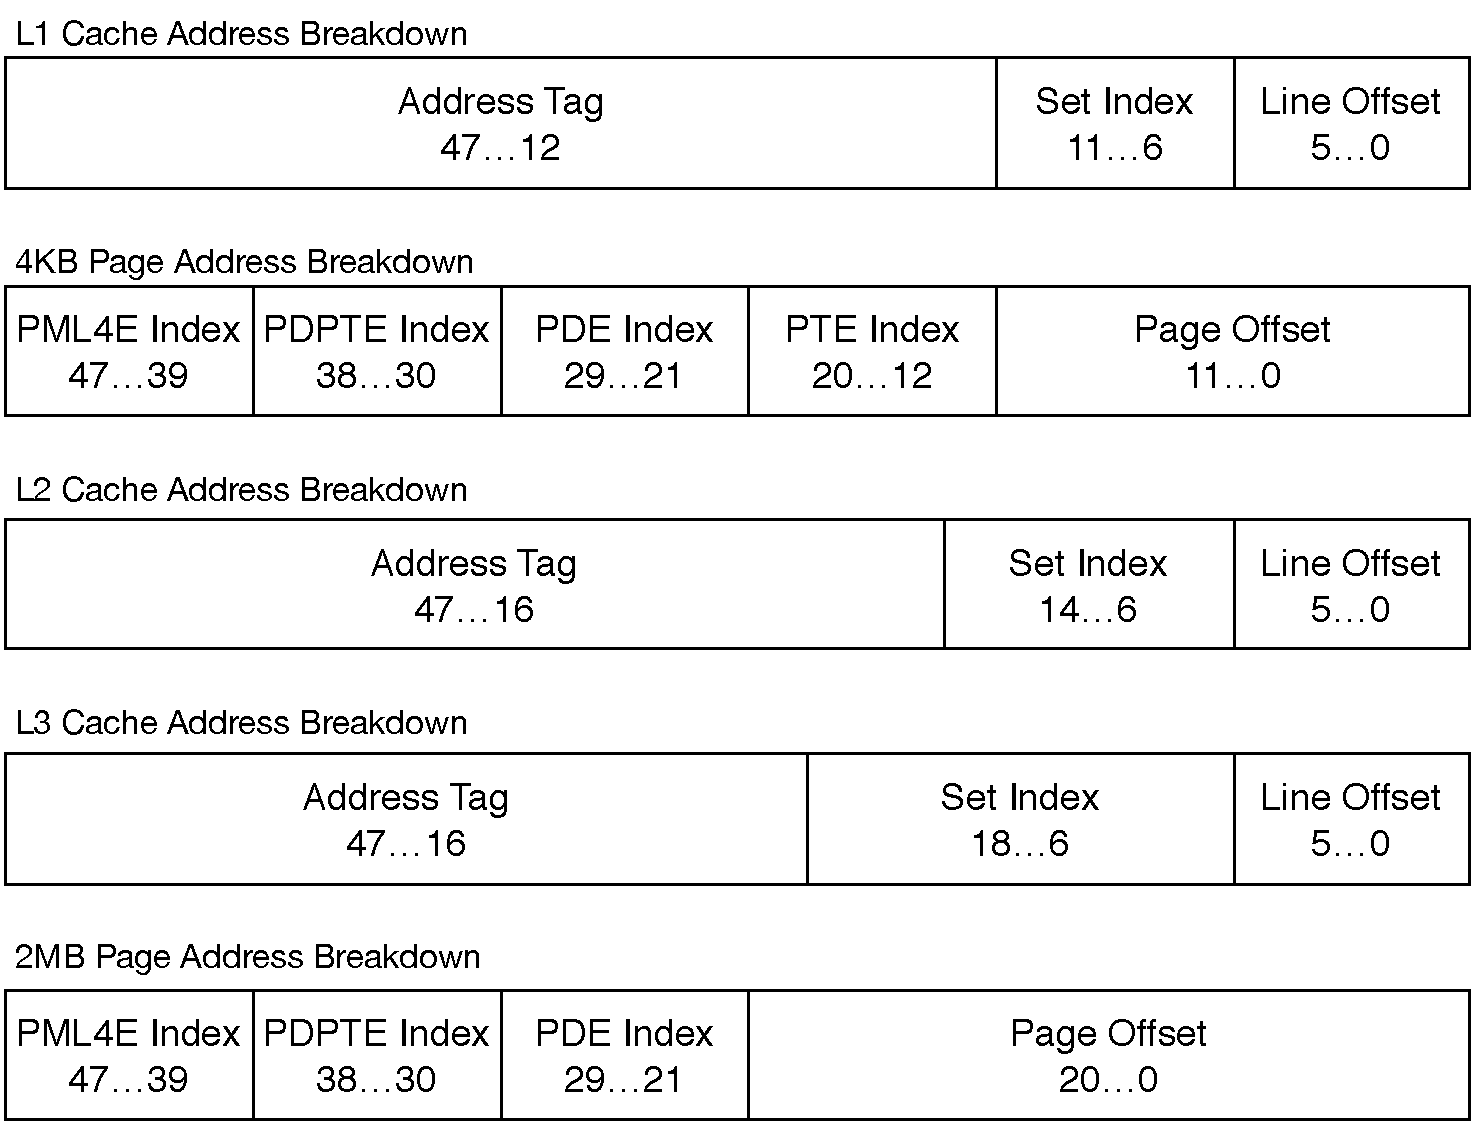
\includegraphics[width=85mm]{figures/caching_and_paging.pdf}}
  \caption{
    Virtual addresses from the perspective of cache lookup and address
    translation. The bits used for the L1 set index and line offset are not
    changed by address translation, so the page tables do not impact L1 cache
    placement. Page tables do impact L2 and L3 cache placement. Using large
    pages (2MB or 1GB) makes cache placement independent of page tables.
  }
  \label{fig:caching_and_paging}
\end{figure}

The L2 cache in recent Intel processors uses physical indexing
\cite{patterson2013architecture}. The indexing method is not documented in
Intel's manuals and is not reported by the CPUID instruction, as it is
considered to be an implementation detail. However, the indexing method
determines the set index for a given memory location, and knowing which memory
addresses are stored in the same set is crucial for mounting and defending
against cache timing attacks.

\begin{figure}[hbt]
  \center{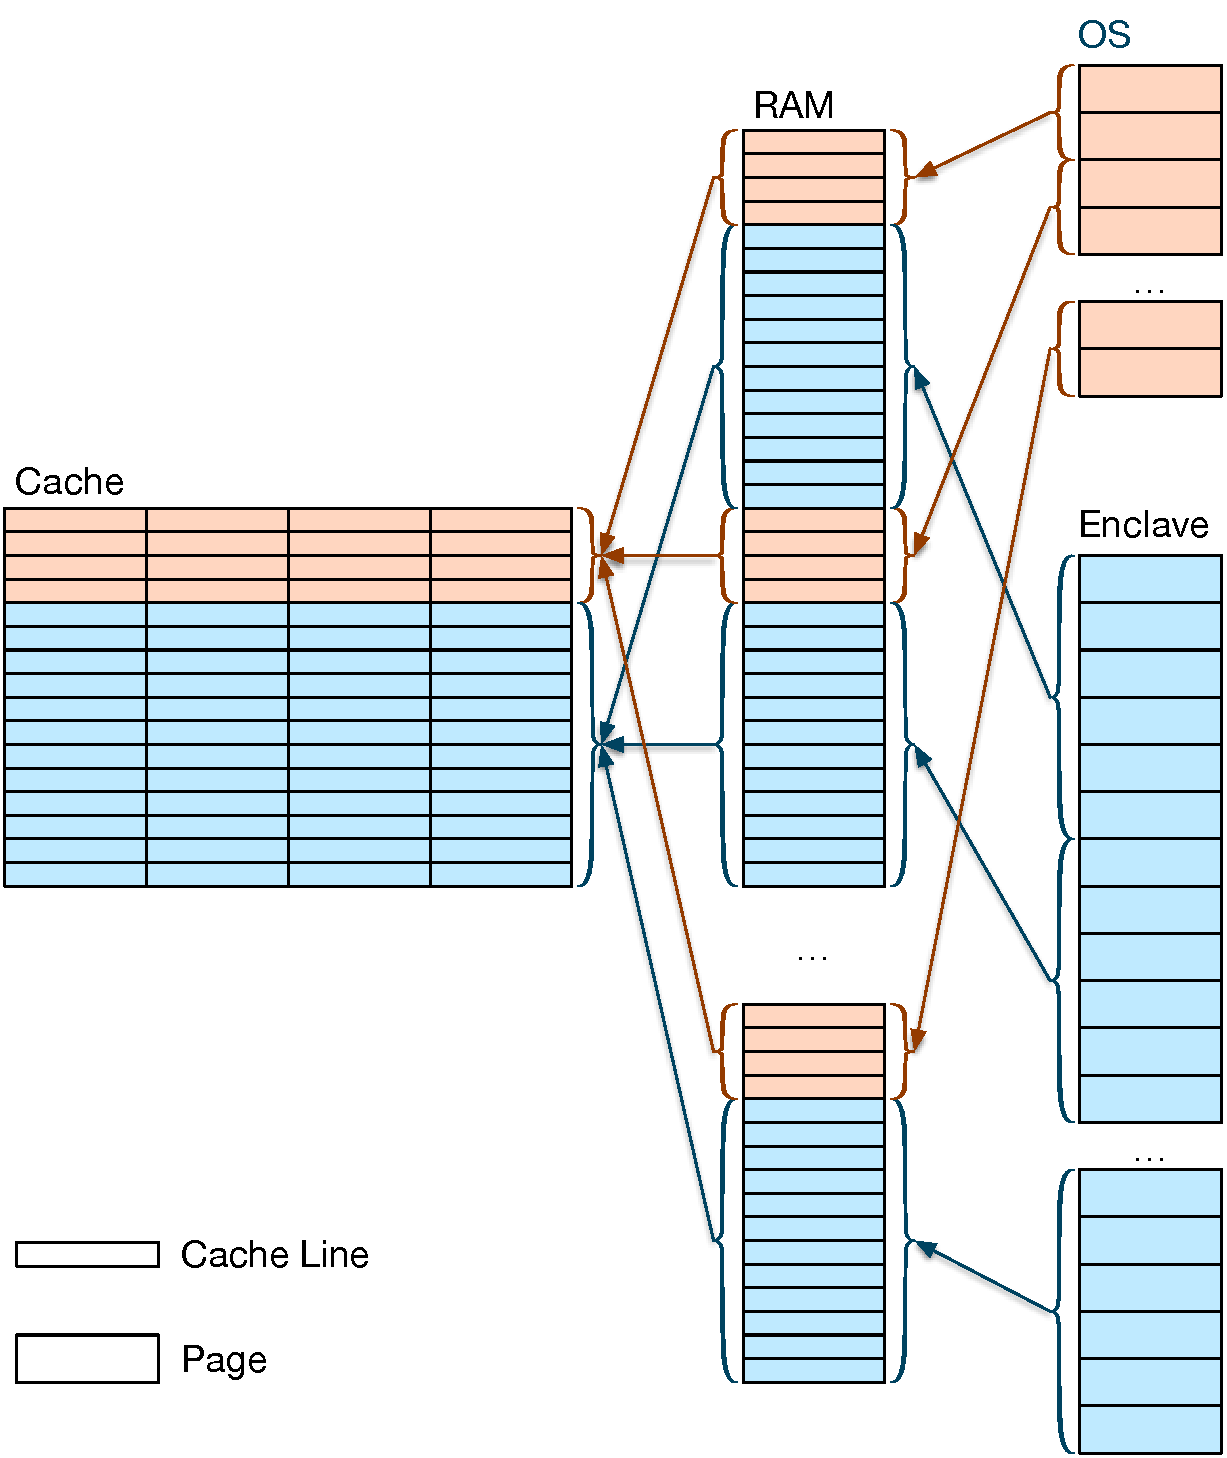
\includegraphics[width=85mm]{figures/cache_partitions.pdf}}
  \caption{
    Cache partitioning between two applications. Each application has some
    cache sets allocated to it, and only uses RAM regions that map to its cache
    sets. When partitioning the L1 cache, applications have to follow this
    constraint themselves. When the L2 cache is partitioned, the OS can map the
    pages in an application's virtual address space to the RAM regions that the
    application can use, so applications are oblivious to the cache
    partitioning.
  }
  \label{fig:cache_partitions}
\end{figure}

The system software is responsible for invalidating TLBs when it changes the
page tables that it manages. The Intel architecture has instructions that can
be used by the kernel and hypervisor to invalidate the TLB entries covering a
specific linear address. Some instructions invalidate all the TLB entries as a
side-effect.


\subsection{Caching and Logical Processors}
\label{sec:cache_coherence}

Intel's SDM describes the ordering guarantees that a software developer can
rely on when accessing the same memory location in multiple hardware threads.
The memory model is a variation on the Total Store Order (TSO) model
\cite{owens2009tso}, meaning that all the hardware threads will see the same
order of writes.

When the hardware threads that access the same memory location execute on
different cores, they may cause the cache line containing the memory location
to be loaded in each core's L1 and L2 cache. In order to provide TSO guarantees
in these circumstances, the processor cores use a \textit{cache coherence
protocol} that keeps the cache line copies in sync.

% Propagation of Paging-Structure Changes to Multiple Processors: SDM S 4.10.5

The cache coherence does not cover TLB entries. When modifying a page table
or EPT, the kernel and hypervisor are responsible for performing a
\textit{TLB shootdown}, which consists of stopping all the logical processors
that use the page table / EPT about to be changed, performing the changes,
executing TLB-invalidating instructions on the stopped logical processors, and
then resuming execution on the stopped logical processors.

\cite{hennessy2012architecture} provides a good introduction to cache coherence
principles. Intel's optimization reference \cite{intel2014optimization} states
that the coherence protocol used in Intel processors is
MESIF \cite{goodman2009mesif}, a variant of MESI.


\subsection{The Memory Subsystem}
\label{sec:cpu_uncore}

According to Intel's patents, the SGX memory protection relies on special
entries in the \textit{Source Address Decoder} (SAD) and \textit{Target Address
Decoder} (TAD).  A thorough understanding of the memory hierarchy is required
in order to understand this aspect of the SGX implementation.

The QPI protocol layer defines the cache coherence protocol, which is a variant
of MESIF \cite{goodman2009mesif}, an extension of MESI. The QPI protocol
defines caching agents, which are connected to the last-level cache in a
processor, and home agents, which are connected to memory controllers. Cache
agents make requests to home agents for cache line data on cache misses, while
home agents keep track of cache line ownership, and obtain the cache line data
from other cache line agents, or from the memory controller. Each processor has
its own home agent and caching agents.

On recent Intel processors, most of the memory hierarchy is implemented on the
processor chip. The Intel documentation refers to these on-chip components as
\textit{the uncore}. The uncore structure is described in some processor
family datasheets \cite{intel2014datasheet,intel2010datasheet}, and in the
overview sections in Intel's uncore performance monitoring documentation
\cite{intel2014uncore, intel2012uncore, intel2010uncore}.

UBox - uncore configuration controller; master for reading and writing
physically distributed registers across the uncore using the message
channel; receives interrupts from system and dispatches them to the
appropriate core; system lock master (e.g. QPI bus lock)

CBox - last-level cache (LLC) coherence engine; the interface between a core
and a slice of the LLC; acts as the QPI cache agent for that slice of LLC;
CBoxes are co-located with cores and connected in a ring interconnect

The physical memory space is split up between CBoxes. The ``complex'' caching
algorithm mentioned in the Intel SDM includes a ``hashing'' step that maps a
physical address to a CBox, and thus a slice of the LLC.

Each CBox contains a Source Address Decoder (SAD), and the configurations of
all SADs in a core are identical, replicated by the UBox. The SAD takes in a
memory address and access type, and outputs a transaction type (coherent,
non-coherent, IO) and a node ID.

Home agent - contains the Target Address Decoder (TAD) and interfaces with a
memory controller; a CPU may contain multiple home agents, if it has multiple
memory contollers; the TAD maps a memory address to a specific DRAM channel,
implements logical channel address mapping and interleaving;


\section{Related Work}
\label{sec:related}

This section describes the broader picture of trusted hardware projects that
SGX belongs to. Table~\ref{fig:secure_processors} summarizes the security
properties of SGX and the other trusted hardware presented here.

\begin{table*}
  \centering
  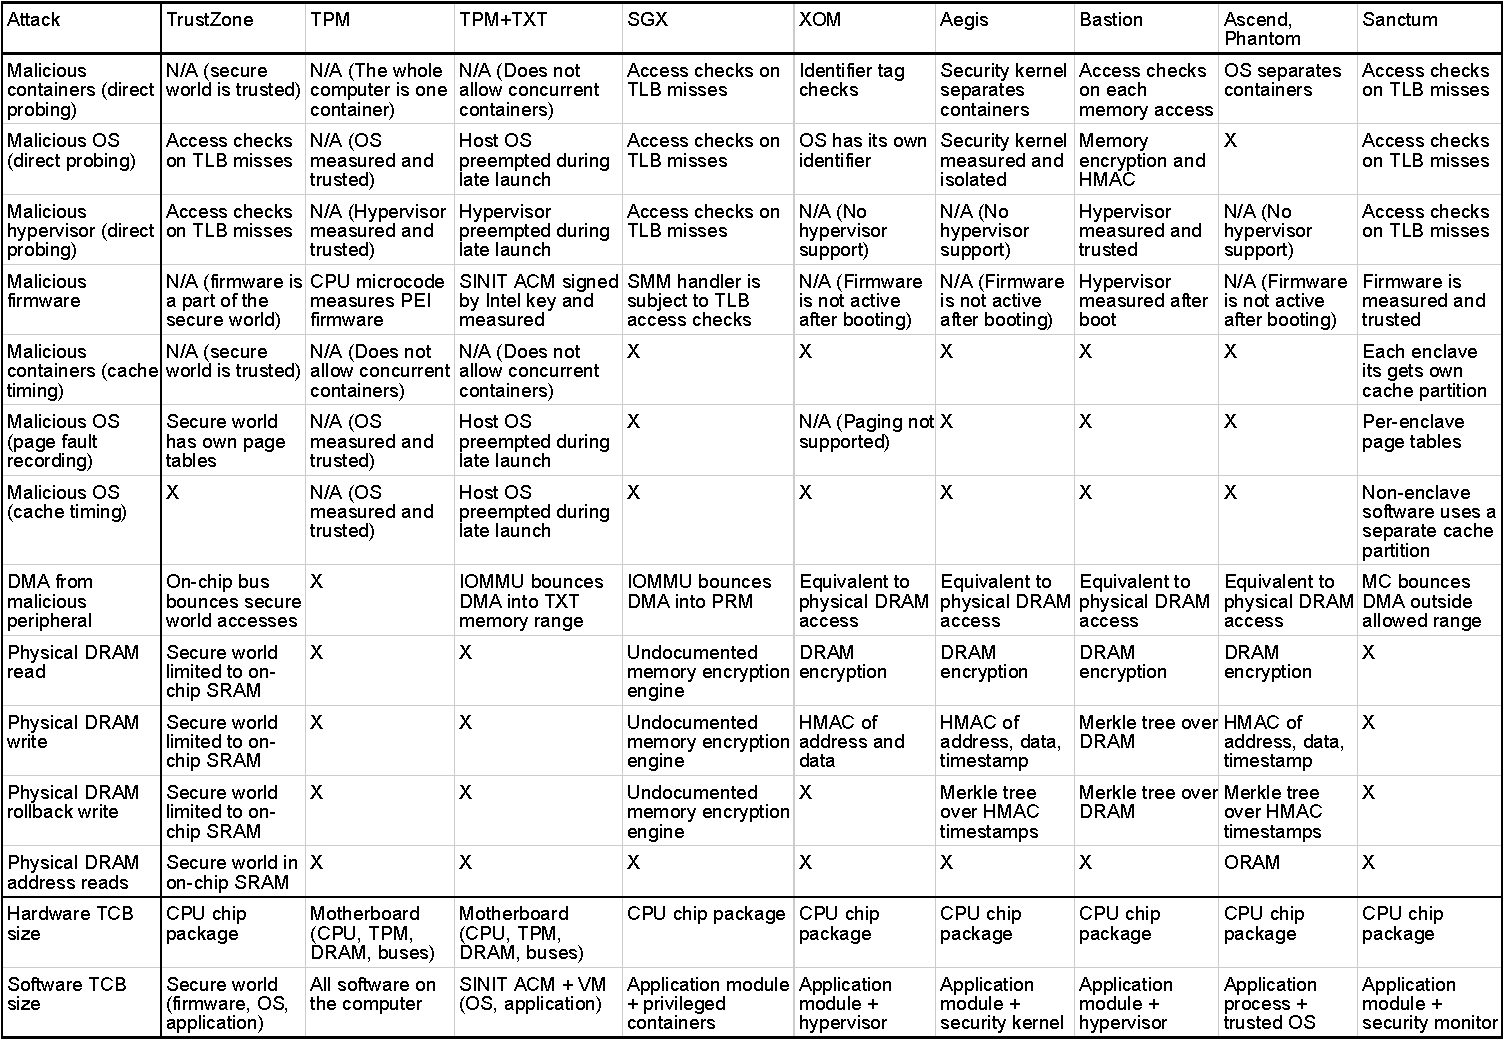
\includegraphics[angle=90,width=170mm]{figures/secure_processors_table.pdf}
  \caption{
    Security features overview for the trusted hardware projects related to
    Intel's SGX
  }
  \label{fig:secure_processors}
\end{table*}


\subsection{The IBM 4765 Secure Coprocessor}

Secure coprocessors~\cite{yee1994coprocessors} encapsulate an entire computer
system, including a CPU, a cryptographic accelerator, caches, DRAM, and an I/O
controller within a tamper-resistant environment. The enclosure includes
hardware that deters attacks, such as a Faraday cage, as well as an array of
sensors that can detect tampering attempts. The secure coprocessor destroys the
secrets that it stores when an attack is detected. This approach has good
security properties against physical attacks, but tamper-resistant enclosures
are very expensive~\cite{anderson2001security}, relatively to the cost of a
computer system.

The IBM 4758~\cite{smith1999ibm4758}, and its most current-day successor, the
IBM 4765~\cite{nist2015ibm4765} (shown in Figure~\ref{fig:ibm_4765}) are
representative examples of secure coprocessors. The 4758 was certified to
withstand physical attacks to FIPS 140-1 Level 4~\cite{smith1999validating},
and the 4765 meets the rigors of FIPS 140-2 Level 4~\cite{nist2011fipscert}.

\begin{figure}[hbt]
  \centering
  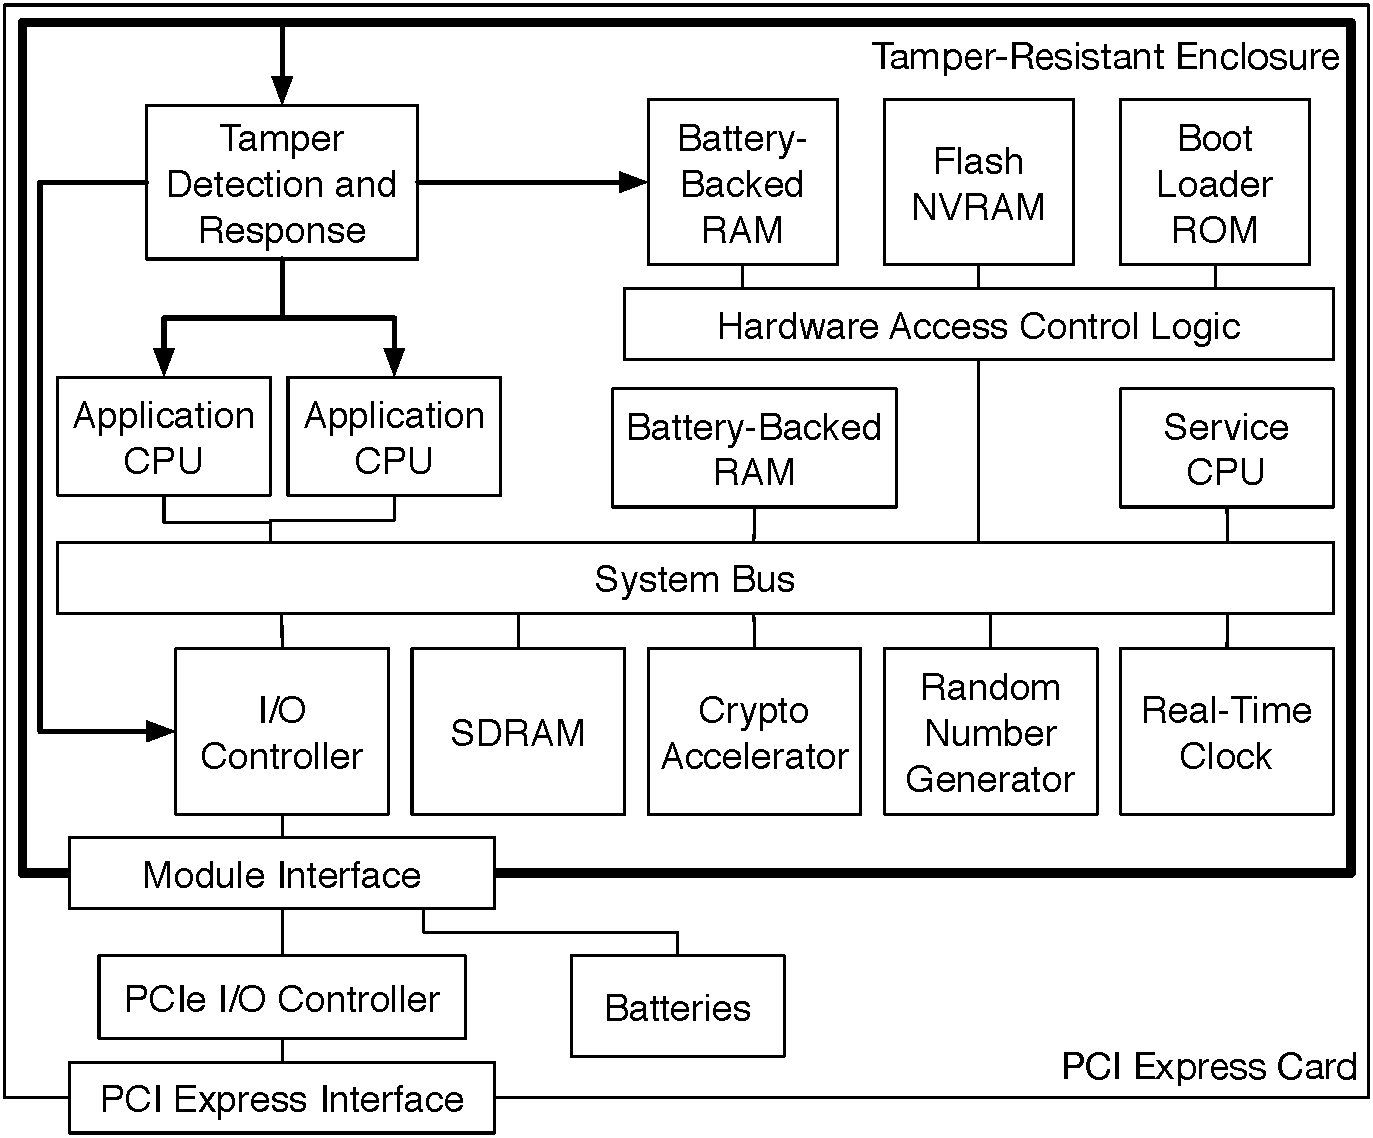
\includegraphics[width=85mm]{figures/ibm_4765.pdf}
  \caption{
    The IBM 4765 secure coprocessor consists of an entire computer system
    placed inside an enclosure that can deter and detect physical attacks.
    The application and the system use separate processors. Sensitive memory
    can only be accessed by the system code, thanks to access control checks
    implemented in the system bus' hardware. Dedicated hardware is used to clear
    the platform's secrets and shut down the system when a physical attack is
    detected.
  }
  \label{fig:ibm_4765}
\end{figure}

The 4765 relies heavily on physical isolation for its security properties. Its
system software is protected from attacks by the application software by
virtue of using a dedicated service processor that is completely separate from
the application processor. Special-purpose bus logic prevents the application
processor from accessing privileged resources, such as the battery-backed
memory that stores the system software's secrets.

The 4765 implements software attestation. The coprocessor's attestation key is
stored in battery-backed memory that is only accessible by the service
processor. Upon reset, the service processor executes a first-stage bootloader
stored in ROM, which measures and loads the system software. In turn, the
system software measures the application code stored in NVRAM and loads it into
the DRAM chip accessible to the application processor. The system software
provides attestation services to the application loaded inside the coprocessor.

\subsection{ARM TrustZone}

ARM's TrustZone~\cite{alves2004trustzone} is a collection of hardware modules
that can be used to conceptually partition a system's resources between a
\textit{secure world}, which hosts a secure container, and a \textit{normal
world}, which runs an untrusted software stack. The TrustZone
documentation~\cite{arm2009trustzone} describes semiconductor intellectual
property cores (IP blocks) and ways in which they can be combined to achieve
certain security properties, reflecting the fact that ARM is an IP core
provider, not a chip manufacturer. Therefore, the mere presence of TrustZone IP
blocks in a system is not sufficient to determine whether the system is secure
under a specific threat model. Figure~\ref{fig:trustzone} illustrates a design
for a smartphone \textit{System-on-Chip} (SoC) design that uses TrustZone IP
blocks.

\begin{figure}[hbt]
  \centering
  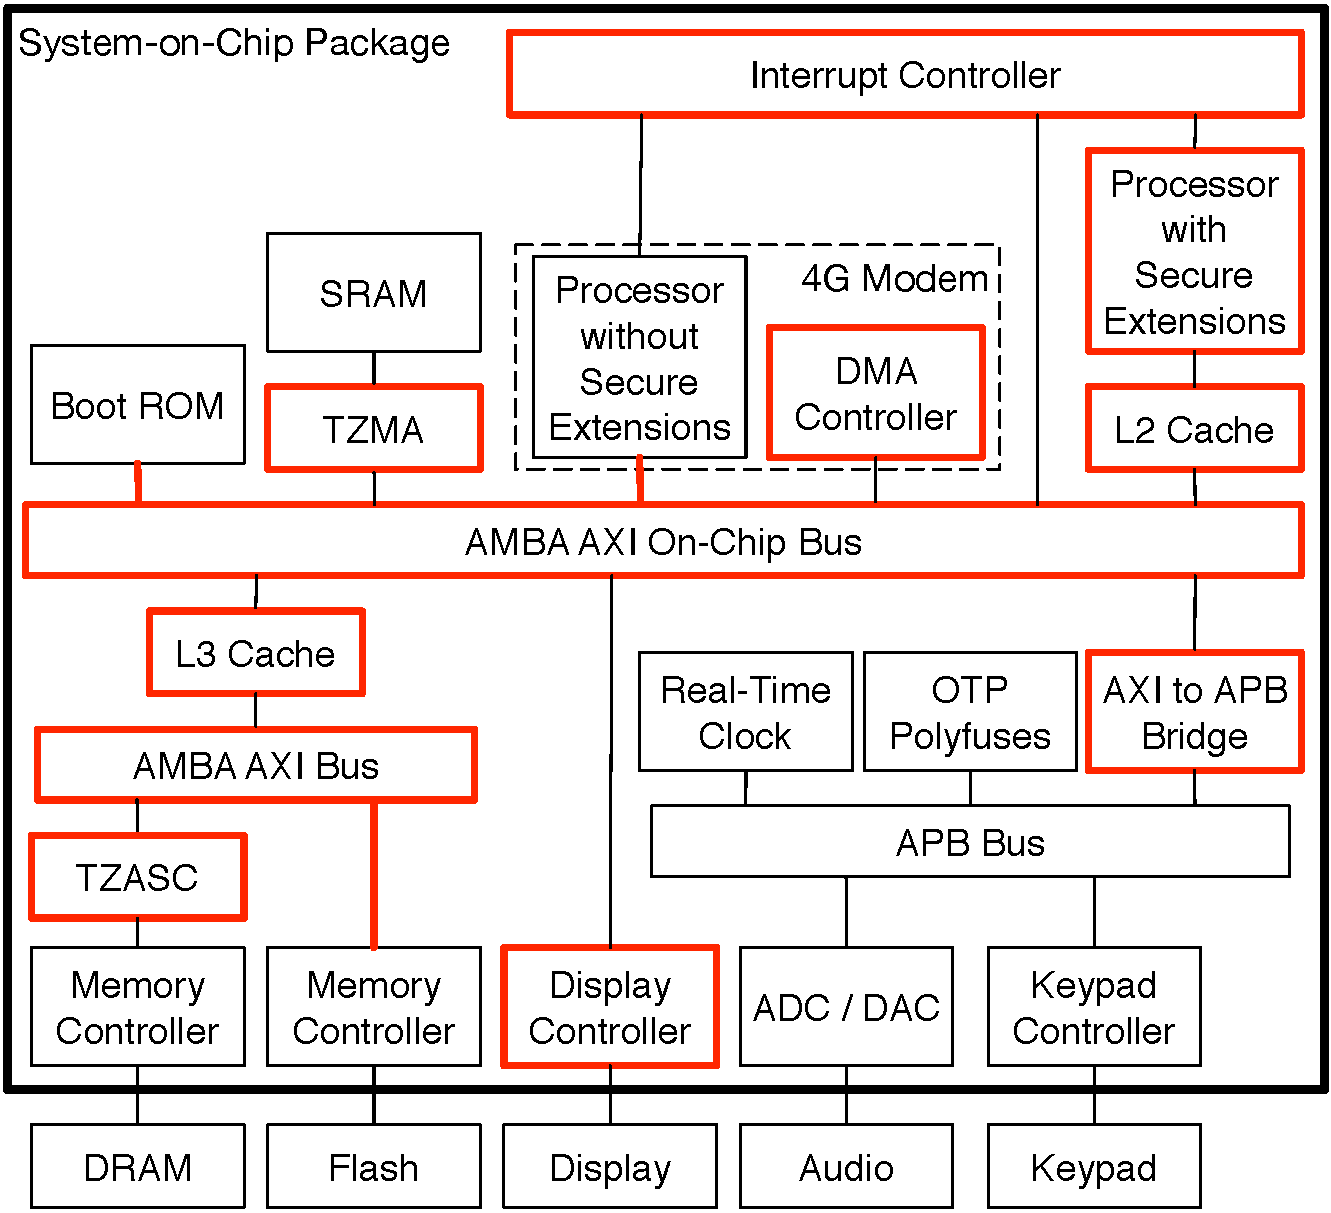
\includegraphics[width=85mm]{figures/trustzone.pdf}
  \caption{
    Smart SoC design based on TrustZone. The red IP blocks are TrustZone-aware.
    The red connections ignore the TrustZone secure bit in the bus address.
    Defining the system's security properties requires a complete understanding
    of all the red elements in this figure.
  }
  \label{fig:trustzone}
\end{figure}

TrustZone extends the address lines in the AMBA AXI system
bus~\cite{arm2004ambaxi} with one signal that indicates whether an access
belongs to the secure or normal (non-secure) world. ARM processor cores that
include TrustZone's ``Security Extensions'' can switch between executing code
in the normal world and code in the secure world. The address in each bus
access executed by a core reflects the world that the core is currently
executed.

The reset circuitry in a TrustZone processor places it in secure mode, and
points it to the first-stage bootloader stored in on-chip ROM. TrustZone's TCB
includes this bootloader, which initializes the platform, sets up the TrustZone
hardware to protect the secure container from untrusted software, and loads the
normal world's bootloader. The secure container must also implement a monitor
that performs the context switches needed to transition an execution core
between the two worlds. The monitor must also handle hardware exceptions, such
as interrupts, and route them to the appropriate world.

The TrustZone design gives the secure world's monitor unrestricted acces to the
normal world, so the monitor can implement inter-process communication (IPC)
between the software in the two worlds. Specifically, the monitor can issue
bus accesses using both secure and non-secure addresses. In general, the secure
world's software can compromise any level in the normal world's software stack.
For example, the secure container's software can jump into arbitrary locations
in the normal world by flipping a bit in a register. The untrusted software in
the normal world can only access the secure world via an instruction that jumps
into a well-defined location inside the monitor.

Conceptually, each TrustZone CPU core provides separate address translation
units for the secure and normal worlds. This is implemented by two page table
base registers, and by having the page walker use the page table base
corresponding to the core's current world. The physical addresses in the page
table entries are extended to include the values of the secure bit to be issued
on the AXI bus. The secure world is protected from untrusted software by having
the CPU core force the secure bit in the address translation result to zero for
normal world address translations. As the secure container manages its own page
tables, its memory accesses cannot be directly observed by the untrusted OS's
page fault handler.

TrustZone-aware hardware modules, such as caches, are trusted to use the secure
address bit in each bus access enforce the isolation between worlds. For
example, TrustZone's caches store the secure bit in the address tag for each
cache line, which effectively provides completely different views of the memory
space to the software running in different worlds. This design assumes that
memory space is partitioned between the two worlds, so no aliasing can occur.

The hardware modules that do not consume TrustZone's address bit are expected
to be connected to the AXI bus via IP cores that implement simple
partitioning techniques. For example, the TrustZone Memory Adapter (TZMA) can
be used to partition an on-chip ROM or SRAM into a secure region and a normal
region, and the TrustZone Address Space Controller (TZASC) partitions the
memory space provided by a DRAM controller into secure and normal regions. A
TrustZone-aware DMA controller rejects DMA transfers from the normal world that
reference secure world addresses.

It follows that analyzing the security properties of a TrustZone system
requires a precise understanding of the behavior and configuration of all the
hardware modules that are attached to the AXI bus. For example, the caches
described in TrustZone's documentation do not enforce a complete separation
between worlds, as they allow a world's memory accesses to evict the other
world's cache lines. This exposes the secure container software to cache timing
attacks from the untrusted software in the normal world. Unfortunately,
hardware manufacturers that license the TrustZone IP cores are reluctant to
disclose all the details of their designs, making it impossible for security
researchers to reason about TrustZone-based hardware.

The TrustZone components do not have any counter-measures for physical attacks.
However, a system that follows the recommendations in the TrustZone
documentation will not be exposed to physical attacks, under a threat model
that trusts the processor chip package. The AXI bus is designed to connect
components in a SoC design, so it cannot be tapped by an attacker. The
TrustZone documentation recommends having all the code and data in the secure
world stored in on-chip SRAM, which is not subjected to physical attacks.
However, this approach places significant limits on the secure container's
functionality, because on-chip SRAM is many orders of magnitude more expensive
than a DRAM chip of the same capacity.

TrustZone's documentation does not describe any software attestation
implementation. However, it does outline a method for implementing secure boot,
which comes down to having the first-stage bootloader verify a signature in the
second-stage bootloader against a public key whose cryptographic hash is burned
into on-chip \textit{One-Time Programmable} (OTP) polysilicon fuses. A hardware
measurement root can be built on top of the same components, by storing a
per-chip attestation key in the polyfuses, and having the first-stage
bootloader measure the second-stage bootloader and store its hash in an on-chip
SRAM region allocated to the secure world. The polyfuses would be gated by a
TZMA IP block that only makes them accessible to the secure world.

\HeadingLevelB{The XOM Architecture}

The execute-only memory (XOM) architecture \cite{lie2000xom} introduced the
approach of executing sensitive code and data in isolated containers managed by
untrusted host software. XOM outlined the mechanisms needed to isolate a
container's data from its untrusted software environment, such as saving the
register state to a protected memory area before servicing an interrupt.

XOM supports multiple containers by tagging every cache line with the
identifier of the container owning it, and ensures isolation by disallowing
memory accesses to cache lines that don't match the current container's
identifier. The operating system and the untrusted applications are considered
to belong to a container with a null identifier.

XOM also introduced the integration of encryption and HMAC functionality in
the processor's memory controller to protect container memory from physical
attacks on DRAM. The encryption and HMAC functionality is used for all cache
line evictions and fetches, and the ECC bits in DRAM chips are repurposed to
store HMAC values.

XOM's design cannot guarantee DRAM freshness, so the software in its containers
is vulnerable to physical replay attacks. Furthermore, XOM does not protect a
container's memory access patterns, meaning that any piece of malicious
software can perform cache timing attacks against the software in a container.
Last, XOM containers are destroyed when they encounter hardware exceptions,
such as page faults, so XOM does not support paging.

XOM predates the attestation scheme described above, and relies on a modified
software distribution scheme instead. Each container's contents are encrypted
with a symmetric key, which also serves as the container's identity. The
symmetric key, in turn, is encrypted with the public key of each CPU that is
trusted to run the container. A container's author can be assured that the
container is running on trusted software by embedding a secret into the
encrypted container data, and using it to authenticate the container. While
conceptually simpler than software attestation, this scheme does not allow the
container author to vet the container's software environment.

\HeadingLevelB{The Trusted Platform Module (TPM)}
\label{sec:sgx_related_tpm}

The Trusted Platform Module (TPM) \cite{grawrock2003tpm} introduced the
software attestation model described at the beginning of this section. The TPM
design does not require any hardware modifications to the CPU, and instead
relies on an auxiliary tamper-resistant chip. The TPM chip is only used to
store the attestation key and to perform software attestation. The TPM was
widely deployed on commodity computers, because it does not rely on CPU
modifications. Unfortunately, the cost of this approach is that the TPM has
very weak security guarantees, as explained below.

The TPM design provides one isolation container, covering all the software
running on the computer that has the TPM chip. It follows that the measurement
included in an attestation signature covers the entire OS kernel and all the
kernel modules, such as device drivers. However, commercial computers use a
wide diversity of devices, and their system software is updated at an
ever-increasing pace, so it is impossible to maintain a list of acceptable
measurement hashes corresponding to a piece of trusted software. Due to this
issue, the TPM's software attestation is not used in many security systems,
despite its wide deployment.

The TPM design is technically not vulnerable to any software attacks, because
it trusts all the software on the computer. However, a TPM-based system is
vulnerable to an attacker who has physical access to the machine, as the TPM
chip does not provide any isolation for the software on the computer.
Furthermore, the TPM chip receives the software measurements from the CPU,
so TPM-based systems are vulnerable to attackers who can tap the communication
bus between the CPU and the TPM.

Last, the TPM's design relies on the software running on the CPU to report its
own cryptographic hash. The TPM chip resets the measurements stored in Platform
Configuration Registers (PCRs) when the computer is rebooted. Then, the TPM
expects the software at each boot stage to cryptographically hash the software
at the next stage, and send the hash to the TPM. The TPM updates the PCRs to
incorporate the new hashes it receives, as shown in
Figure~\ref{fig:tpm_measurement}. Most importantly, the PCR value at any point
reflects all the software hashes received by the TPM up to that point. This
makes it impossible for software that has been measured to ``remove'' itself
from the measurement.

\begin{figure}[hbt]
  \centering
  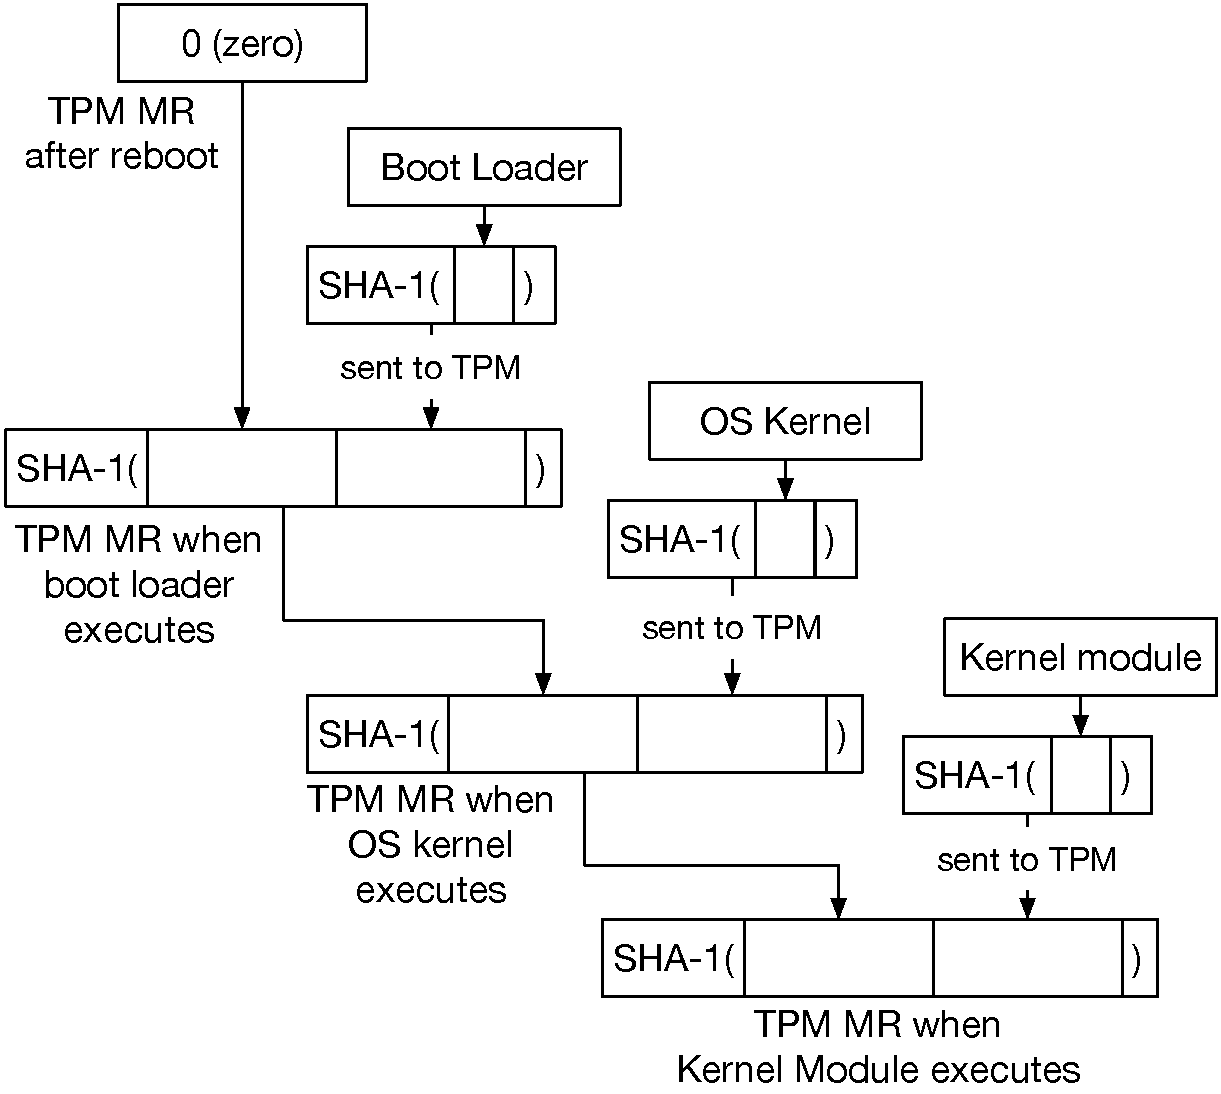
\includegraphics[width=85mm]{figures/tpm_measurement.pdf}
  \caption{
    The measurement stored in a TPM platform configuration register (PCR). The
    PCR is reset when the system reboots. The software at every boot stage
    hashes the next boot stage, and sends the hash to the TPM. The PCR's new
    value incorporates both the old PCR value, and the new software hash.
  }
  \label{fig:tpm_measurement}
\end{figure}

For example, the firmware on most modern computers implements the platform
initialization process in the Unified Extensible Firmware Interface (UEFI)
specification~\cite{forum2015uefi}. Each platform initialization phase is
responsible for verifying or measuring the firmware that implements the next
phase. The SEC firmware initializes the TPM PCR, and then stores the PEI's
measurement into a measurement register. In turn, the PEI implementation
measures the DXE firmware and updates the measurement register that stores the
PEI hash to account for the DXE hash. When the OS is booted, the hash in the
measurement register accounts for all the firmware that was used to boot the
computer.

Unfortunately, the security of the whole measurement scheme hinges on the
requirement that the first hash sent to the TPM must reflect the software that
runs in the first boot stage. The TPM threat model explicitly acknowledges this
issue, and assumes that the firmware responsible for loading the first stage
bootloader is securely embedded in the motherboard. However, virtually every
TPM-enabled computer stores its firmware in a flash memory chip that can be
re-programmed in software (\S~\ref{sec:motherboard}), so the TPM's measurement
can be subverted by an attacker who can reflash the computer's firmware
\cite{butterworth2013bios}.

On very recent Intel processors, the attack described above can be defeated by
having the initialization microcode (\S~\ref{sec:microcode_sec}) hash the
computer's firmware (specifically, the PEI code in UEFI \cite{forum2015uefi}
firwmare) and communicate the hash to the TPM chip. This is marketed as the
Measured Boot feature of Intel's Boot Guard \cite{ruan2014intelme}.

Sadly, most computer manufacturers use Verified Boot (also known as ``secure
boot'') instead of Measured Boot (also known as ``trusted boot''). Verified
Boot means that the processor's microcode only boots into PEI firmware that
contains a signature produced by a key burned into the chip's e-fuses. Verified
Boot does not impact the measurements stored on the TPM, so it does not improve
the security of software attestation.

\subsection{Intel's Trusted Execution Technology (TXT)}

Intel's Trusted Execution Technology (TXT) \cite{grawrock2009txt} uses the
TPM's software attestation model and auxilliary tamper-resistant chip, but
reduces the software inside the secure container to a virtual machine (guest
operating system and application) hosted by the CPU's hardware virtualization
features (VMX \cite{uhlig2005vmx}).

TXT isolates the software inside the container from untrusted software by
ensuring that the container has exclusive control over the entire computer
while it is active. This is accomplished by a secure initialization
authenticated code module (SINIT ACM) that effectively performs a warm system
reset before starting the container's VM.

TXT does not implement DRAM encryption or HMACs, and therefore is vulnerable to
physical DRAM attacks, just like TPM-based designs. Furthermore, early TXT
implementations were vulnerable to attacks where a malicious operating system
would program a device, such as a network card, to perform DMA transfers
to the DRAM region used by a TXT container \cite{wojtczuk2009txt,
wojtczuk2009txt2}. In recent Intel CPUs, the memory controller is integrated on
the CPU die, so the SINIT ACM
can securely set up the memory controller to reject DMA transfers targeting TXT
memory.

Early TXT implementations did not measure the SINIT ACM. Instead, the microcode
implementing the TXT launch instruction verified that the code module contained
an RSA signature by a hard-coded Intel key. SINIT ACM signatures cannot be
revoked if vulnerabilities are found, so TXT's software attestation had to be
revised when SINIT ACM exploits \cite{wojtczuk2011txt} surfaced. Currently, the
SINIT ACM's cryptographic hash is included in the attestation measurement.

Last, the warm reset performed by the SINIT ACM does not include the software
running in System Management Mode (SMM). SMM was designed
solely for the use of firmware, and is stored in a protected memory area
(SMRAM) which should not be accessible to non-SMM software. However, the SMM
handler was compromised on multiple occasions \cite{duflot2006smm,
rutkowska2008remap, wojtczuk2009smm, wecherowski2009smm, embleton2010smm}, and
an attacker that obtains SMM execution can access the memory used by TXT's
container.

\subsection{The Aegis Secure Processor}

The Aegis secure processor \cite{suh2003aegis} argued that Physically
Uncloneable Functions (PUFs) \cite{gassend2002puf} can be used to endow a
secure processor with a tamper-resistant private key, which is required for
software attestation. PUFs do not have the fabrication process drawbacks of
EEPROM, and are significantly more resilient to physical attacks than e-fuses.
Aegis relies on a security kernel in the operating system to isolate
containers, and includes the kernel's cryptographic hash in the measurement
reported by the software attestation signature.

Aegis relies on a trusted security kernel to isolate each container from the
other software on the computer by configuring the page tables used in address
translation. The security kernel is a subset of a typical OS kernel, and
handles virtual memory management, processes, and hardware exceptions. As the
security kernel is a part of the \textit{trusted code base} (TCB), its
cryptographic hash is included in the software attestation measurement. The
security kernel uses processor features to isolate itself from the untrusted
part of the operatings system, such as device drivers.

The Aegis memory controller encrypts the cache lines in one memory range, and
HMACs the cache lines in one other memory range. The two memory ranges can
overlap, and are configurable by the security kernel. Thanks to the two ranges,
the memory controller can avoid the latency overhead of cryptographic
operations for the DRAM outside containers. Aegis is not vulnerable to physical
replay attacks, as it uses a Merkle tree construction \cite{gassend2003merkle}
to guarantee DRAM freshness. The latency overhead of the Merkle tree is greatly
reduced by augmenting the L2 cache with the tree nodes for the cache lines.

Aegis' security kernel allows the OS to page out container memory, but verifies
the correctness of the paging operations. The security kernel uses the same
encryption and Merkle tree algorithms as the memory controller to guarantee the
privacy and integrity of the container pages that are swapped out from DRAM.
As the OS is free to page out container memory, it can learn a containter's
memory access patterns, at page granularity. Aegis containers are also
vulnerable to cache timing attacks.

\HeadingLevelB{The Bastion Architecture}
\label{sec:sgx_related_bastion}

The Bastion architecture \cite{champagne2010bastion} introduced the use of a
trusted hypervisor to provide secure containers to applications running inside
unmodified, untrusted operating systems. Bastion's hypervisor ensures that the
operating system does not interfere with the secure containers. We only
describe Bastion's virtualization extensions to architectures that use nested
page tables, like Intel's VMX \cite{uhlig2005vmx}.

The hypervisor enforces the containers' desired memory mappings in the OS page
tables, as follows. Each Bastion container has a Security Segment that lists
the virtual addresses and permissions of all the container's pages, and the
hypervisor maintains a Module State Table that stores an inverted page map,
associating each physical memory page to its container and virtual address. The
processor's hardware page walker is modified to invoke the hypervisor on every
TLB miss, before updating the TLB with the address translation result. The
hypervisor checks that the virtual address used by the translation matches the
expected virtual address associated with the physical address in the Module
State Table.

Bastion's cache lines are not tagged with container identifiers. Instead, only
TLB entries are tagged. The hypervisor's TLB miss handler sets the container
identifier for each TLB entry as it is created. Similarly to XOM and Aegis, the
secure processor checks the TLB tag against the current container's identifier
on every memory access.

Bastion offers the same protection against physical DRAM attacks as Aegis does,
without the restriction that a container's data must be stored inside a
continuous DRAM range. This is accomplished by extending cache lines and TLB
entries with flags that enable memory encryption and HMACing. The hypervisor's
TLB miss handler sets the flags on TLB entries, and the flags are propagated to
cache lines on memory writes.

The Bastion hypervisor allows the untrusted operating system to evict secure
container pages. The evicted pages are encrypted, HMACed, and covered by a
Merkle tree maintained by the hypervisor. Thus, the hypervisor ensures the
privacy, authenticity, and freshness of the swapped pages. However, the ability
to freely evict container pages allows a malicious OS to learn a container's
memory accesses with page granularity. Furthermore, Bastion's threat model
excludes cache timing attacks.

Bastion does not trust the platform's firmware, and computes the cryptographic
hash of the hypervisor after the firmware finishes playing its part in the
booting process. The hypervisor's hash is included in the measurement reported
by software attestation.

Intel's Software Guard Extensions (SGX)~\cite{mckeen2013sgx, anati2013sgx,
hoekstra2013sgx} implements secure containers for applications without making
any modifications to the processor's critical execution path. SGX does not
trust any layer in the computer's software stack (firmware, hypervisor, OS).
Instead, SGX's TCB consists of the CPU's microcode and a few privileged
containers. SGX introduces an approach to solving some of the issues raised by
multi-core processors with a shared, coherent last-level cache.

SGX does not extend caches or TLBs with container identity bits, and does not
require any security checks during normal memory accesses. As suggested in the
TrustZone documentation, SGX always ensures that a core's TLBs only contain
entries for the container that it is executing, which requires flushing the CPU
core's TLBs when context-switching between containers and untrusted software.

SGX follows Bastion's approach of having the untrusted OS manage the page
tables used by secure containers. The containers' security is preserved by a
TLB miss handler that relies on an inverted page map (the EPCM) to reject
address translations for memory that does not belong to the current container.

Like Bastion, SGX allows the untrusted operating system to evict secure
container pages, in a controlled fashion. After the OS initiates a container
page eviction, it must prove to the SGX implementation that it also switched
the container out of all cores that were executing its code, effectively
performing a very coarse-grained TLB shootdown.

SGX's microcode ensures the confidentiality, authenticity, and freshness of
each container's evicted pages, like Bastion's hypervisor. However, SGX relies
on a version-based Merkle tree, inspired by Aegis \cite{suh2003aegis}, and adds
an innovative twist that allows the operating system to dynamically shape the
Merkle tree. SGX also shares Bastion's and Aegis' vulnerability to memory
access pattern leaks, namely a malicious OS can directly learn a container's
memory accesses at page granularity, and any piece of software can perform
cache timing attacks.

SGX's software attestation is implemented using Intel's Enhanced Privacy ID
(EPID) group signature scheme \cite{brickell2009epid}, which is too complex for
a microcode implementation. Therefore, SGX relies on an assortment of
privileged containers that receive direct access to the SGX processor's
hardware keys. The privileged containers are signed using an Intel private key
whose corresponding public key is hard-coded into the SGX microcode, similarly
to TXT's SINIT ACM.

As SGX does not protect against cache timing attacks, the privileged enclave's
authors cannot use data-dependent memory accesses. For example, cache attacks
on the Quoting Enclave, which computes attestation signatures, would provide
an attack with a processor's EPID signing key and completely compromise SGX.

Intel's documentation states that SGX guarantees DRAM confidentiality,
authentication, and freshness by virtue of a Memory Encryption Engine (MEE).
The MEE is informally described in an ISCA 2015
tutorial~\cite{intel2015iscasgx}, and appears to lack a formal specification.
In the absence of further information, we assume that SGX provides the same
protection against physical DRAM attacks that Aegis and Bastion provide.

\HeadingLevelB{Sanctum}
\label{sec:related_sanctum}

Sanctum~\cite{costan2015sanctum} introduced a straightforward software/hardware
co-design that yields the same resilience against software attacks as SGX, and
adds protection against memory access pattern leaks, such as page fault
monitoring attacks and cache timing attacks.

Sanctum uses a conceptually simple cache partitioning scheme, where a
computer's DRAM is split into equally-sized continuous DRAM regions, and each
DRAM region uses distinct sets in the shared last-level cache (LLC). Each DRAM
region is allocated to exactly one container, so containers are isolated in
both DRAM and the LLC. Containers are isolated in the other caches by flushing
on context switches.

Like XOM, Aegis, and Bastion, Sanctum also considers the hypervisor, OS, and the
application software to conceptually belong to a separate container. Containers
are protected from the untrusted outside software by the same measures that
isolate containers from each other.

Sanctum relies on a trusted security monitor, which is the first piece of
firmware executed by the processor, and has the same security properties as
those of Aegis' security kernel. The monitor is measured by bootstrap code in
the processor's ROM, and its cryptographic hash is included in the software
attestation measurement. The monitor verifies the operating system's resource
allocation decisions. For example, it ensures that no DRAM region is ever
accessible to two different containers.

Each Sanctum container manages its own page tables mapping its DRAM regions,
and handles its own page faults. It follows that a malicious OS cannot learn the
virtual addresses that would cause a page fault in the container. Sanctum's
hardware modifications work in conjunction with the security monitor to make
sure that a container's page tables only reference memory inside the container's
DRAM regions.

The Sanctum design focuses completely on software attacks, and does not offer
protection from any physical attack. The authors expect Sanctum's hardware
modifications to be combined with the physical attack protections in Aegis or
Ascend.

\HeadingLevelB{Ascend and Phantom}

The Ascend \cite{fletcher2012ascend} and Phantom \cite{maas2013phantom} secure
processors introduced practical implementations of Oblivious RAM
\cite{goldreich1987oram} techniques in the CPU's memory controller. These
processors are resilient to attackers who can probe the DRAM address bus and
attempt to learn a container's private information from its DRAM memory access
pattern.

Implementing an ORAM scheme in a memory controller is largely orthogonal to the
other secure architectures described above. It follows, for example, that
Ascend's ORAM implementation can be combined with Aegis' memory encryption and
authentication, and with Sanctum's hardware extensions and security monitor,
yielding a secure processor that can withstand both software attacks and
physical DRAM attacks.


\section{SGX Memory Organization}
\label{sec:memory}

The central concept of SGX is the \textit{enclave}, a protected environment
that contains the code and data pertaining to a security-sensitive computation.
This section provides an overview of the data structures used by an enclave.


\subsection{Enclaves in DRAM}
\label{sec:prm}

% Intel SGX Resource Enumeration Leaves: SDM S 37.7.2
% Interactions with DMA: SDM S 42.10, SGX2 S 6.10

The enclaves' code and data is stored in \textit{Processor Reserved Memory}
(PRM), which cannot be directly accessed by other software, including system
software and SMM code. The CPU's integrated memory controllers
(\S~\ref{sec:cpu_die}) also reject DMA transfers targeting the PRM, thus
protecting it from access by other peripherals.

\begin{figure}[hbt]
  \centering
  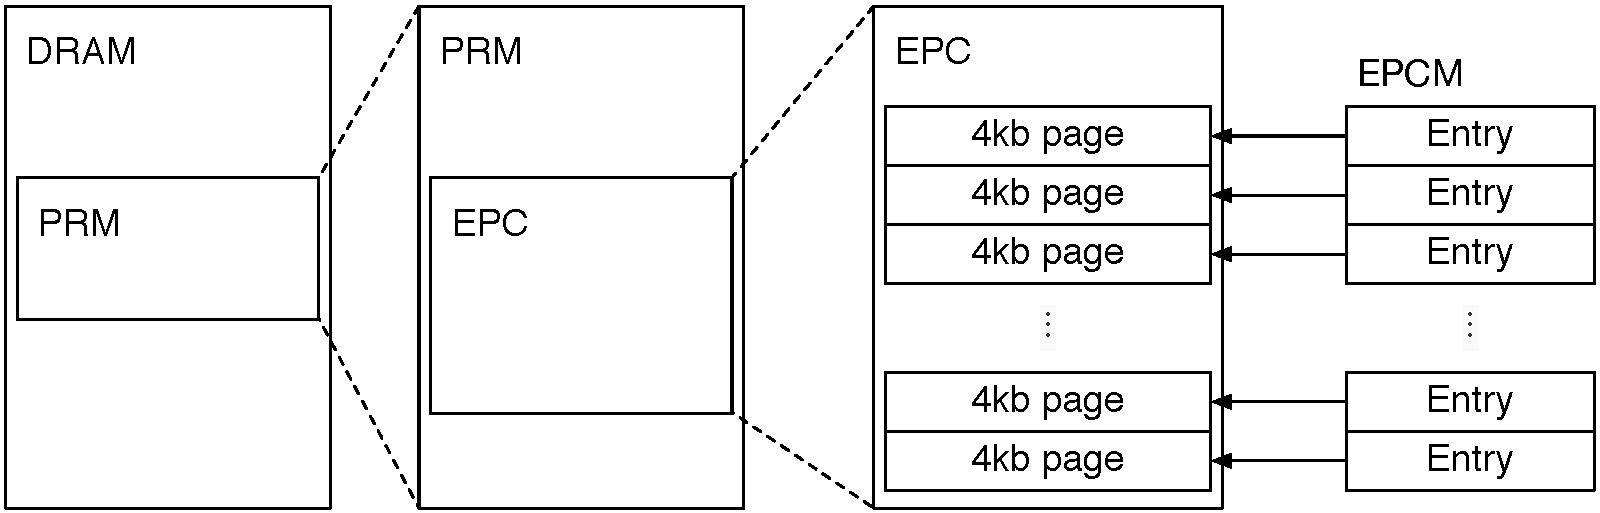
\includegraphics[width=87mm]{figures/sgx_epc.pdf}
  \caption{
    Enclave data is stored into the EPC, which is a subset of the PRM. The
    PRM is a contiguous range of DRAM that cannot be accessed by system
    software or peripherals.
  }
  \label{fig:sgx_epc}
\end{figure}

% EPC and Management of EPC Pages: SGX2 S 3.5
% Interactions with Memory Configuration: SGX2 S 6.11
% Memory Type Considerations for PRMRR: SGX2 S 6.11.1
% Interactions of PRMRR with Physical Memory Accesses: SGX2 S 6.11.3.1

The PRM range is configured using a base and a mask register with the same
semantics as a variable memory type range (\S~\ref{sec:cacheability_config}),
which implies that the PRM's size must be an integer power of two, and its
start address must be aligned to the same power of two. These restrictions make
it cheap to check if an address belongs to the PRM in hardware, as described in
\S~\ref{sec:cacheability_config}.

The PRM and PRM range registers (PRMRR) are described in the SGX
manuals~\cite{intel2013sgxmanual, intel2014sgx2manual} and in one of the SGX
papers~\cite{mckeen2013sgx}. The SDM mostly mirrors the SGX manuals, but lacks
most of the sections mentioning the PRM.


\subsubsection{The Enclave Page Cache (EPC)}
\label{sec:epc}

% Enclave Page Cache: SDM S 37.5
% EPC and Management of EPC Pages: SDM S 39.5, S 39.5.1

The contents of enclaves and the associated data structures are stored in the
\textit{Enclave Page Cache} (EPC), which is a subset of the PRM.

The SGX design supports having multiple enclaves on a system at the same time,
which is a  necessity in multi-process environments. This is achieved by having
the EPC split into 4~KB pages that can be associated to different enclaves. The
system software uses SGX instructions to allocate unused pages to enclaves, and
to free previously allocated EPC pages.

The SGX instructions that allocate an EPC page to an enclave also copy data
from a page outside PRM to the EPC page. Non-enclave software is not permitted
to access the PRM, so the page allocation instructions are the only avenue for
system software to load the initial code and data into an enclave.

SGX also offers a method for system software to evict EPC pages into non-PRM
memory, which allows the EPC to be over-committed, just like evicting DRAM
pages to disk (swapping) allows the main memory to be over-committed.


\subsubsection{Memory Mapping Attacks}
\label{sec:mapping_attacks}

% Access Control Requirements: SDM S 38.3

One of SGX's design goals is to make it easy to migrate the sensitive pieces of
an application into an enclave. To this end, enclave code uses the same address
translation process (\S~\ref{sec:paging}) as the application hosting the
enclave. It follows that enclave code can access non-EPC memory using the same
virtual addresses as the host application, which makes it easy to migrate
application code that uses pointers into SGX enclaves.

% Interactions with VMX: SDM S 42.5, S 42.5.{1,2,3,4,5}

Under SGX, the operating system and hypervisor are still in full control of the
page tables and EPTs. This minimizes the amount of changes required to add SGX
support to existing system software. However, it also gives system software the
ability to attack an enclave by setting up its virtual address space in a way
that was not intended by the enclave's author.

Figure~\ref{fig:sgx_mapping_attack} shows a hypothetical memory mapping attack
that is prevented by SGX's security measures. Understanding this type of attack
greatly increases one's ability to reason about SGX's security.

\begin{figure}[hbt]
  \centering
  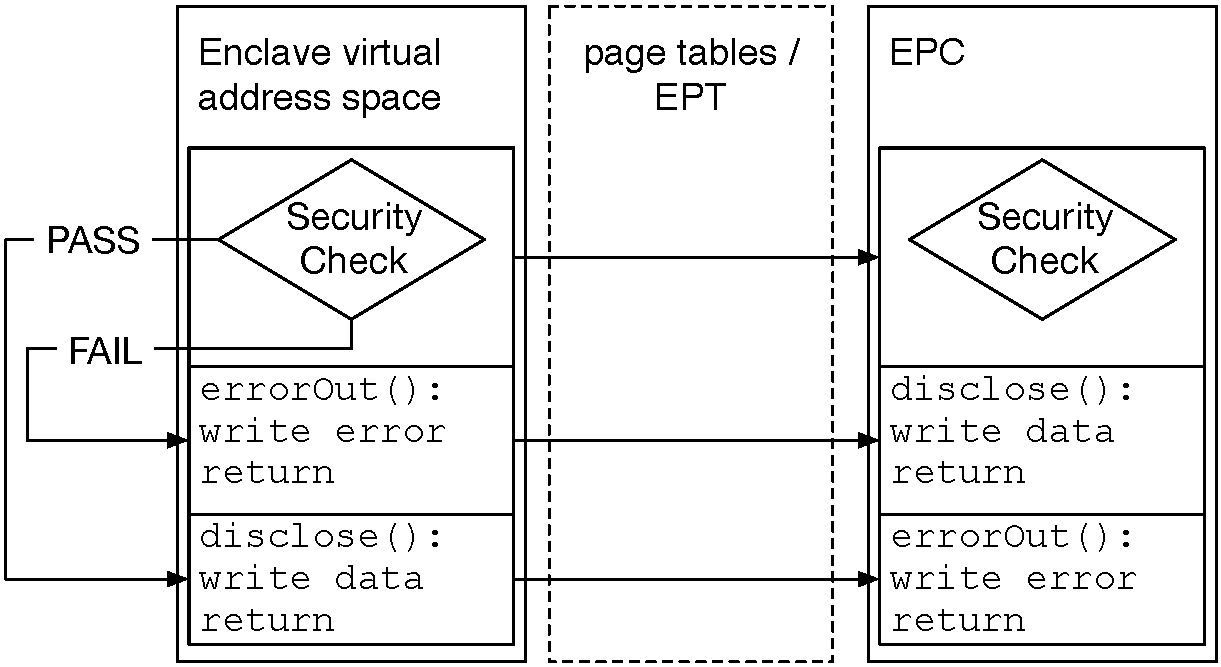
\includegraphics[width=85mm]{figures/sgx_mapping_attack.pdf}
  \caption{
    An example of a memory mapping attack, which is prevented by SGX. The
    enclave's author intends to disclose a piece of sensitive information only
    when a security check passes. Malicious system software maps the virtual
    address of the procedure called when the security check fails to an EPC
    page that contains the procedure that discloses the sensitive information,
    which is supposed to be called when the security check passes.
  }
  \label{fig:sgx_mapping_attack}
\end{figure}

For simplicity, we assume an enclave that performs a security check to decide
whether to disclose some sensitive information. Depending on the security
check's outcome, the enclave code either calls a \texttt{errorOut} procedure,
or a \texttt{disclose} procedure. We furthermore assume that each procedure's
code starts at a 4KB boundary, and takes up less than 4KB, so each procedure
fits in an EPC page. These requirements seem unrealistic, but the underlying
attack remains an issue in real applications.

In a memory mapping attack, malicious system software sets up the page tables
or EPT in such a way that the virtual address intended to store the
\texttt{errorOut} procedure is actually mapped to an EPC page that contains the
\texttt{disclose} procedure. Without any security measures in place, the
enclave would execute the \texttt{disclose} code and reveal sensitive
information, even though the security check fails.

The SGX security mechanisms, explained throughout the rest of this paper,
prevent enclave code execution if a memory mapping attack occurs. Therefore,
SGX prevents malicious system software from directly obtaining sensitive
information via memory mapping attacks.


\subsubsection{The Enclave Page Cache Map (EPCM)}
\label{sec:epcm}

% Enclave Page Cache Map (EPCM): SDM S 37.5.1, SDM S 38.19
% SECINFO.FLAGS: SDM S 38.11.1
% PAGE_TYPE Field Definition: SDM S 38.11.2

SGX prevents memory mapping attacks using the \textit{Enclave Page Cache Map}
(EPCM), which has an entry for each EPC page, containing the security metadata
shown in Table~\ref{fig:epcm_entry}.

\begin{table}[hbt]
  \centering
  \begin{tabularx}{\columnwidth}{| l | r | X |}
  \hline
  \textbf{Field} & \textbf{Bits} & \textbf{Description}\\
  \hline
  VALID & 1 & 0 for un-allocated EPC pages \\
  \hline
  BLOCKED & 1 & page is being evicted (\S~\ref{sec:sgx_ewb})\\
  \hline
  R & 1 & allow reads by enclave code\\
  \hline
  W & 1 & allow writes by enclave code\\
  \hline
  X & 1 & allow execution of code inside the page, inside enclave\\
  \hline
  PT & 8 & page type (\S~\ref{sec:key_structures})\\
  \hline
  ADDRESS & 48 & the virtual address used to access this page\\
  \hline
  EID & 64 & identifies the enclave owning the page\\
  \hline
  \end{tabularx}
  \caption{
    The fields in an EPCM entry.
  }
  \label{fig:epcm_entry}
\end{table}

% Access Control Requirements: SDM S 38.3

SGX's main weapon against memory mapping attacks is the ENCLAVEADDRESS metadata
field, which contains the expected virtual address (\S~\ref{sec:segments}) used
to access the page. The expected virtual address must be specified when a page
is allocated, and cannot be changed until the page is freed.

When an address translation (\S~\ref{sec:paging}) result is the physical
address of an EPC page, the CPU ensures\footnote{A mismatch triggers a general
protection fault (\#GP, \S~\ref{sec:faults}).} that the virtual address given
to the address translation process matches the expected virtual address
recorded in the page's EPCM entry.  This prevents the system software, which
manages the page tables and EPT, from modifying an enclave's virtual address
space in a manner that is inconsistent with the enclave author's expectations.

% Security Information (SECINFO): SDM S 38.11, S 38.11.{1,2}

The EPCM entry for a page has three access protection bits that must be set to
1 to allow a page to be read (R), written to (W) and executed (X) by enclave
code. When an address translation result points to an EPC page, the access
protection bits in the page's EPCM entry influence the related bits in the
page's TLB entry. For example, if X is 0, the XD bit (\S~\ref{sec:paging}) is
set in the page's TLB entry.

The EPCM also stores the ID of the enclave that owns each EPC page, so the
processor can prevent the code inside an enclave from accessing pages that
belong to other enclaves.

A page's EPCM entry also records a \textit{page type} (PT) for each page.
Table~\ref{fig:pt_values} shows currently defined types. The EPC pages that
store an enclave's code or data have their type set to \textit{regular}
(PT\_REG in the Intel documentation). Each page that is dedicated to an SGX key
data structure has its EPCM entry's type set to the kind of data structure
stored in the page. An EPC page's type is set when the page is allocated, and
is immutable throughout the page's lifetime.

\begin{table}[hbt]
  \centering
  \begin{tabularx}{\columnwidth}{| l | l | X |}
  \hline
  \textbf{Type} & \textbf{Created by} & \textbf{Description}\\
  \hline
  PT\_REG & \texttt{EADD} & enclave code / data \\
  \hline
  PT\_SECS & \texttt{ECREATE} & SECS (\S~\ref{sec:secs}) \\
  \hline
  PT\_TCS & \texttt{EADD} & TCS (\S~\ref{sec:tcs}) \\
  \hline
  PT\_VA & \texttt{EPT} & VA (\S~\ref{sec:va}) \\
  \hline
  \end{tabularx}
  \caption{Values of the PT (page type) field in an EPCM entry.}
  \label{fig:pt_values}
\end{table}

The SGX documentation does not state where the EPCM is stored, but guarantees
that the EPCM is ``trusted memory''. The documentation also does not describe
the EPCM layout.


\subsection{Key SGX Structures}
\label{sec:key_structures}

% Access Control Requirements: SDM S 38.3

Pages that store key SGX structures cannot be accessed directly, even by the
code executing inside their enclaves. Furthermore, the SGX instructions that
operate on SGX data structures check the EPCM type fields of their inputs
against the expected types. This type system prevents software from
intentionally or accidentally corrupting the key SGX data structures.

The type-based access restrictions have the desirable side-effect of hiding the
contents of the EPC pages holding key SGX structures from software, so the
internal layout of any key data structure can change across new CPU revisions.
Software cannot access the key structures in EPC, so it cannot become dependent
on a specific processor's implementation details. This is a stronger version of
the encapsulation used in the Virtual Machine Constrol Structure
(VMCS, \S~\ref{sec:vmx}).

The SGX documentation does specify a software-visible layout for each key data
structure. This layout is used by the non-EPC page used to initialize the key
data structure when it is created. Therefore, new CPU revisions must preserve
the ability to initialize the key data structures from the less flexible
software-visible layout.

\begin{figure}[hbt!]
  \centering
  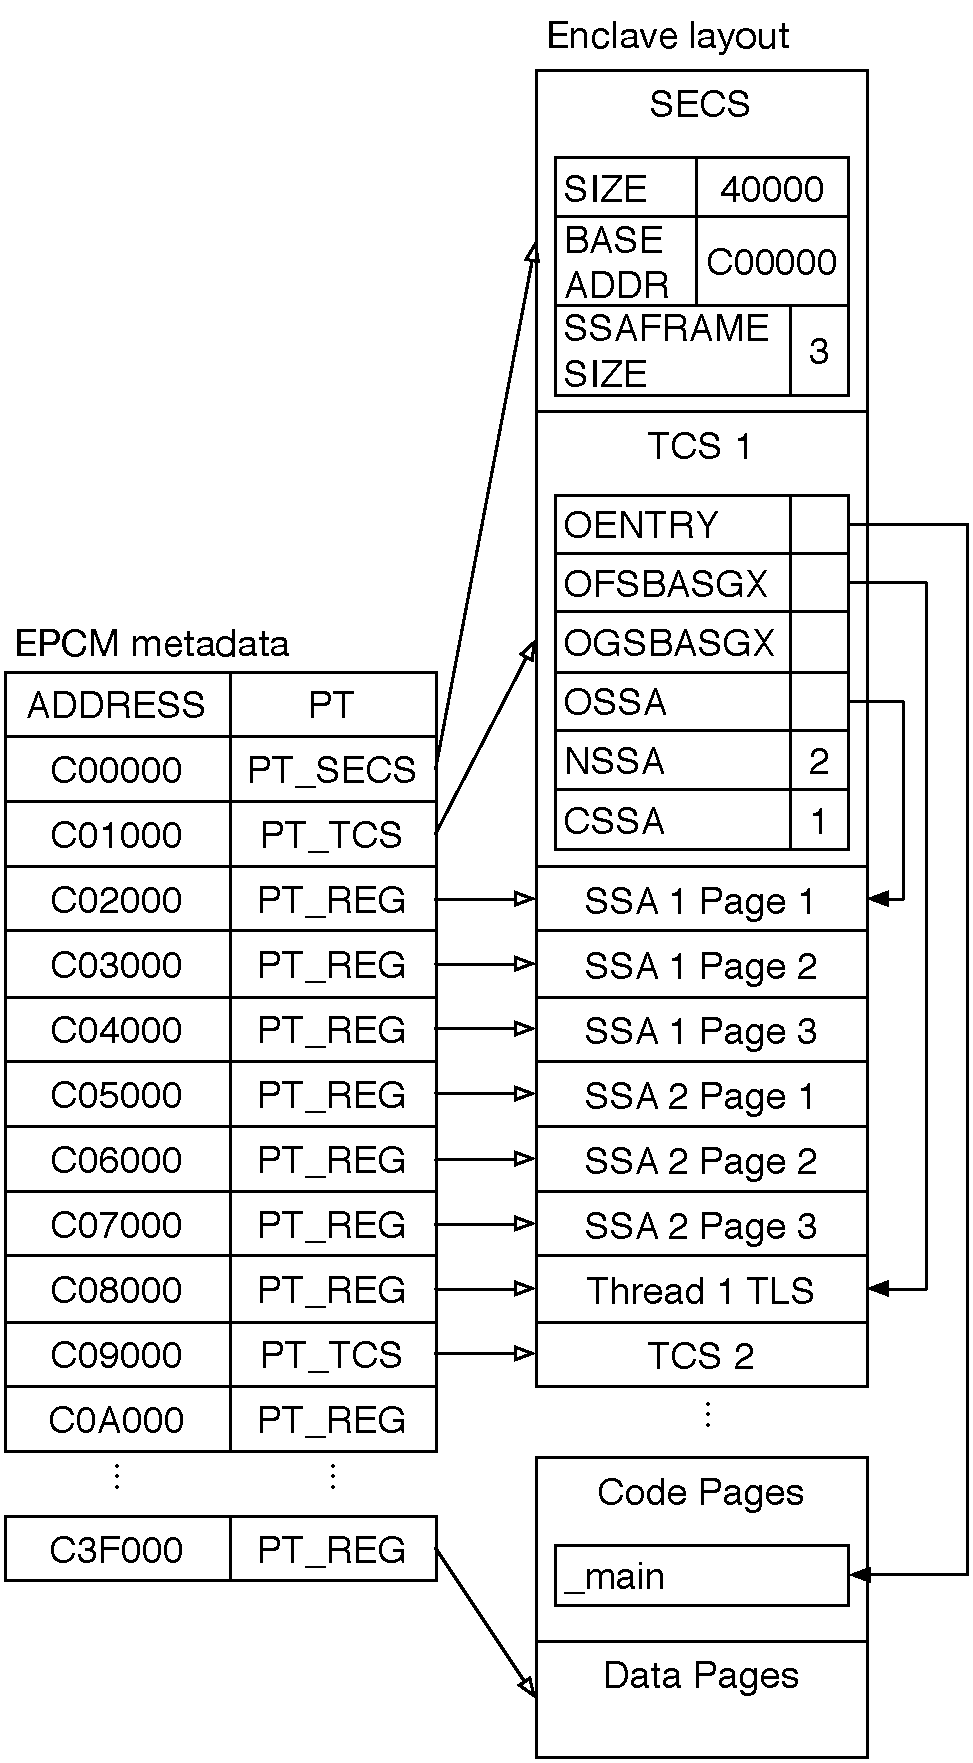
\includegraphics[width=70mm]{figures/enclave_layout.pdf}
  \caption{
    An enclave's memory layout. Each enclave has a SECS, and one TCS per
    supported hardware thread. Each TCS points to a sequence of SSAs, and
    specifies initial values for RIP, FS and GS.
  }
  \label{fig:enclave_layout}
\end{figure}

\subsubsection{The SGX Enclave Control Structure (SECS)}
\label{sec:secs}

% Data Structures and Enclave Operation: SDM S 37.4
% SGX Enclave Control Structure (SECS): SDM S 38.7, S 38.7.1
% Constructing an Enclave: SDM S 39.1
% ECREATE: SDM S 39.1.1, S 41.3
% Implicit vs. Explicit accesses: SDM S 38.5.3
% Implicit accesses: SDM S 38.5.3.2

The first step in creating an enclave is using the \texttt{ECREATE} instruction
to designate a previously unused EPC page as the enclave's \textit{SGX Enclave
Control Structure} (SECS). All instructions that operate on an enclave access
its control structure directly or indirectly.

% Internal CREGs: SDM S 41.1.4
% ECREATE: SDM S 39.1.1, S 41.3
% EWB: SDM S 41.3

The most important field in the SECS is the 64-bit \textit{enclave ID} (EID),
which is assigned by \texttt{ECREATE}. The EID identifies an enclave's pages in
the EPCM, so it must be unique across all the computer's active enclaves.
According to the ECREATE pseudo-code in the SDM, enclave IDs are allocated
using an atomic counter. An enclave's EID is generally hidden, as most SGX
instructions use the address of the enclave's SECS page as the enclave's
handler. However, the system software can learn an enclave's EID by evicting
one of its EPC pages (\S~\ref{sec:sgx_ewb}).

The software-visible SECS layout specifies the range of virtual addresses that
can be mapped to the enclave's EPC pages. Intel documentation calls the range
\textit{enclave linear address range} (ELRANGE). The range is specified using a
base (the BASEADDR field) and a size (the SIZE) field. ELRANGE must meet the
same constraints as a variable memory type range
(\S~\ref{sec:cacheability_config}), namely the size must be a power of 2, and
the base must be aligned to the size.

Currently, the main implication of ELRANGE is that all the SGX data structures
are initialized with enclave virtual addresses specified relatively to
BASEADDR. Furthermore, BASEADDR is not a part of the enclave's measurement
hash (details in \S~\ref{sec:measurement}). It follows that system software can
relocate an enclave in its host application's virtual address space, without
impacting the enclave's measurement hash.

Having ELRANGE follow the memory type range constraints provides a cheap way to
verify if a virtual address belongs to the address, in hardware. This provides
SGX engineers the option to implement per-enclave page tables in future SGX
revisions.

% Interactions with the Processor Extended State and Misc State: SDM S 42.7
% SECS.ATTRIBUTES.XFRM: SDM S 42.7.2.1

The software-visible SECS has an ATTRIBUTE field that specifies the Intel
achitecture features used by the enclave code. For example, the MODE64BIT flag
is set if the enclave targets the 64-bit Intel architecture, and the XFRM
sub-field contains the XCR0 register value expected by the enclave's code. XCR0
controls Intel architecture extensions such as SSE and AVX (see
\S~\ref{sec:registers}).

When a logical processor executes code inside an enclave, it sets XCR0 to the
value specified by the enclave's SECS, so malicious system software cannot
enable features that the enclave code is not prepared to handle. This lets
Intel introduce extensions that change the architectural behavior of existing
instructions, such as Memory Protection Extensions (MPX), without having to
worry about introducing security vulnerabilities in SGX enclaves written before
MPX.

The other fields in the software-visible SECS layout are used by the
software attestation process, which is explained in \S~\ref{sec:attestation}.


\subsubsection{The Thread Control Structure (TCS)}
\label{sec:tcs}

% Thread Control Structure (TCS): SDM S 38.8, S 38.8.{1,2,3,4}

A logical processor uses a \textit{Thread Control Structure} (TCS) while
executing code inside an enclave, so enclave authors must provision at least as
many TCS instances as the number of concurrent software threads that they want
to use.

The fields in the software-visible TCS layout direct the context switches
performed by a logical processor when it transitions between non-enclave and
enclave code.

% State Save Area (SSA): SDM S 38.9

In some cases (e.g., when receiving an interrupt), the processor needs to
preempt the execution of enclave code and start running kernel code. This is
accomplished by saving the enclave's context (register values) to an area
inside the enclave, called a \textit{State Save Area} (SSA).

Each TCS references a contiguous sequence of SSAs -- the OSSA field points to
the first SSA, and the NSSA field indicates the sequence's length. When a
logical processor needs to preempt enclave code, it uses the next available
SSA, indicated by the CSSA field in the TCS. The CPU refuses to execute enclave
code using a TCS where no SSA is available (CSSA $\ge$ NSSA).

An SSA essentially consists of the values of the general-purpose registers
(GPRs), and the result of running XSAVE (\S~\ref{sec:registers}) using the
feature mask specified in the ATTRIBUTES.XFRM field in the enclave's SECS.

% SECS.SSAFRAMESIZE: SDM S 42.7.2.2

Each SSA starts at the beginning of an EPC page, and takes up a fixed number of
EPC pages, specified in the SSAFRAMESIZE field in the enclave's SECS. The SSA
alignment and size restrictions most likely exist to simplify the SGX
implementation.

The TCS is stored in a page whose EPCM entry has the type PT\_TCS, and
therefore cannot be directly accessed by enclave software. However, SSAs are
stored in regular pages, so they are accessible to enclave software, and their
layout is defined in the SGX documentation.

\subsubsection{The Version Array (VA)}
\label{sec:va}

SGX includes support for system software to evict any EPC page to non-EPC RAM,
making it possible to have enclaves whose memory requirements exceed the
computer's EPC size. This is similar to ``swapping'', where the kernel evicts
pages of RAM to a hard disk while they are not accessed.

% Version Array (VA): SDM S 38.18
% EPC and Management of EPC Pages: SDM S 39.5, 39.5.{2,3,4,5,6}

The EWB instruction evicts an EPC page to non-EPC memory. In the process, it
creates an 8-byte nonce (called \textit{page version} in the Intel
documentation), which must be stored in an unused slot of a \textit{Version
Array} (VA). Evicted pages are brought back into the EPC by the ELDU and ELDB
instructions, which use the nonce produced by EWB, and clear the VA slot that
held the nonce.

System software uses the EPA instructions to mark an unused EPC page as a VA.
Pages that store VAs have the PT\_VA EPCM type, so the nonces generated by EWB
cannot be read, even by enclave software.  A VA page has 512 8-byte slots.
Unused slots are marked by the value 0 (zero), and EPA zeroes out the EPC page
used to store the VA.

Non-EPC memory can be accessed by system software, which is untrusted in the
SGX threat model, so EWB (illustrated in Figure~\ref{fig:sgx_ewb}) encrypts and
MACs the contents of the EPC page before storing it in untrusted memory. The
nonces stored in VA pages prevent replay attacks where malicious system
software would attempt to bring back an old version of an evicted EPC page.


\subsection {The Implementation of EPC Protection}

The memory controller is
integrated on the CPU die (see Figure~\ref{fig:cpu_die}), so it can be trusted
to prevent devices attached to the system bus from performing DMA transfers
to/from the PRM.

System software manages physical memory by directly modifying the contents of
page tables and EPTs (\S~\ref{sec:paging}), and is responsible for performing
TLB shootdowns (\S~\ref{sec:tlbs}) to ensure that the state not covered by
cache coherence \S~\ref{sec:cache_coherence} is synchronized across logical
processors. If the system software does not perform TLB shootdowns correctly,
application software can experience inconsistent views of memory.

In the context of SGX, an incorrect TLB shootdown can can result in having an
EPC page simultaneously accessible by two different enclaves, which would
compromise the SGX security guarantees. Therefore, the SGX instructions used
for EPC management ensure that the system software performs TLB shootdowns for
the entries that represent EPC pages.


% PRMRR documented in HASP papers and both SGX manuals, completely removed from
% SDM. It still exists in Coreboot. Couldn't find other Skywell code.
The SGX manual states that the EPC (the memory used to store enclave data) can
only be set up as UC or WB. While no further explanation is provided, we assume
that the UC option was provided in order to attempt to mitigate against some
cache-timing attacks.


\section{Enclave Operation}

SGX provides trusted computing by protecting the privacy and integrity of the
computation that is performed inside an enclave, and by providing remote
attestation identifying the software running inside an enclavee. This section
describes the processes used to set up an enclave and perform computation
inside it.

% TODO: find a place for the rest of this section
% Access Control Requirements: SDM S 38.3

Enclave code runs at ring 3 (\S~\ref{sec:rings}), just like application code,
so that it cannot interfere with the system software that manages resources.

% Interactions with VMX: SDM S 42.5, S 42.5.{1,2,3,4,5}

On most computers, the system software that manages SGX resources is an
operating system kernel. When VMX is in use, the hypervisor is responsible for
multiplexing SGX resources across the guest operating systems running in
virtual machines.



\section{Security Model}
\label{sec:attestation}

THe central context of SGX is the \textit{enclave}, a protected environment
that contains the code and data pertaining to a security-sensitive computation.
An SGX-enabled processor protects the integrity and privacy of the computation
inside an enclave by isolating the enclave's code and data from the outside
environment, including the operating system and hypervisor, and hardware
devices attached to the system bus. At the same time, the SGX model remains
compatible with the the traditional software layering in the Intel
architecture, where the OS kernel and hypervisor manage the computer's
resources. The rest of this section describes the security properties of
enclaves, discussing the trade-offs made while trying to balance security with
backwards compatibility.



Enclaves were designed to contain and protect the privacy-sensitive parts of an
application. All the code that handles private data must receive integrity
protection. Otherwise, a hostile environment could modify the code to leak
information about private data. Therefore, the SGX programming model prescribes
that code which accesses private data must be entirely contained inside an
enclave. Jumping into and out of enclave code must be performed explicitly
using the dedicated instructions \texttt{EENTER} and \texttt{EEXIT}.

The code inside an enclave runs at ring 3 (user mode), so it has the same
privileges as regular application code (see Figure \ref{fig:cpu_rings}).

\begin{figure}[hbtp]
  \center{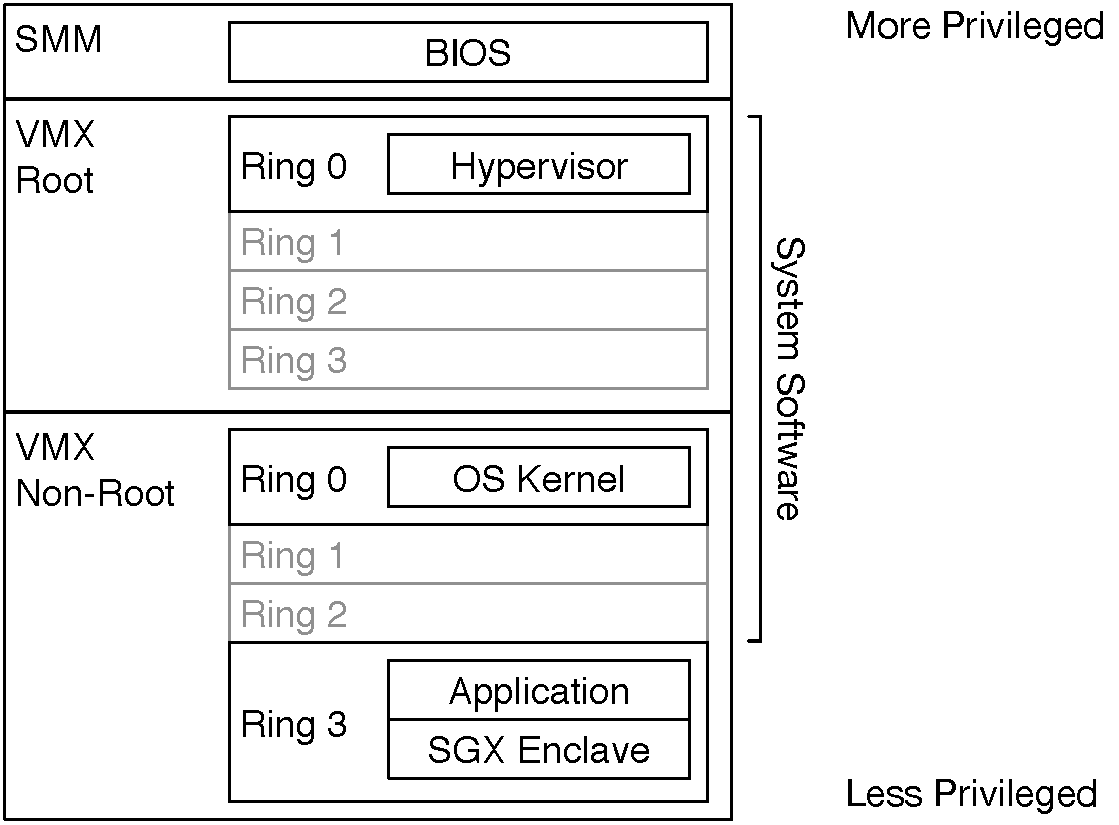
\includegraphics[width=75mm]{figures/cpu_rings.pdf}}
  \caption{
    Enclaves hold an application's private data and the code that operates on
    it. Therefore, they run at ring 3, in user mode.
  }
  \label{fig:computing_model}
\end{figure}

\HeadingLevelB{SGX Security Properties}
\label{sec:sgx_security_analysis}

We have summarized SGX's programming model and the implementation details
that are publicly documented in Intel's official documentation and published
patents. We are now ready to bring this the information together in an analysis
of SGX's security properties. We start the analysis by restating SGX's
security guarantees, and spend the bulk of this section discussing how SGX
fares when pitted against the attacks described in
\S~\ref{sec:security_background}.


\HeadingLevelC{Overview}

Intel's Software Guard Extensions (SGX) is Intel's latest iteration of a
trusted hardware solution to the secure remote computation problem. The SGX
design is centered around the ability to create an isolated container whose
contents receives special hardware protections that are intended to translate
into privacy, integrity, and freshness guarantees.

% ISCA 2015 SGX: Slide 93

An enclave's initial contents is loaded by the system software on the computer,
and therefore cannot contain secrets in plain text. Once initialized, an
enclave is expected to participate in a software attestation process, where it
authenticates itself to a remote server. Upon successful authentication, the
remote server is expected to disclose some secrets to an enclave over a
secure communication channel. The SGX design attempts to guarantee that the
measurement presented during software attestation accurately represents the
contents loaded into the enclave.

SGX also offers a certificate-based identity system that can be used to migrate
secrets between enclaves that have certificates issued by the same authority.
The migration process involves securing the secrets via authenticated
encryption before handing them off to the untrusted system software, which
passes them to another enclave that can decrypt them.

The same mechanism used for secret migration can also be used to cache the
secrets obtained via software attestation in an untrusted storage medium
managed by system software. This caching can reduce the number of times that
the software attestation process needs to be performed in a distributed system.
In fact, SGX's software attestation process is implemented by enclaves with
special privileges that use the certificate-based identity system to securely
store the CPU's attestation key in untrusted memory.


\HeadingLevelC{Physical Attacks}
\label{sec:sgx_vs_physical_attacks}

We begin by discussing SGX's resilience to the physical attacks described in
\S~\ref{sec:physical_attacks}. Unfortunately, this section is set to disappoint
readers expecting definitive statements. The lack of publicly available details
around the hardware implementation aspects of SGX precludes any rigorous
analysis. However, we do know enough about SGX's implementation to point out a
few avenues for future exploration.

Due to insufficient documentation, one can only hope that the SGX security
model is not trivially circumvented by a port
attack~(\S~\ref{sec:physical_port_attacks}). We are particularly concerned
about the Generic Debug eXternal
Connection~(GDXC)~\cite{yuffe2011sandybridge, intel2011gdxc}, which collects
and filters the data transferred by the uncore's ring bus
(\S~\ref{sec:cache_coherence}), and reports it to an external debugger.

The SGX memory protection measures are implemented at the core level, in the
Page Miss Handler~(PMH,~\S~\ref{sec:tlbs}) (\S~\ref{sec:sgx_access_protection})
and at the chip die level, in the memory controller
(\S~\ref{sec:sgx_uncore_modifications}). Therefore, the code and data inside
enclaves is stored in plaintext in on-chip caches~(\S~\ref{sec:caching}), which
entails that the enclave contents travels without any cryptographic protection
on the uncore's ring bus (\S~\ref{sec:cache_coherence}).

Fortunately, a recent Intel patent~\cite{shanbhogue2015gdxcsgx} indicates that
Intel engineers are tackling at least some classes of attacks targeting
debugging ports.

The SDM and SGX papers discuss the most obvious class of bus tapping
attacks~(\S~\ref{sec:physical_bus_attacks}), which is the DRAM bus tapping
attack. SGX's threat model considers DRAM and the bus connecting it to the CPU
chip to be untrusted. Therefore, SGX's Memory Encryption
Engine~(MEE,~\S~\ref{sec:sgx_uncore_modifications}) provides privacy, integrity
and freshness guarantees to the Enclave Page Cache~(EPC,~\S~\ref{sec:sgx_epc})
data while it is stored in DRAM.

However, both the SGX papers and the ISCA 2015 tutorial on SGX admit that the
MEE does not protect the addresses of the DRAM locations accessed when cache
lines holding EPC data are evicted or loaded. This provides an opportunity for
a malicious computer owner to observe an enclave's memory access patterns by
combining a DRAM address line bus tap with carefully crafted system software
that creates artificial pressure on the last-level
cache~(LLC~,\S~\ref{sec:caching}) lines that hold the enclave's EPC pages.

On a brighter note, as mentioned in \S~\ref{sec:physical_bus_attacks}, we are
not aware of any successful DRAM address line bus tapping attack. Furthermore,
SGX is vulnerable to cache timing attacks that can be carried out completely in
software, so malicious computer owners do not need to bother setting up a
physical attack to obtain an enclave's memory access patterns.

While the SGX documentation addresses DRAM bus tapping attacks, it makes no
mention of the System Management bus~(SMBus,~\S~\ref{sec:intel_me}) that
connects the Intel Management Engine~(ME,~\S~\ref{sec:intel_me}) to various
components on the computer's motherboard.

In \S~\ref{sec:sgx_vs_device_attacks}, we will explain that the ME might play a
role in SGX's software attestation process. This makes us concerned about the
possibility of an attack that taps the SMBus to reach into the Intel ME. The
SMBus is much more accessible than the DRAM bus, as it has fewer wires that
operate at a significantly lower speed. Unfortunately, without more information
about the role that the Intel ME plays in a computer, we cannot move beyond
speculation on this topic.

The threat model stated by the SGX design excludes physical attacks targeting
the CPU chip~(\S~\ref{sec:physical_chip_attacks}). Fortunately, Intel's patents
disclose an array of countermeasures aimed at increasing the cost of chip
attacks.

For example, the original SGX patents~\cite{intel2013patent1, intel2013patent2}
disclose that the Fused Seal Key and the Provisioning Key, which are stored in
e-fuses (\S~\ref{sec:sgx_quoting_enclave}), are encrypted with a \textit{global
wrapping logic key}~(GWK). The GWK is a 128-bit AES key that is hard-coded in
the processor's circuitry, and serves to increase the cost of extracting the
keys from an SGX-enabled processor.

As explained in \S~\ref{sec:physical_chip_attacks}, e-fuses have a large
feature size, which makes them relatively easy to ``read'' using a
high-resolution microscope. In comparison, the circuitry on the latest Intel
processors has a significantly smaller feature size, and is more difficult to
reverse engineer. Unfortunately, the GWK is shared among all the chip dies
created from the same mask, so it has all the drawbacks of global secrets
explained in \S~\ref{sec:physical_chip_attacks}.

Newer Intel patents~\cite{gotze2014provisioning, gotze2014provisioning2}
describe SGX-enabled processors that employ a \textit{Physical Unclonable
Function}~(PUF), e.g., \cite{suh2007puf}, \cite{maes2009puf}, which generates a
symmetric key that is used during the provisioning process.

Specifically, at an early provisioning stage, the PUF key is encrypted with the
GWK and transmitted to the key generation server. At a later stage, the key
generation server encrypts the key material that will be burned into the
processor chip's e-fuses with the PUF key, and transmits the encrypted material
to the chip. The PUF key increases the cost of obtaining a chip's fuse key
material, as an attacker must compromise both provisioning stages in order to
be able to decrypt the fuse key material.

As mentioned in previous sections, patents reveal design possibilities
considered by the SGX engineers. However, due to the length of timelines involved
in patent applications, patents necessarily describe earlier versions of the
SGX implementation plans, which might not match the shipping implementation. We
expect this might be the case with the PUF provisioning patents, as it makes
little sense to include a PUF in a chip die and rely on e-fuses and a GWK to
store SGX's root keys. Deriving the root keys from the PUF would be more
resilient to chip imaging attacks.

SGX's threat model excludes power analysis
attacks~(\S~\ref{sec:power_analysis_attacks}) and other side-channel attacks.
This is understandable, as power attacks cannot be addressed at the
architectural level. Defending against power attacks requires expensive
countermeasures at the lowest levels of hardware implementation, which can only
be designed by engineers who have deep expertise in both system security and
Intel's manufacturing process. It follows that defending against power analysis
attacks has a very high cost-to-benefit ratio.


\HeadingLevelC{Privileged Software Attacks}
\label{sec:sgx_vs_privileged_sw_attacks}

The SGX threat model considers system software to be untrusted. This is a
prerequisite for SGX to qualify as a solution to the secure remote computation
problem encountered by software developers who wish to take advantage of
Infrastructure-as-a-Service (IaaS) cloud computing.

SGX's approach is also an acknowledgement of the realities of today's software
landscape, where the system software that runs at high privilege
levels~(\S~\ref{sec:rings}) is so complex that security researchers constantly
find vulnerabilities in it (\S~\ref{sec:system_software_attacks}).

The SGX design prevents malicious software from directly reading or from
modifying the EPC pages that store an enclave's code and data. This security
property relies on two pillars in the SGX design.

First, the SGX implementation~(\S~\ref{sec:sgx_implementation_overview}) runs
in the processor's microcode~(\S~\ref{sec:microcode}), which is effectively a
higher privilege level that system software does not have access to.
Along the same lines, SGX's security
checks~(\S~\ref{sec:sgx_access_protection}) are the last step performed by the
PMH, so they cannot be bypassed by any other architectural feature.

This implementation detail is only briefly mentioned in SGX's official
documentation, but has a large impact on security. For context, Intel's Trusted
Execution Technology~(TXT,~\cite{grawrock2009txt}), which is the predecessor of
SGX, relied on Intel's Virtual Machine Extensions (VMX) for isolation. The
approach was unsound, because software running in System Management
Mode~(SMM,~\S~\ref{sec:rings}) could bypass the restrictions used by VMX to
provide isolation.

The security properties of SGX's memory protection mechanisms are discussed
in detail in \S~\ref{sec:sgx_vs_memory_mapping_attacks}.

Second, SGX's microcode is always involved when a CPU transitions between
enclave code and non-enclave code~(\S~\ref{sec:sgx_threads}), and therefore
regulates all interactions between system software and an enclave's
environment.

On enclave entry~(\S~\ref{sec:sgx_eenter}), the SGX implementation sets up the
registers~(\S~\ref{sec:resources}) that make up the execution
state~(\S~\ref{sec:registers}) of the logical
processor~(LP~\S~\ref{sec:cpu_core}), so a malicious OS or hypervisor cannot
induce faults in the enclave's software by tampering with its execution
environment.

When an LP transitions away from an enclave's code due to a
hardware exception~(\S~\ref{sec:faults}), the SGX implementation stashes the
LP's execution state into a State Save Area~(SSA,~\S~\ref{sec:sgx_ssa}) area
inside the enclave and scrubs it, so the system software's exception handler
cannot access any enclave secrets that may be stored in the execution state.

The protections described above apply to the all the levels of privileged
software. SGX's transitions between an enclave's code and non-enclave code
place SMM software on the same footing as the system software at lower
privilege levels. System Management Interrupts~(SMI,~\S~\ref{sec:interrupts},
\S~\ref{sec:system_software_attacks}), which cause the processor to execute
SMM code, are handled using the same Asynchronous Enclave
Exit~(AEX,~\S~\ref{sec:sgx_aex}) process as all other hardware exceptions.

Unfortunately, the following sections will reveal that while SGX offers rather
thorough against straightforward attacks on enclaves, its guarantees are almost
non-existent when it comes to more sophisticated attacks, such as side-channel
attacks. This section concludes by describing what might be the most egregious
side-channel vulnerability in SGX.

Most modern Intel processors feature hyper-threading. On these CPUs, the
execution units~(\S~\ref{sec:out_of_order}) and caches~(\S~\ref{sec:caching})
on a core~(\S~\ref{sec:cpu_core}) are shared by two LPs, each of which has its
own execution state. SGX does not prevent hyper-threading, so malicious system
software can schedule a thread executing the code of a victim enclave on an
LP that shares the core with an LP executing a snooping thread. This snooping
thread can use the processor's high-resolution performance counter
\cite{petters1999making}, in conjunction with microarchitectural knowledge of
the CPU's execution units and out-of-order scheduler, to learn the instructions
executed by the victim enclave, as well as its memory access patterns.

This vulnerability can be fixed using two approaches. The straightforward
solution is to require cloud computing providers to disable hyper-threading
when offering SGX. The SGX enclave measurement would have to be extended to
include the computer's hyper-threading configuration, so the remote parties in
the software attestation process can be assured that their enclaves are hosted
by a secure environment.

A more complex approach to fixing the hyper-threading vulnerability would
entail having the SGX implementation guarantee that when an LP is executing an
enclave's code, the other LP sharing its core is either inactive, or is
executing the same enclave's code. While this approach is possible, its design
would likely be quite cumbersome.


\HeadingLevelC{Memory Mapping Attacks}
\label{sec:sgx_vs_memory_mapping_attacks}

\S~\ref{sec:sgx_threads} explained that the code running inside an enclave uses
the same address translation process~(\S~\ref{sec:paging}) and page tables as
its host application. While this design approach makes it easy to retrofit SGX
support into existing codebases, it also enables the address translation
attacks described in \S~\ref{sec:address_translation_attacks}.

The SGX design protects the code inside enclaves against the active attacks
described in \S~\ref{sec:address_translation_attacks}. These protections have
been extensively discussed in prior sections, so we limit ourselves to
pointing out SGX's answer to each active attack. We also explain the lack of
protections against passive attacks, which can be used to learn an enclave's
memory access pattern at 4KB page granularity.

SGX uses the Enclave Page Cache Map~(EPCM,~\S~\ref{sec:sgx_epcm}) to store each
EPC page's position in its enclave's virtual address space. The EPCM is
consulted by SGX's extensions to the Page Miss
Handler~(PMH,~\S~\ref{sec:sgx_access_concepts}), which prevent straightforward
active address translation attacks~(\S~\ref{sec:memory_mapping_attacks}) by
rejecting undesirable address translations before they reach the
TLB~(\S~\ref{sec:tlbs}).

SGX allows system software to evict~(\S~\ref{sec:sgx_epc_eviction}) EPC pages
into untrusted DRAM, so that the EPC can be over-subscribed. The contents of
the evicted pages and the associated EPCM metadata are protected by
cryptographic primitives that offer privacy, integrity and freshness
guarantees. This protects against the active attacks using page swapping
described in \S~\ref{sec:page_swapping_attacks}.

When system software wishes to evict EPC pages, it must follow the process
described in \S~\ref{sec:sgx_eblock}, which guarantees to the SGX
implementation that all the LPs have invalidated any TLB entry associated with
pages that will be evicted. This defeats the active attacks based on stale TLB
entries described in \S~\ref{sec:tlb_mapping_attacks}.

\S~\ref{sec:sgx_access_correctness} outlines a correctness proof for all the
protection measures described above.

Unfortunately, SGX does not protect against passive address translation
attacks~(\S~\ref{sec:fault_tracking_attacks}), which can be used to learn an
enclave's memory access pattern at page granularity. While this appears
benign, recent work \cite{xu2015pagefaults} demonstrates the use of these
passive attacks in a few practical settings, which are immediately concerning
for image processing applications.

The rest of this section describes the theory behind planning a passive attack
against an SGX enclave. The reader is directed to \cite{xu2015pagefaults} for
a fully working system.

Passive address translation attacks rely on the fact that memory accesses
issued by SGX enclaves go through the Intel architecture's address translation
process~(\S~\ref{sec:paging}), including delivering page
faults~(\S~\ref{sec:faults}) and setting the accessed (A) and dirty (D)
attributes~(\S~\ref{sec:page_table_attributes}) on page table entries.

A malicious OS kernel or hypervisor can obtain the page-level trace of an
application executing inside an enclave by setting the present (P) attribute to
0 on all the enclave's pages before starting enclave execution. While an
enclave executes, the malicious system software maintains exactly one
instruction page and one data page present in the enclave's address space.

When a page fault is generated, CR2 contains the virtual address of a page
accessed by enclave, and the error code indicates whether the memory access was
a read or a write (bit 1) and whether the memory access is a data access or
an instruction fetch access (bit 4). On a data access, the kernel tracing the
enclave code's memory access pattern would set the P flag of the desired page
to 1, and set the P flag of the previously accessed data page to 0. Instruction
accesses can be handled in a similar manner.

For a slightly more detailed trace, the kernel can set a desired page's
writable (W) attribute to 0 if the page fault's error code indicates a read
access, and only set it to 1 for write accesses. Also, applications that use a
page as both code and data (self-modifying code and just-in-time compiling VMs)
can be handled by setting a page's disable execution (XD) flag to 0 for a data
access, and by carefully accounting for the case where the last accessed data
page is the same as the last accessed code page.

Leaving an enclave via an Asynchronous Enclave Exit~(AEX,~\S~\ref{sec:sgx_aex})
and re-entering the enclave via \texttt{ERESUME}~(\S~\ref{sec:sgx_eresume})
causes the CPU to flush TLB entries that contain enclave addresses, so a
tracing kernel would not need to worry about flushing the TLB. The tracing
kernel does not need to flush the caches either, because the CPU needs to
perform address translation even for cached data.

A straightforward way to reduce this attack's power is to increase the page
size, so the trace contains less information. However, the attack cannot be
completely prevented without removing the kernel's ability to oversubscribe the
EPC, which is a major benefit of paging.


\HeadingLevelC{Software Attacks on Peripherals}
\label{sec:sgx_vs_device_attacks}

Since the SGX design does not trust the system software, it must be prepared to
withstand the attacks described in \S~\ref{sec:device_attacks}, which can be
carried out by the system software thanks to its ability to control peripheral
devices on the computer's motherboard~(\S~\ref{sec:motherboard}). This section
summarizes the security properties of SGX when faced with these attacks, based
on publicly available information.

When SGX is enabled on an LP, it configures the memory
controller~(MC,~\S~\ref{sec:cache_coherence}) integrated on the CPU chip die to
reject any DMA transfer that falls within the Processor Reserved
Memory~(PRM,~\S~\ref{sec:sgx_prm}) range. The PRM includes the EPC, so the
enclaves' contents is protected from the PCI Express attacks described in
\S~\ref{sec:pcie_attacks}. This protection guarantee relies on the fact that
the MC is integrated on the processor's chip die, so the MC configuration
commands issued by SGX's microcode
implementation~(\S~\ref{sec:sgx_microcode_modifications}) are transmitted over
a communication path that never leaves the CPU die, and therefore can be
trusted.

SGX regards DRAM as an untrusted storage medium, and uses cryptographic
primitives implemented in the MEE to guarantee the privacy, integrity and
freshness of the EPC contents that is stored into DRAM. This protects against
software attacks on DRAM's integrity, like the rowhammer attack described in
\S~\ref{sec:rowhammer_attack}.

% Interaction with Performance Monitoring: SDM S 43.6

The SDM describes an array of measures that SGX takes to disable processor
features intended for debugging when a LP starts executing an enclave's code.
For example, enclave entry~(\S~\ref{sec:sgx_eenter}) disables Precise Event
Based Sampling (PEBS) for the LP, as well as any hardware breakpoints placed
inside the enclave's virtual address range~(ELRANGE,~\S~\ref{sec:sgx_elrange}).
This addresses some of the attacks described in \S~\ref{sec:perfmon_attacks},
which take advantage of performance monitoring features to get information that
typically requires access to hardware probes.

% ISCA 2015 SGX Slide 115:
%   "Software Side-Channel Adversary"

At the same time, the SDM does not mention anything about uncore PEBS counters,
which can be used to learn about an enclave's LLC activity. Furthermore, the
ISCA 2015 tutorial slides mention that \textbf{SGX does not protect against
software side-channel attacks} that rely on performance counters.

This limitation in SGX's threat model leaves security-conscious enclave authors
in a rather terrible situation. These authors know that SGX does not protect
their enclaves against a class of software attacks. At the same time, they
cannot even contemplate attempting to defeat these attacks on their own, due to
lack of information. Specifically, the documentation that is publicly available
from Intel does not provide enough information to model the information leakage
due to performance counters.

For example, Intel does not document the mapping implemented in
CBoxes~(\S~\ref{sec:cache_coherence}) between physical DRAM addresses and the
LLC slices used to cache the addresses. This mapping impacts several uncore
performance counters, and the impact is strong enough to allow security
researches to reverse-engineer the mapping \cite{inci2015rsachannel,
maurice2015intelhash, yarom2015intelhash}. Therefore, it is safe to assume that
a malicious computer owner who knows the CBox mapping can use the uncore
performance counters to learn about an enclave's memory access patterns.

The SGX papers mention that SGX's threat model includes attacks that overwrite
the flash memory chip that stores the computer's firmware, which result in
malicious code running in SMM.  However, all the official SGX documentation is
silent about the implications of an attack that compromises the firmware
executed by the Intel ME.

\S~\ref{sec:firmware_attacks} states that the ME's firmware is stored in the
same flash memory as the boot firmware, and enumerates some of ME's special
privileges that enable it to help system administrators remotely diagnose and
fix hardware and software issues. Given that the SGX design is concerned about
the possibility of malicious computer firmware, it is reasonable to be
concerned about malicious ME firmware.

\S~\ref{sec:firmware_attacks} argues that an attacker who compromises the ME
can carry out actions that are usually classified as physical attacks.
Fortunately, the most scary attack vector afforded by an ME takeover appears to
be direct DRAM access, and SGX already assumes that the DRAM is untrusted.
Therefore, an ME compromise would be equivalent to the DRAM attacks analyzed in
\S~\ref{sec:sgx_vs_physical_attacks}.


\HeadingLevelC{Cache Timing Attacks}
\label{sec:sgx_vs_cache_timing_attacks}

The SGX threat model excludes the cache timing attacks described in
\S~\ref{sec:cache_timing}. The SGX documentation bundles these attacks together
with other side-channel attacks and summarily dismisses them as complex physical
attacks. However, cache timing attacks can be mounted entirely by unprivileged
software running at ring 3. This section describes the implications of SGX's
environment and threat model on cache timing attacks.

The main difference between SGX and a standard architecture is that SGX's
threat model considers the system software to be untrusted. As explained
earlier, this accurately captures the situation in remote computation
scenarios, such as cloud computing. SGX's threat model implies that the system
software can be carrying out a cache timing attack on the software inside an
enclave.

A malicious system software translates into significantly more powerful cache
timing attacks, compared to those described in \S~\ref{sec:cache_timing}. The
system software is in charge of scheduling threads on LPs, and also in charge
of setting up the page tables used by address
translation~(\S~\ref{sec:paging}), which control cache
placement~(\S~\ref{sec:tlbs}).

For example, the malicious kernel set out to trace an enclave's memory access
patterns described in \S~\ref{sec:sgx_vs_memory_mapping_attacks} can improve
the accuracy of a cache timing attack by using page
coloring~\cite{kessler1992coloring} principles to
partition~\cite{lin2008coloring} the cache targeted by the attack. In a
nutshell, the kernel divides the cache's sets~(\S~\ref{sec:cache_org}) into
two regions, as shown in Figure~\ref{fig:cache_partitions}.

\begin{figure}[hbt]
  \centering
  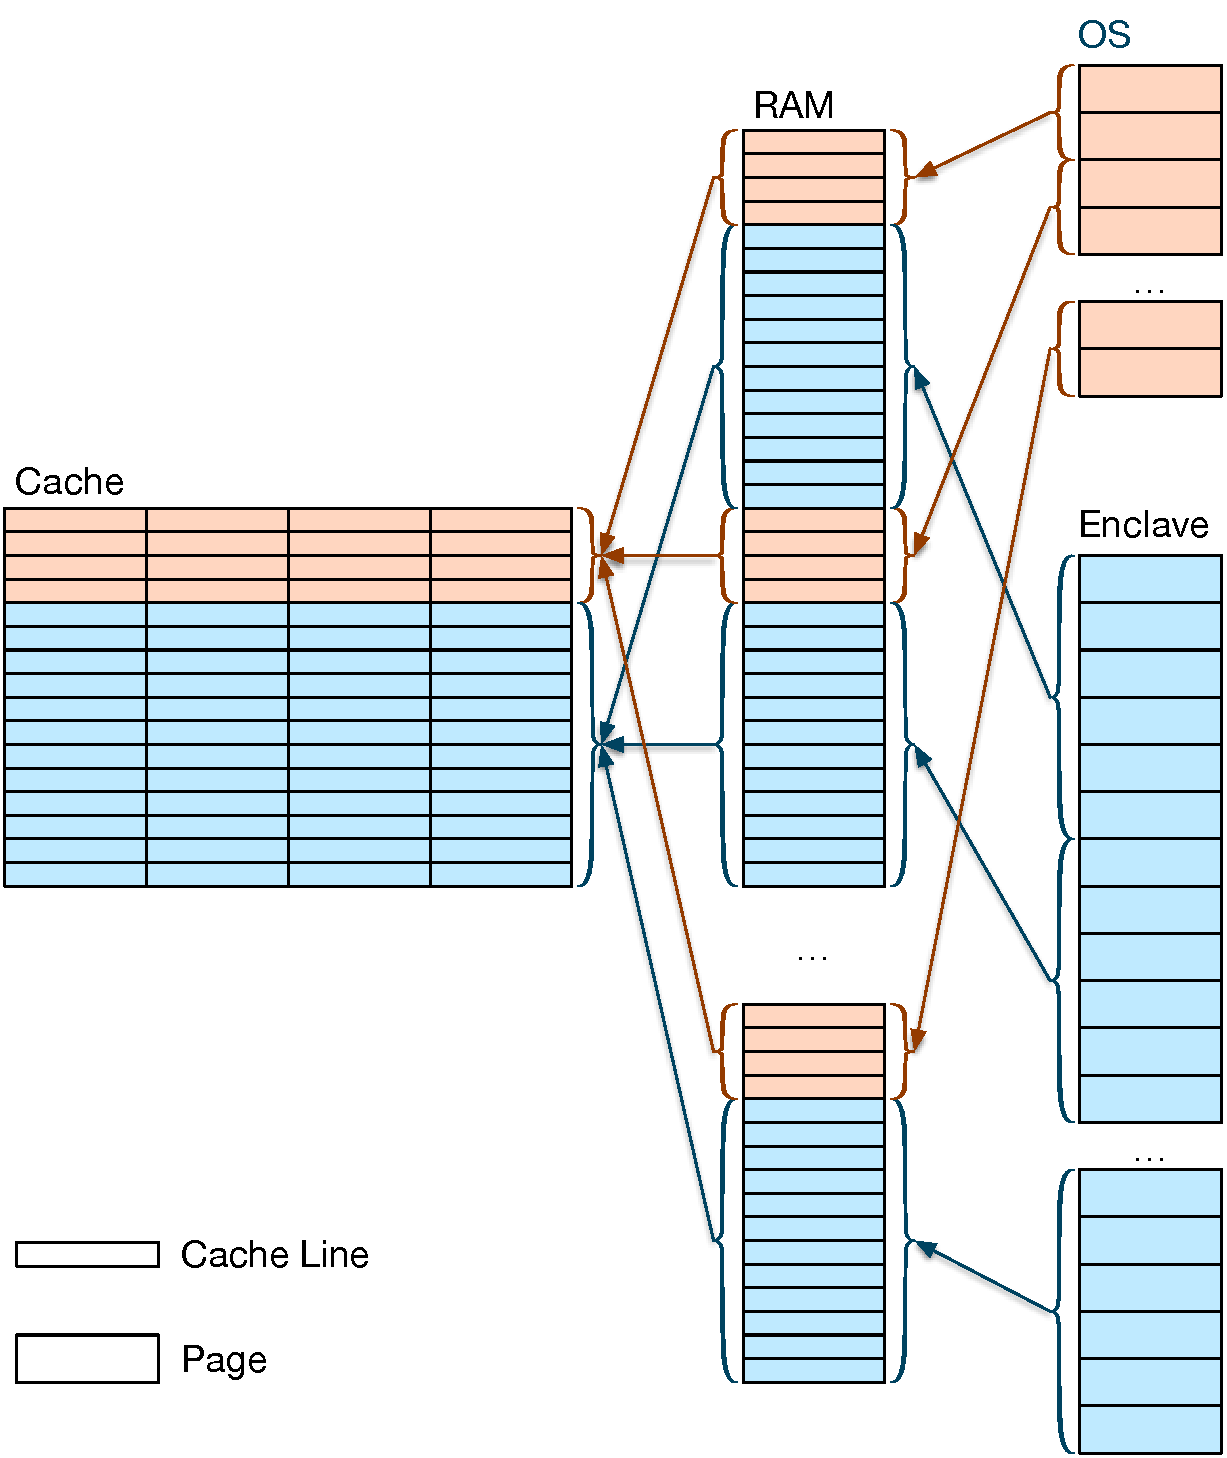
\includegraphics[width=85mm]{figures/cache_partitions.pdf}
  \caption{
    A malicious OS can partition a cache between the software running inside an
    enclave and its own malicious code. Both the OS and the enclave software
    have cache sets dedicated to them. When allocating DRAM to itself and to
    the enclave software, the malicious OS is careful to only use DRAM regions
    that map to the appropriate cache sets. On a system with an Intel CPU, the
    the OS can partition the L2 cache by manipulating the page tables in a way
    that is completely oblivious to the enclave's software.
  }
  \label{fig:cache_partitions}
\end{figure}

The system software stores all the victim enclave's code and data in DRAM
addresses that map to the cache sets in one of the regions, and stores its own
code and data in DRAM addresses that map to the other region's cache sets.  The
snooping thread's code is assumed to be a part of the OS. For example, in a
typical 256~KB (per-core) L2 cache organized as 512 8-way sets of 64-byte
lines, the tracing kernel could allocate lines 0-63 for the enclave's code
page, lines 64-127 for the enclave's data page, and use lines 128-511 for its
own pages.

To the best of our knowledge, there is no minor modification to SGX that would
provably defend against cache timing attacks. However, the SGX design could
take a few steps to increase the cost of cache timing attacks. For example,
SGX's enclave entry implementation could flush the core's private caches, which
would prevent cache timing attacks from targeting them. This measure would
defeat the cache timing attacks described below, and would only be vulnerable
to more sophisticated attacks that target the shared LLC, such as
\cite{yarom2013llctiming, liu2015llctiming}. The description above assumes that
multi-threading has been disabled, for the reasons explained in
\S~\ref{sec:sgx_vs_privileged_sw_attacks}.

Barring the additional protection measures described above, a tracing kernel
can extend the attack described in \S~\ref{sec:sgx_vs_memory_mapping_attacks}
with the steps outlined below to take advantage of cache timing and narrow down the
addresses in an application's memory access trace to cache line granularity.

Right before entering an enclave via \texttt{EENTER} or \texttt{ERESUME}, the
kernel would issue \texttt{CLFLUSH} instructions to flush the enclave's code
page and data page from the cache. The enclave could have accessed a single
code page and a single data page, so flushing the cache should be reasonably
efficient. The tracing kernel then uses 16 bogus pages (8 for the enclave's
code page, and 8 for the enclave's data page) to load all the 8 ways in the 128
cache sets allocated by enclave pages. After an AEX gives control back to the
tracing kernel, it can read the 16 bogus pages, and exploit the time difference
between an L2 cache hit and a miss to see which cache lines were evicted and
replaced by the enclave's memory accesses.

% PRMRR documented in HASP papers and both SGX manuals, completely removed from
% SDM. It still exists in Coreboot. Couldn't find other Skywell code.

An extreme approach that can provably defeat cache timing attacks is disabling
caching for the PRM range, which contains the EPC. The SDM is almost completely
silent about the PRM, but the SGX manuals that it is based on state that
the allowable caching behaviors~(\S~\ref{sec:cacheability_config}) for the EPC
are uncacheable (UC) and write-back (WB). This could become useful if the SGX
implementation would make sure that the PRM's caching behavior cannot be
changed while SGX is enabled, and if the selected behavior would be captured by
the enclave's measurement~(\S~\ref{sec:sgx_measurement}).

\section{The Hardware Underpinnings of SGX}

The security of SGX hinges on the assumption that it is very difficult for an
attacker to produce an attestation that contains attacker-supplied information
in the enclave field. In order to evaluate this claim, we must understand the
hardware protection mechanisms and the encryption schemes involved in the
process.

Most of the material in this section comes from Intel's
patents~\cite{intel2013patent1, intel2013patent2}, because the SGX papers and
reference consider this information an implementation detail. We point out when
a piece of information matches the SGX manual or one of the SGX papers.

According to the Intel patents, the SGX instructions are implemented in
microcode. The statement in \cite{anati2013sgx} that a microcode update changes
the platform TCB confirms this finding. The patents state that SGX requires
very few hardware changes, and most of the implementation is in microcode, as a
positive fact, fueling our suspicion that minimizing hardware changes was a
high priority in the SGX design.


\subsection{Memory Protection Mechanisms}

The SGX reference manual states that the Processor Reserved Memory (PRM) is
allocated by the BIOS, by setting the PRM range registers (PRMRR). The patents
refer to this range as the secure enclave range registers (SERR), and state
that the memory range is protected from DMA accesses by a dedicated pair of
SAD / TAD entries (\S~\ref{sec:cpu_uncore}).
The patents state that the SAD and TAD entries mirror the PRMRR registers
which, if done correctly, does prevent against DMA snooping.

The SGX reference manual states that the EPC memory is protected against
physical snooping attacks on the DRAM by an implementation-dependent mechanism,
and suggests that the most likely implementation is a Memory Encryption Engine
(MEE). The MEE is called a crypto engine in the Intel patents, which state that
the crypto engine is connected to the QuickPath Interconnect (QPI) home agent
in each processor, and it encrypts all RAM accesses in a range called the
Crypto Memory Aperture (CMA), before they reach the memory controller. The CMA
range is configured by setting the Crypto Memory Range Registers (CMRR). The
CMA contains the EPC, EPCM, and other data structured used by the SGX
implementations, which leads us to believe that the CMA covers the entire PRM
range, and the CMRR and PRMRR are identical. One of the SGX
papers~\cite{mckeen2013sgx} states that the PRM may be covered by one or more
MEE regions.

The data inside the CMA is lost when the CPU is powered down (including when it
enters the S3 power management state), so enclaves must be either torn down by
the OS, or their EPC pages must be evicted to RAM, and eventually to disk.

The EPC encryption described above is only intended to defend against physical
attacks. Enclaves are isolated from system software (the OS and hypervisor) by
access control checks in the CPU, as described in \S~\ref{sec:epcm}. The
patents specify the protection algorithm with more clarity.

The patents also specify that the memory access checks are performed in the
Page-Miss Handler (PMH) microcode, which is invoked during TLB misses. The PMH
performs the SGX access checks described below. If the access checks succeed,
the PMH creates a TLB entry, as it normally would. If the access checks fail,
the PMH aborts, which results in a Page Fault. The desire to restrict SGX
access checks to the PMH introduces the requirement to flush a logical
processor's TLBs when it enters or exits enclave mode. This is accomplished by
adding 1 bit to TLB entries, which differentiates between enclave pages and
non-enclave pages.
On enclave entry and exit, all the TLB entries that have the enclave bit set
are flushed. One of the SGX papers~\cite{mckeen2013sgx} confirms that the EPCM
is checked by the PMH.
The SGX manual also confirms this: ``The Intel SGX access control itself is
implemented as an extension to the traditional IA-32 paging/EPT state
machine.''
The Intel patents state that future implementations may optimize away the TLB
flushes by adding enclave ID tags to TLB entries.

The SGX access checks occur after the normal page address translation process
(described in the Intel SDM) completes.
If the resulting physical address does not fall within the CMA, the
SGX access checks do not apply.
A CMA memory access is only allowed if originates from the CPU's microcode
(used to implement the SGX instructions), or if it an admissible enclave
access.
The latter is true if the logical processor making the memory access is in
enclave mode, the accessed physical address falls in an EPC range, the page's
EPCM entry has the present (P) bit set and does not have the blocked (B) bit
set, the current enclave's ID matches the enclave ID in the page's EPCM entry,
and the linear address used to access the page matches the one in the page's
EPCM entry.

The Intel patents call ELRANGE the Enclave Linear Space (ELS) range.



\subsection{Key Hierarchy and Derivation}

According to Intel's patents, the SGX implementation relies on a complex key
derivation process rooted on global secret keys in the CPU circuitry, and on
secrets embedded in the processor's eFUSEs. eFUSE information can be extracted
efficiently (Chipworks quoted us \$50-250k for extracting the entire eFUSE
contents from an Intel i5 processor), so some of the eFUSE secrets are
encrypted with a master key (referred to as a ``global wrapping logic key'' in
the patents).

The patents state that encrypting the eFUSE secrets by the logic key makes them
harder to extract via hardware monitoring tools, and protects them while in
transit to the CPU during the manufacturing process. This assumes that it is
very expensive to obtain the global key from a CPU, by virtue of the low
feature size.

The SGX patents describe two ``logic keys'' embedded in the CPU's circuitry,
which are the same for all CPUs in a stepping, making them essentially global
keys. The \textit{global wrapping logic key} is a 128-bit AES key, and it is
used to encrypt a subset a 256-bit A.x value used to re-create the CPU's EPID
key, and a 128-bit \textit{pre-seed key 0}. The eFUSEs also contain a 128-bit
\textit{pre-seed key 1} and a 32-bit EPID group ID, which are stored in
cleartext.

The SGX manuals~\cite{intel2013sgxmanual, intel2014sgx2manual} mention a
16-byte CPU security version number (SVN), which contains the version numbers
of various TCB components, and is a source in the key derivation process. The
patents further specify that the SVN register is made up of (most likely 8-bit)
sections that contain the SVNs of each layer in the SGX initialization process,
and that each initialization step sets the corresponding section to its SVN,
and then locks it for the duration of the power-up cycle.

Intel's patents disclose that the key derivation process uses 128-bit AES in
ECB mode as a pseudo-random function (PRF). When an SVN is an input to a key
derivation process, a \textit{PRF loop} is used, where the PRF is applied to
a constant



\cite{anati2013sgx} confirms that the attestation uses Intel's
EPID~\cite{brickell2009epid} group signature scheme.


Key Request Inputs

\begin{table}[hbt]
  \center{\begin{tabularx}{\columnwidth}{| l | l | X |}
  \hline
  \textbf{Name} & \textbf{Size} & \textbf{Description}\\
  \hline
  Key Name & 2 & Which key will be derived \\
  \hline
  Policy & 2 & Whether the key derivation uses MRENCLAVE or MRSIGNER \\
  \hline
  ISV SVN & 2 & Developer-assigned SVN \\
  \hline
  CPU SVN & 16 & 128-bit TCB SVN \\
  \hline
  KeyID & 32 & Used for wear-out protection \\
  \hline
  Attribute Mask & 16 & Which SECS ATTRIBUTES are used in Seal Key \\
  \hline
  MISC Mask & 2 & Which SECS MISCSELECT bits are used in Seal Key \\
  \hline
  \end{tabularx}}
  \caption{Values of the PT (page type) field in an EPCM entry.}
  \label{fig:key_request_inputs}
\end{table}

Key names: LAUNCH, PROVISION, PROVISION\_SEAL, REPORT, SEAL.


\subsection{Data Structures}

The Intel patents state that the 128-bit enclave key is stored in the enclave's
SECS page, and that SGX security depends on enclaves not being able to read
their own SECS pages. They also state that the enclave key is used to encrypt
the EPC pages when they are evicted to untrusted RAM. The patents also state
that the enclave's SECS page contains the SVN of the launch permit creator.

The Intel patents state that each TCS has two fields that store the values of
the DR7 and IA32\_DEBUGCTL registers during EENTER, and are used to restore the
original values during EEXIT and AEX.

The Intel patents state that the enclave ID used in EPCM entries is the
phyisical address of the page holding the enclave's SECS, without the bottom
12 bits that are guaranteed to be zero. The SGX manual indicates that when an
EPC page is allocated via EADD, the physical address of its enclave's SECS is
cached, until the page is removed via EREMOVE. This, together with the fact
that the enclave ID's location in the SECS is not specified, indicates that the
enclave's ID is indeed the physical address of its SECS page.


The Intel patents indicate that EREPORT's KeyID is initialized to a random
value on each processor power cycle, and is incremented after $2^{32}$ AES
operations that use the value. They also indicate that each EREPORT may
increment the KeyID by 1.




\section{Software Guard Extensions (SGX)}
\label{sec:sgx}

This section summarizes the aspects of the SGX documentation that are relevant
to our system. The interested but time-constrained reader is advised to read
\cite{mckeen2013innovative}, \cite{anati2013sgx}, and Chapters 1 (Introduction
to SGX), 3 (Enclave Operation), 4 (Enclave Exiting Events) and 6 (SGX
Interactions with IA32 and Intel 64 Architecture) of \cite{intel2013sgxmanual}
for a deeper understanding of SGX.


\subsection{SGX Overview}
\label{sec:sgx_overview}

SGX introduces a protected execution environment, called an \textit{enclave}.
An enclave's code and data are protected by placing them inside the Enclave
Page Cache (EPC), which is a subset of the Processor Reserved Memory (PRM)
area. The EPC is split in 4KB pages. Each page is associated with an enclave.
EPC page memory accesses coming from code outside the EPC page's enclave are
blocked by the CPU. This access check covers all privilege levels, including
SMM. The memory controller inside the CPU blocks any DMA access to PRM, so EPC
pages cannot be accessed by hardware via DMA.

The EPC contents is encrypted\footnote{Actually, the SGX manual carefully
tiptoes around this issue by saying ``On implementations in which EPC is part
of system DRAM, the contents of the EPC are protected by an encryption
engine.''} as it leaves the CPU, to prevent against bus tapping attacks.
Although the data is encrypted, the memory addresses are not protected,
exposing the enclave code's memory access patterns.

Execution flow can only enter an enclave via special CPU instructions
(\texttt{EENTER}, \texttt{ERESUME}, \texttt{EEXIT}), which are similar to the
mechanism for switching from user mode to kernel mode. Enclave execution always
happens in protected mode, at ring 3, and uses the address translation set up
by the OS kernel and hypervisor (\S \ref{sec:paging}). \texttt{EENTER}
transfers control to a predefined entry point in the enclave, and
\texttt{EEXIT} leaves the enclave.

To avoid leaking private data, a CPU that is executing enclave code does not
directly service an interrupt, fault (e.g., a page fault) or VM exit. Instead,
the CPU first performs an Asynchronous Enclave Exit (AEX) to switch from
enclave code to ring 3 code, and then services the interrupt, fault, or VM
exit.  The CPU performs an AEX by saving the CPU state into a predefined area
inside the enclave and transfers control to a pre-specified instruction outside
the enclave, replacing CPU registers with synthetic values. After the
interrupt, fault or VM exit is serviced, its handler returns control to ring 3
code outside the enclave, which performs an \texttt{ERESUME}, which transfers
control back into the enclave and restores the CPU state at the time the
enclave execution was interrupted.

The allocation of EPC pages to enclaves is delegated to the OS kernel (or
hypervisor), and done via dedicated ring 0 CPU instructions. \texttt{EADD}
allocates new pages to an enclave under construction, and \texttt{EREMOVE}
deallocates pages during enclave tear-down. \texttt{EWB} evicts\footnote{
Multi-threaded enclaves require more steps that are orthogonal to the issues
addressed by this work.} an EPC page to RAM space that the OS kernel can
access, and \texttt{ELDB}\footnote{SGX specifies two related instructions,
\texttt{ELDB} and \texttt{ELDU}. The distinction is irrelevant for our
purposes.} loads a previously evicted page from kernel-acessible RAM back into
the EPC.

\texttt{EADD} associates each EPC page with a virtual address used to access
it, and the association is maintained by the \texttt{EWB} / \texttt{ELDB} pair.
The CPU enforces\footnote{The CPU generates a general protection fault (\#GP)
if an address translation that results in an EPC page uses the wrong virtual
address as input.} the invariant that an EPC page can only be accessed using
the virtual address associated with it. This mechanism ensures that the OS
kernel and hypervisor maintain a consistent mapping of virtual addresses to
EPC pages. The CPU encrypts and HMACs pages evicted with \texttt{EWB},
providing privacy and integrity guarantees, including protection against replay
attacks. The details are described in \cite{intel2013sgxmanual}.

Page faults in enclave code are handled using the AEX process. The CR2
register, which normally holds the virtual address that causes the fault, has
its bottom 12 bits set to zero. The other bits of CR2 are necessary for the OS
kernel or hypervisor to know which page needs to be loaded in RAM or into the
EPC. This allows a curious OS kernel or hypervisor to obtain a page-level
memory access trace for a program running inside an enclave, simply by making
sure that only one page is present at any given time.


\subsection{SGX Information Leaks}
\label{sec:sgx_leaks}

Software Guard Extensions, as documented in \cite{intel2013sgxmanual}, does not
provide full privacy guarantees to the code executing inside an enclave. We
present methods that an attacker can use to extract information from an
enclave.

\subsubsection{Hyper-Threading Leaks}

Modern Intel CPUs feature hyper-threading, which means that each core has two
(or more) sets of register files and local APICs, presented as logical
processors running separate threads (see Figure \ref{fig:cpu_core}). The
threads share the other core resources, such as the fetch and decode units,
execution units and L1 and L2 caches. SGX does not prevent hyper-threading, so
a malicious OS kernel or hypervisor can schedule a thread executing enclave
code and a snooping thread on logical processors on same core. The snooping
thread can use the processor's high-resolution performance counter
\cite{petters1999making} to get information about the instructions and memory
access patterns of the thread executing enclave code.

A promising approach for preventing against hyper-threading leaks is to
effectively disable hyper-threading, by using \texttt{CPUID} to find out the
number of logical processors in the current core, and to require the OS to
schedule threads in the same enclave on all the logical processors. This could
be implemented by having the main thread spinlock waiting for the other threads
to start, before any protected computation is performed. However, a malicious
kernel or hypervisor can de-schedule the other threads after the main thread
performed the spinlock check, so this defense is not reliable.

\subsubsection{Page-Level Memory Access Leaks}

While executing the code inside an enclave, the CPU still follows the standard
page translation process (\S \ref{sec:paging}), including setting the A and D
bits and delivering page faults. A malicious OS kernel or hypervisor can
obtain the page-level trace of an application executing inside an enclave by
setting the P flag to 0 on all the enclave's pages before starting enclave
execution, and then maintaining exactly one instruction page and one data page
present in the enclave's address space.

When a page fault is generated, CR2 contains the virtual address of a page
accessed by enclave, and the error code indicates whether the memory access was
a read or a write (bit 1) and whether the memory access is a data access or
an instruction fetch access (bit 4). On a data access, the kernel tracing the
enclave code's memory access pattern would set the P flag of the desired page
to 1, and set the P flag of the previously accessed data page to 0. Instruction
accesses can be handled in a similar manner.

For a slightly more detailed trace, the kernel can set a desired page's W flag
to 0 if the page fault's error code indicates a read access, and only set it to
1 for write accesses. Also, applications that use a page as both code and data
(self-modifying code and just-in-time compiling VMs) can be handled by setting
a page's XD flag to 0 for a data access, and by carefully accounting for the
case where the last accessed data page is the same as the last accessed code
page.

Leaving an enclave via an AEX and re-entering the enclave via \texttt{ERESUME}
causes the CPU to flush TLB entries that contain enclave addresses, so a
tracing kernel would not need to worry about flushing the TLB. The tracing
kernel does not need to flush the caches either, because the CPU needs to
perform address translation even for cached data.

An easy way to reduce this attack's power is to increase the page size, so the
trace contains less information. However, the attack cannot be completely
prevented without removing the kernel's ability to oversubscribe the EPC,
which is a major benefit of paging.

\subsubsection{Fine-Grained Memory Access Leaks}

The AEX process and the \texttt{ERESUME} instructions do not flush the CPU
caches. A tracing kernel can take advantage of cache timing to narrow down
the addresses in an application's memory access trace to cache line
granularity, by extending the method described above with the steps below.

The tracing kernel controls the mapping between virtual addresses and physical
addresses, so it can make sure that its own code and data use different sets
in the L2 cache from the enclave's code and data. For example, in a typical
256kb (per-core) L2 cache organized as 512 8-way sets of 64-byte lines, the
tracing kernel could allocate lines 0-63 for the enclave's code page, lines
64-127 for the enclave's data page, and use lines 128-511 for its own pages.

Right before entering an enclave via \texttt{EENTER} or \texttt{ERESUME}, the
kernel would issue \texttt{CLFLUSH} instructions to flush the enclave's code
page and data page from the cache. The enclave could have accessed a single
code page and a single data page, so flushing the cache should be reasonably
efficient. The tracing kernel then uses 16 bogus pages (8 for the enclave's
code page, and 8 for the enclave's data page) to load all the 8 ways in the 128
cache sets allocated by enclave pages. After an AEX gives control back to the
tracing kernel, it can read the 16 bogus pages, and exploit the time difference
between an L2 cache hit and a miss to see which cache lines were evicted and
replaced by the enclave's memory accesses.

\subsubsection{Leaks via Physical Attacks}

The methods described above rely on a compromised hypervisor or OS kernel, but
not on physical attacks. If an attacker can tap into the memory bus and read
the address lines, the attacker can learn the enclave code's memory access
patterns, at a fine granularity.

The processor reserved memory (PRM) is configured by the BIOS at boot time as
a continuous memory area, and can be configured as write-back (WB) or
uncacheable (UC) memory. If the PRM is uncacheable, the CPU will generate a
memory transaction for every memory access. The granularity of the memory
transactions depends on the encryption engine used for the EPC, which is not
documented in \cite{intel2013sgxmanual}. If 128-bit AES is used, memory tapping
would yield addresses at 16-byte granularity, which means two 64-bit words.

At the same time, configuring the PRM as uncacheable memory removes the cache
timing attack documented above, at the cost of dramatically slowing down the
execution of SGX code. In this case, the CPU would still leak memory access
patterns at page granularity, due to the address translation engine.

\input{contents/fixes.tex}

\setlength{\bibsep}{1pt}
\small
\bibliographystyle{plain}
%\bibliographystyle{abbrv}
%\bibliographystyle{ieeetr}
\bibliography{references}

\end{document}
